% I seguenti commenti speciali impostano:
% 1. 
% 2. PDFLaTeX come motore di composizione;
% 3. tesi.tex come documento principale;
% 4. il controllo ortografico italiano per l'editor.

% !TEX encoding = UTF-8
% !TEX TS-program = pdflatex
% !TEX root = tesi.tex
% !TEX spellcheck = it-IT

\documentclass[10pt,                    % corpo del font principale
               a4paper,                 % carta A4
               oneside,                 % impagina per fronte-retro
               openany,               % inizio capitoli a destra
               english,                 
               italian,                 
               ]{book}    

\usepackage[utf8]{inputenc}             % codifica di input; anche [latin1] va bene
                                        % NOTA BENE! va accordata con le preferenze dell'editor

%**************************************************************
% Importazione package
%************************************************************** 

%\usepackage{amsmath,amssymb,amsthm}    % matematica

\usepackage[english, italian]{babel}    % per scrivere in italiano e in inglese;
                                        % l'ultima lingua (l'italiano) risulta predefinita

\usepackage{bookmark}                   % segnalibri

\usepackage{caption}                    % didascalie

\usepackage{chngpage,calc}              % centra il frontespizio

\usepackage{csquotes}                   % gestisce automaticamente i caratteri (")

\usepackage{emptypage}                  % pagine vuote senza testatina e piede di pagina

\usepackage{epigraph}					% per epigrafi

\usepackage{eurosym}                    % simbolo dell'euro

\usepackage[T1]{fontenc}                % codifica dei font:
                                        % NOTA BENE! richiede una distribuzione *completa* di LaTeX

%\usepackage{indentfirst}               % rientra il primo paragrafo di ogni sezione

\usepackage{graphicx}                   % immagini

\usepackage{hyperref}                   % collegamenti ipertestuali

\usepackage[binding=5mm]{layaureo}      % margini ottimizzati per l'A4; rilegatura di 5 mm

\usepackage{listings}                   % codici

\usepackage{microtype}                  % microtipografia

\usepackage{mparhack,fixltx2e,relsize}  % finezze tipografiche

\usepackage{nameref}                    % visualizza nome dei riferimenti                                      

\usepackage[font=small]{quoting}        % citazioni

\usepackage{subfig}                     % sottofigure, sottotabelle

\usepackage[italian]{varioref}          % riferimenti completi della pagina

\usepackage[dvipsnames]{xcolor}         % colori

\usepackage{booktabs}                   % tabelle                                       
\usepackage{tabularx}                   % tabelle di larghezza prefissata                                    
\usepackage{longtable}                  % tabelle su più pagine                                        
\usepackage{ltxtable}                   % tabelle su più pagine e adattabili in larghezza

\usepackage[toc, acronym]{glossaries}   % glossario
                                        % per includerlo nel documento bisogna:
                                        % 1. compilare una prima volta tesi.tex;
                                        % 2. eseguire: makeindex -s tesi.ist -t tesi.glg -o tesi.gls tesi.glo
                                        % 3. eseguire: makeindex -s tesi.ist -t tesi.alg -o tesi.acr tesi.acn
                                        % 4. compilare due volte tesi.tex.

\usepackage[backend=biber,style=verbose-ibid,hyperref,backref]{biblatex}
                                        % eccellente pacchetto per la bibliografia; 
                                        % produce uno stile di citazione autore-anno; 
                                        % lo stile "numeric-comp" produce riferimenti numerici
                                        % per includerlo nel documento bisogna:
                                        % 1. compilare una prima volta tesi.tex;
                                        % 2. eseguire: biber tesi
                                        % 3. compilare ancora tesi.tex.

%**************************************************************
% file contenente le impostazioni della tesi
%**************************************************************

%**************************************************************
% Frontespizio
%**************************************************************
\newcommand{\myName}{Jordan Gottardo (matr. 1179739) jordan.gottardo@studenti.unipd.it}
\newcommand{\myNamedue}{Giulia Petenazzi (matr. 1180066) giulia.petenazzi@studenti.unipd.it}   
\newcommand{\myNametre}{Marco Casagrande (matr. 1185137) marco.casagrande.5@studenti.unipd.it}
% autore
\newcommand{\myTitle}{Progetto di Amministrazione di Sistema}
\newcommand{\myDegree}{Continuity Plan, SLA Management e Rollout Plan \\ dell'Istituto ospedaliero Gaetano Pini}               							 % tipo di tesi
\newcommand{\myUni}{Università degli Studi di Padova}           % università
\newcommand{\myFaculty}{Corso di Laurea Magistrale in Informatica}         % facoltà
\newcommand{\myDepartment}{Dipartimento di Matematica Tullio Levi-Civita}          % dipartimento
\newcommand{\myProf}{Francesco Clabot}                             % relatore
\newcommand{\myCompany}{AZIENDA}                             % azienda
\newcommand{\myLocation}{Padova}                                % dove
\newcommand{\myAA}{2017/2018}                                   % anno accademico
\newcommand{\myTime}{Agosto 2018}                                  % quando


%**************************************************************
% Impostazioni di impaginazione
% see: http://wwwcdf.pd.infn.it/AppuntiLinux/a2547.htm
%**************************************************************

\setlength{\parindent}{14pt}   % larghezza rientro della prima riga
\setlength{\parskip}{1pt}   % distanza tra i paragrafi
%\setlength{\textheight}{215mm}
\linespread{1.15}
%**************************************************************
% Impostazioni di biblatex
%**************************************************************
\bibliography{bibliografia} % database di biblatex 

\defbibheading{bibliography}
{
    \cleardoublepage
    \phantomsection 
    \addcontentsline{toc}{chapter}{\bibname}
    \chapter*{\bibname\markboth{\bibname}{\bibname}}
}

\setlength\bibitemsep{1.5\itemsep} % spazio tra entry

\DeclareBibliographyCategory{opere}
\DeclareBibliographyCategory{web}

\addtocategory{opere}{womak:lean-thinking}
\addtocategory{web}{site:agile-manifesto}

\defbibheading{opere}{\section*{Riferimenti bibliografici}}
\defbibheading{web}{\section*{Siti Web consultati}}


%**************************************************************
% Impostazioni di caption
%**************************************************************
\captionsetup{
    tableposition=top,
    figureposition=bottom,
    font=small,
    format=hang,
    labelfont=bf
}

%**************************************************************
% Impostazioni di glossaries
%**************************************************************
%**************************************************************
% Acronimi
%**************************************************************
\renewcommand{\acronymname}{Acronimi e abbreviazioni}

\newacronym[description={\glslink{apig}{Application Program Interface}}]
    {api}{API}{Application Program Interface}

\newacronym[description={\glslink{umlg}{Unified Modeling Language}}]
    {uml}{UML}{Unified Modeling Language}

%**************************************************************
% Glossario
%**************************************************************
%\renewcommand{\glossaryname}{Glossario}

\newglossaryentry{apig}
{
    name=\glslink{api}{API},
    text=Application Program Interface,
    sort=api,
    description={in informatica con il termine \emph{Application Programming Interface API} (ing. interfaccia di programmazione di un'applicazione) si indica ogni insieme di procedure disponibili al programmatore, di solito raggruppate a formare un set di strumenti specifici per l'espletamento di un determinato compito all'interno di un certo programma. La finalità è ottenere un'astrazione, di solito tra l'hardware e il programmatore o tra software a basso e quello ad alto livello semplificando così il lavoro di programmazione}
}

\newglossaryentry{umlg}
{
    name=\glslink{uml}{UML},
    text=UML,
    sort=uml,
    description={in ingegneria del software \emph{UML, Unified Modeling Language} (ing. linguaggio di modellazione unificato) è un linguaggio di modellazione e specifica basato sul paradigma object-oriented. L'\emph{UML} svolge un'importantissima funzione di ``lingua franca'' nella comunità della progettazione e programmazione a oggetti. Gran parte della letteratura di settore usa tale linguaggio per descrivere soluzioni analitiche e progettuali in modo sintetico e comprensibile a un vasto pubblico}
}
 % database di termini
\makeglossaries


%**************************************************************
% Impostazioni di graphicx
%**************************************************************
\graphicspath{{immagini/}} % cartella dove sono riposte le immagini


%**************************************************************
% Impostazioni di hyperref
%**************************************************************
\hypersetup{
    %hyperfootnotes=false,
    %pdfpagelabels,
    %draft,	% = elimina tutti i link (utile per stampe in bianco e nero)
    colorlinks=true,
    linktocpage=true,
    pdfstartpage=1,
    pdfstartview=FitV,
    % decommenta la riga seguente per avere link in nero (per esempio per la stampa in bianco e nero)
    %colorlinks=false, linktocpage=false, pdfborder={0 0 0}, pdfstartpage=1, pdfstartview=FitV,
    breaklinks=true,
    pdfpagemode=UseNone,
    pageanchor=true,
    pdfpagemode=UseOutlines,
    plainpages=false,
    bookmarksnumbered,
    bookmarksopen=true,
    bookmarksopenlevel=1,
    hypertexnames=true,
    pdfhighlight=/O,
    %nesting=true,
    %frenchlinks,
    urlcolor=webbrown,
    linkcolor=RoyalBlue,
    citecolor=webgreen,
    %pagecolor=RoyalBlue,
    %urlcolor=Black, linkcolor=Black, citecolor=Black, %pagecolor=Black,
    pdftitle={\myTitle},
    pdfauthor={\textcopyright\ \myName, \myUni, \myFaculty},
    pdfsubject={},
    pdfkeywords={},
    pdfcreator={pdfLaTeX},
    pdfproducer={LaTeX}
}

%**************************************************************
% Impostazioni di itemize
%**************************************************************
\renewcommand{\labelitemi}{$\ast$}

%\renewcommand{\labelitemi}{$\bullet$}
%\renewcommand{\labelitemii}{$\cdot$}
%\renewcommand{\labelitemiii}{$\diamond$}
%\renewcommand{\labelitemiv}{$\ast$}


%**************************************************************
% Impostazioni di listings
%**************************************************************
\lstset{
    language=[LaTeX]Tex,%C++,
    keywordstyle=\color{RoyalBlue}, %\bfseries,
    basicstyle=\small\ttfamily,
    %identifierstyle=\color{NavyBlue},
    commentstyle=\color{Green}\ttfamily,
    stringstyle=\rmfamily,
    numbers=none, %left,%
    numberstyle=\scriptsize, %\tiny
    stepnumber=5,
    numbersep=8pt,
    showstringspaces=false,
    breaklines=true,
    frameround=ftff,
    frame=single
} 


%**************************************************************
% Impostazioni di xcolor
%**************************************************************
\definecolor{webgreen}{rgb}{0,.5,0}
\definecolor{webbrown}{rgb}{.6,0,0}


%**************************************************************
% Altro
%**************************************************************

\newcommand{\omissis}{[\dots\negthinspace]} % produce [...]

% eccezioni all'algoritmo di sillabazione
\hyphenation
{
    ma-cro-istru-zio-ne
    gi-ral-din
}

\newcommand{\sectionname}{sezione}
\addto\captionsitalian{\renewcommand{\figurename}{figura}
                       \renewcommand{\tablename}{tabella}}

\newcommand{\glsfirstoccur}{\ap{{[g]}}}

\newcommand{\intro}[1]{\emph{\textsf{#1}}}

%**************************************************************
% Environment per ``rischi''
%**************************************************************
\newcounter{riskcounter}                % define a counter
\setcounter{riskcounter}{0}             % set the counter to some initial value

%%%% Parameters
% #1: Title
\newenvironment{risk}[1]{
    \refstepcounter{riskcounter}        % increment counter
    \par \noindent                      % start new paragraph
    \textbf{\arabic{riskcounter}. #1}   % display the title before the 
                                        % content of the environment is displayed 
}{
    \par\medskip
}

\newcommand{\riskname}{Rischio}

\newcommand{\riskdescription}[1]{\textbf{\\Descrizione:} #1.}

\newcommand{\risksolution}[1]{\textbf{\\Soluzione:} #1.}

%**************************************************************
% Environment per ``use case''
%**************************************************************
\newcounter{usecasecounter}             % define a counter
\setcounter{usecasecounter}{0}          % set the counter to some initial value

%%%% Parameters
% #1: ID
% #2: Nome
\newenvironment{usecase}[2]{
    \renewcommand{\theusecasecounter}{\usecasename #1}  % this is where the display of 
                                                        % the counter is overwritten/modified
    \refstepcounter{usecasecounter}             % increment counter
    \vspace{10pt}
    \par \noindent                              % start new paragraph
    {\large \textbf{\usecasename #1: #2}}       % display the title before the 
                                                % content of the environment is displayed 
    \medskip
}{
    \medskip
}

\newcommand{\usecasename}{UC}

\newcommand{\usecaseactors}[1]{\textbf{\\Attori Principali:} #1. \vspace{4pt}}
\newcommand{\usecasepre}[1]{\textbf{\\Precondizioni:} #1. \vspace{4pt}}
\newcommand{\usecasedesc}[1]{\textbf{\\Descrizione:} #1. \vspace{4pt}}
\newcommand{\usecasepost}[1]{\textbf{\\Postcondizioni:} #1. \vspace{4pt}}
\newcommand{\usecasealt}[1]{\textbf{\\Scenario Alternativo:} #1. \vspace{4pt}}

%**************************************************************
% Environment per ``namespace description''
%**************************************************************

\newenvironment{namespacedesc}{
    \vspace{10pt}
    \par \noindent                              % start new paragraph
    \begin{description} 
}{
    \end{description}
    \medskip
}

\newcommand{\classdesc}[2]{\item[\textbf{#1:}] #2}

\setcounter{secnumdepth}{4}                     % file con le impostazioni personali

\usepackage{pdfpages}					% allegare pdf

\usepackage{float}
\usepackage{makecell}
\usepackage{enumitem}
\usepackage{tcolorbox}
\usepackage{booktabs}
\usepackage{hyperref}
\usepackage{ltablex}
\usepackage{tabu}
\usepackage{graphicx, floatflt}
\usepackage{amsfonts}
\def\arraystretch{1.5}

\newenvironment{changemargin}[2]{%
\begin{list}{}{%
\setlength{\leftmargin}{#1}%
\setlength{\rightmargin}{#2}%
}%
\item[]}{\end{list}}

\begin{document}
%**************************************************************
% Materiale iniziale
%**************************************************************
\frontmatter
% !TEX encoding = UTF-8
% !TEX TS-program = pdflatex
% !TEX root = ../tesi.tex
% !TEX spellcheck = it-IT

%**************************************************************
% Frontespizio 
%**************************************************************
\begin{titlepage}

\begin{center}

\begin{LARGE}
\textbf{\myUni}\\
\end{LARGE}

\vspace{7pt}

\begin{Large}
\textsc{\myDepartment}\\
\end{Large}

\vspace{7pt}

\begin{large}
\textsc{\myFaculty}\\
\end{large}

\vspace{30pt}
%\begin{figure}[htbp]
%\begin{center}
%\includegraphics[height=6cm]{logo-unipd}
\vspace{30pt}
\vspace{30pt}
\vspace{30pt}
%\end{center}
%\end{figure}
\vspace{30pt} 

\begin{LARGE}
\begin{center}
\textbf{\myTitle}\\
\end{center}
\end{LARGE}

\vspace{10pt} 

\begin{large}
\textsl{\myDegree}\\
\end{large}

\vspace{30pt} 

\begin{large}
\begin{flushleft}
\vspace{30pt}
\vspace{30pt}
\textit{Docente}\\ 
\vspace{5pt} 
Prof. \myProf
\end{flushleft}

\vspace{0pt} 

\begin{flushright}
\textit{Studenti}\\
\begin{small}
\vspace{5pt} 
\myNamedue \\
\vspace{0pt} 
\myNametre\\
\vspace{0pt} 
\myName \\
\end{small}
\end{flushright}
\end{large}

\vspace{30pt}

\line(1, 0){338} \\
\begin{normalsize}
\textsc{Anno Accademico \myAA}
\end{normalsize}

\end{center}
\end{titlepage} 
%% !TEX encoding = UTF-8
% !TEX TS-program = pdflatex
% !TEX root = ../tesi.tex
% !TEX spellcheck = it-IT

%**************************************************************
% Colophon
%**************************************************************
\clearpage
\phantomsection
\thispagestyle{empty}

\hfill

\vfill

\noindent\myName: \textit{\myTitle,}
\myDegree,
\textcopyright\ \myTime.
%\input{inizio-fine/dedica}
% !TEX encoding = UTF-8
% !TEX TS-program = pdflatex
% !TEX root = ../tesi.tex
% !TEX spellcheck = it-IT

%**************************************************************
% Sommario
%**************************************************************
\cleardoublepage
\phantomsection
\pdfbookmark{Sommario}{Sommario}
\begingroup
\let\clearpage\relax
\let\cleardoublepage\relax
\let\cleardoublepage\relax

\chapter*{Sommario}

  Il presente documento rappresenta il progetto finale del corso di Amministrazione di Sistema della Laurea Magistrale in Informatica di Padova degli studenti Giulia Petenazzi, Marco Casagrande e Jordan Gottardo.


  Il documento da analizzare consiste nel Capitolato d'Appalto dell'Azienda Ospedaliera Gaetano Pini, in cui viene presentata l'azienda, gli attuali sistemi e servizi e gli obiettivi da soddisfare per l'aggiudicazione dell'appalto.


  Questo documento si concentra sullo sviluppo della Business Continuity, del processo di SLA Management e del piano di rollout. Il documento è diviso in quattro capitoli:
  \begin{enumerate}
  	\item \textbf{Capitolo 1: \nameref{cap:introduzione}}. In questo capitolo, a cura di tutti e tre gli studenti, viene presentata una bozza di soluzione ad alto livello, con ampiezza sufficiente per permettere la stesura degli altri capitoli.
    \item \textbf{Capitolo 2: \nameref{cap:continuityplan}}. In questo capitolo, a cura di Giulia Petenazzi, viene sviluppato il piano di continuità.
    \item \textbf{Capitolo 3: \nameref{cap:slamanagement}}. In questo capitolo, a cura di Marco Casagrande, viene sviluppato il processo di SLA Management.
    \item \textbf{Capitolo 4: \nameref{cap:rolloutplan}}. In questo capitolo, a cura di Jordan Gottardo, viene sviluppato il piano di rollout.
  \end{enumerate}



  \endgroup			

  \vfill


%\input{inizio-fine/ringraziamenti}
% !TEX encoding = UTF-8
% !TEX TS-program = pdflatex
% !TEX root = ../tesi.tex
% !TEX spellcheck = it-IT

%**************************************************************
% Indici
%**************************************************************
\cleardoublepage
\pdfbookmark{\contentsname}{tableofcontents}
\setcounter{tocdepth}{2}
\tableofcontents
%\markboth{\contentsname}{\contentsname} 
\clearpage

\begingroup 
    \let\clearpage\relax
    \let\cleardoublepage\relax
    \let\cleardoublepage\relax
    %*******************************************************
    % Elenco delle figure
    %*******************************************************    
    \phantomsection
    \pdfbookmark{\listfigurename}{lof}
    \listoffigures

    \vspace*{8ex}

    %*******************************************************
    % Elenco delle tabelle
    %*******************************************************
    %\phantomsection
    %\pdfbookmark{\listtablename}{lot}
    %\listoftables
        
    \vspace*{8ex}
\endgroup

\cleardoublepage

\cleardoublepage

%**************************************************************
% Materiale principale
%**************************************************************
\mainmatter
% !TEX encoding = UTF-8
% !TEX TS-program = pdflatex
% !TEX root = ../tesi.tex
% !TEX spellcheck = it-IT




%**************************************************************
\chapter{Soluzione Generale}
\label{cap:introduzione}
%**************************************************************

	\section{Introduzione}
		In questo capitolo verrà presentata una bozza di soluzione generale a cui si farà riferimento nei capitoli successivi.
        
        
        Completezza, portata e livello di profondità della soluzione presentata non sono tali da poterla considerare una soluzione definitiva da poter presentare al Proponente in quanto tale obiettivo esula dagli scopi di questo documento. Verranno elencati solamente i punti oggetto di discussione o analisi nel seguito del documento.
        A causa dei requisiti di sicurezza e privacy imposti dal capitolato, si precisa che non sono state prese in considerazione soluzioni Cloud.
        
        Inoltre, per una corretta stesura di questa tipologia di documenti sono necessarie una serie di informazioni  reperibili tramite interviste (individuali o di gruppo), workshop, email o questionari. Ai fini del progetto universitario, non avendo disponibilità di informazioni specifiche di tale scenario, saranno \textit{ipotizzati} dati sostitutivi ragionevoli e consoni alle informazioni deducibili dal capitolato d'appalto.
        
	\section{Ambienti}
    	La soluzione prevede l'utilizzo di tre ambienti distinti:
        \begin{itemize}
        	\item Produzione.
            \item Test.
            \item Disaster \& Recovery.
        \end{itemize}
        
	\section{Sistemi e applicativi}
		Di seguito viene riportata una tabella che descrive i sistemi e gli applicativi proposti dall'Offerente.

        \renewcommand\arraystretch{1.5}
        \begin{longtable}{c l c c c}
        \toprule
        \textbf{Ambito} & \textbf{Tecnologie} & \textbf{Utenti} \\
        \toprule
            \small{Urgenza, Ambulatorio e Degenza} & Aurora Web, ICAN &  650 \\
            %5 & Immagini & \small{RIS/PACS, AGFA/FUJI} & Dir. Img & 50 \\
             Emoderivati & SAP & 10 \\
             Analisi & PowerLab & 10 \\
             \small{Fatturaz., Archivio clinico, Referti} & SAP &  15 \\
            %4 & Punti gialli & NA & Dir. PtiGialli & ND\\
             SISS & ICAN & 350 \\
             Amministrazione & SAP & 70 \\
             \small{Ricoveri, Sale operatorie, Protesi} & SAP &  5 \\
             Gestione mail & SAP & 650 \\
             Gestione pazienti esterni & SAP  & 650 \\
             Gestione stampa & SAP & 650 \\
            \bottomrule
            \caption{Sistemi e applicativi della soluzione.}
        \end{longtable}
        
	\section{Servizi}
    	Di seguito è riportato l'elenco dei servizi oggetto del capitolato d'appalto.
        
        \renewcommand\arraystretch{1,5}
        \begin{longtable}{p{8cm}}
        \toprule
        \textbf{Servizio} \\
        \toprule
        Conduzione operativa dei sistemi di elaborazione  \\
        Pianificazione e controllo delle elaborazioni \\
        Manutenzione degli ambienti software di sistema \\
        Systems \& LAN Management \\
        Call Center Interno \\
        Gestione della configurazione \\
        Outsourcing delle postazioni di lavoro \\
        Manutenzione del software applicativo \\
        Formazione \\
        Servizio di housing \\
        Servizio di supporto direzionale \\
        Servizio di supporto gestione del personale \\
        \bottomrule
        \caption{Servizi.}
        \end{longtable}
        
	\section{Processi}
    	Di seguito viene riportato l'elenco dei processi che verranno istanziati dall'Offerente presso il Proponente.
        \renewcommand\arraystretch{1,5}
        \begin{longtable}{l}
        \toprule
        \textbf{Processo}\\
        \toprule
        Asset management\\
        Change management \\
        Problem management \\
        Business continuity \\
        Misurazione dei livelli di servizio \\
        Processo di gestione delle prestazioni ambulatoriali \\
        Processo di gestione delle prestazioni di ricovero \\
        Processo di gestione delle prestazioni di Pronto Soccorso \\
        \small{\hspace{0.5cm} tra cui operazioni coinvolgenti attività di codice giallo e rosso} \\
        \small{\hspace{0.5cm} tra cui operazioni coinvolgenti attività di codice bianco e verde e altre operazioni} \\
        Processo di gestione risorse economiche \\
        Processo di gestione risorse umane \\
        Processi di gestione direzionale \\
        \bottomrule
        \caption{Processi}
        \end{longtable}

	\section{Contratti}
		La situazione contrattuale del Proponente dopo la presa in carico da parte dell'Offerente verrà semplificata. Infatti, il Proponente avrà un unico contratto con l'Offerente per la fornitura di tutti i software e i sistemi IT.
        
        
        L'Offerente si occuperà di prendere in carico anche i contratti esistenti dei software e dei sistemi IT che verranno forniti.
        
             
% !TEX encoding = UTF-8
% !TEX TS-program = pdflatex
% !TEX root = ../tesi.tex
% !TEX spellcheck = it-IT
%********************************************************
% source1 https://www.agid.gov.it/sites/default/files/repository_files/documenti_indirizzo/modello-pco-per-pa_0.pdf
%********************************************************
\chapter{Continuity Plan}
\begin{flushright}
\textit{a cura di \large{Giulia Petenazzi}}
\end{flushright}
\label{cap:continuityplan}














%1*******************************************************
\section{Panoramica generale}
\subsection{Consegna}
\textit{"Il servizio di pianificazione delle attività per la continuità dei servizi sarà erogato a fronte di specifici 
progetti su determinati applicativi e verrà condiviso con l’Istituto.
Il servizio consiste nello sviluppo 
di  un  piano  di  continuità  dei  processi  aziendali,  condiviso  con  l’Istituto,  anche  in  presenza  di 
significative interruzioni del servizio e successivo ripristino dello stesso in situazione di emergenza.
\\Per  il  servizio  possono  essere  utilizzati  specifici  strumenti  per  l’organizzazione  dei  dati  e  dei 
processi. L’offerente dovrà indicare quale tipologia di attività intende mettere in atto. Queste attività 
dovranno poi essere dettagliate in fase operativa in un apposito piano per la continuità."}

\subsection{Service Continuity Management in ITIL}
L'Istituto chiede quindi una attenta pianificazione di una soluzione di continuità dei processi e dei servizi aziendali. Nel framework ITIL è presente un processo che esegue attività affini a quanto descritto: il Service Continuity Management.
\\ La soluzione di continuità IT verrà pianificata all'\textit{interno} dell'ottica dello sviluppo di un Business Continuity Plan, (BCP), che invece definisce l'insieme di procedure documentate che guidano le organizzazioni nel rispondere, recuperare, e ripristinare le attività aziendali a seguito di un'interruzione.
\vspace{2cm} \\
Il framework ITIL offre la seguente overview su questo processo:
\begin{enumerate}
\item \textbf{Initiation} - Avente l'obbiettivo di inizializzare il processo, effettuando una analisi preventiva della situazione aziendale. 
\item \textbf{Requirement analysis and Strategy definition} - Avente l'obbiettivo di effettuare una analisi dei requisiti e, sulla base di esso, di definire la strategia \textit{più adatta}, ossia progettare meccanismi e procedure di continuità appropriati e giustificabili in termini di costi per raggiungere gli obiettivi di continuità operativa concordati. \textbf{Nota: }Nel presente documento questa sezione viene divisa in due sezioni distinte, anche per aumentare la leggibilità del documento, denominate \textit{Requirement analysis} e \textit{Strategy Definition}.
\item \textbf{Implementation} - Avente l'obbiettivo di gestire la progettazione di medio e basso livello e di seguire la concreta implementazione della soluzione.
\item \textbf{Operational management} - Avente l'obbiettivo di gestire principalmente la formazione e il testing, al fine di garantire che il processo di sia mantenuto come parte del normale business.
\end{enumerate}

\subsection{Obbiettivo del documento}
Il presente documento è un Piano di Continuità ICT e rappresenta la soluzione di continuità IT delineata dall'Offerente per l'Istituto Gaetano Pini. Rappresenta   una  guida che  indica  come  reagire  ad  eventi  “negativi”  di significativa rilevanza, che determinano l’indisponibilità di quei servizi critici di cui si garantisce il ripristino entro determinati limiti di tempo.\\
Dopo una prima fase di analisi, il documento prevede l’esecuzione di chiare ed efficaci azioni da  parte  dei  soggetti  coinvolti nel  piano,  come  completa  risposta  alla  situazione d’emergenza,  all’eventuale  stato  di  emergenza,  e  sono  finalizzate  al  ripristino  dei  servizi  sino  al  rientro alla situazione di normalità.  \\
Più nel dettaglio ha gli obbiettivi di:
\begin{enumerate}
\item descrivere la fase di \textbf{inizializzazione};
\item analizzare i \textbf{requisiti}, grazie anche a strumenti come la \textit{Business Impact Analysis} e definire una \textbf{strategia} di continuità;
\item progettare e \textbf{implementare} un completo e definitivo ripristino dell’operatività in caso di disastro, permettendo una reazione agli nel modo più tempestivo possibile e stabilendo un flusso di comunicazione efficiente in tempi brevissimi in caso di emergenza;
\item gestire la soluzione di continuità \textbf{operativamente} nel tempo.
\end{enumerate}
Tutto questo al fine di:
\begin{itemize}
\item garantire la continuità in caso di interruzioni;
\item risparmiare tempo e costi in caso di interruzioni.
\end{itemize}

\subsection{Fonti di riferimento}
Benché rappresenti  una  specifica realizzazione  nel  contesto dell'Istituto Ospedaliero Gaetano Pini, il seguente piano è riconducibile alle seguenti fonti di riferimento: 
\begin{itemize}
\item IT Service Continuity Management (ITSCM) del framework ITIL \href{http://itil.it.utah.edu/downloads/fits_servcont.pdf}{itil.it.utah.edu} e \href{http://itil-docs.com/itil-service-delivery/it-service-continuity/}{itil-docs.com}; 
\item Linee guida per il disaster recovery delle PA ai sensi del c.3, lettera b) dell’art. 50bis del Codice dell’Amministrazione Digitale (Aggiornamento 2013) reperibile all'indirizzo
\href{https://www.agid.gov.it/sites/default/files/repository_files/linee_guida/linee-guida-dr.pdf}{www.agid.gov.it}
\item Esempio di modello generale di Piano di Continuita’ Operativa ICT predisposto dall'AGID, reperibile all'indirizzo
\href{https://www.agid.gov.it/sites/default/files/repository_files/documenti_indirizzo/modello-pco-per-pa_0.pdf}{www.agid.gov.it}
\end{itemize}
Sono secondariamente state visionate anche le seguenti fonti:
\begin{itemize}
\item standard ISO per la BIA
\href{https://www.slideshare.net/TheBCEye/isos-newest-standard-the-bia-iso-22317}{ISO 22317 - BIA Analysis}
DR ASL Regione Lombardia (Studio di fattibilità) \href{http://www.aovv.it/files/doc/787cc45a808910ec2c15e93f13ed141d.pdf}{www.aovv.it}
\item I 7 tier per la continuità \href{https://www.abzsol.com/cms/images/stories/pdf/business_continuity.pdf}{www.abzsol.com}
\item Piano di Continuita’ Operativa e DR ASL2 Savonese 2016 \href{http://www.asl2.liguria.it/pdf/documenti_riservati/AreaDocumentaleArchivistica/Regolamenti/ALL4MANUALEDLB317-16.pdf}{www.asl2.liguria.it}
\end{itemize}

\subsection{Definizioni e abbreviazioni}
Si riportano le definizioni e abbreviazioni usate nel presente documento:
\begin{itemize}
\item CO - COntinuità
\item SC - Service Continuity
\item BCP - Business Continuity Plan
\item DR - Disaster Recovery
\item ASL - Azienda Sanitaria Locale
\item AGID - Agenzia per l'Italia Digitale
\item Amministrazione - Istituto Ospedaliero Gaetano Pini
\end{itemize}

\subsection{Destinatari}
Destinatari del presente documento sono: 
\begin{itemize}
\item i vertici dell’Amministrazione; 
\item l'IT Service Continuity Manager, così come indicato nelle “Linee guida per il DR delle PA”;
\item il  personale  dell'Istituto  di  qualunque  tipologia  (fruitore  o  gestore)  direttamente coinvolto nell’IT dell'Istituto;
\item la comunità di riferimento territoriale e sociale (cittadini e imprese) dell’Amministrazione; 
\item le  organizzazioni  e/o  istituzioni  che  interagiscono con  l'Istituto  in  modalità informatiche; 
\item se presenti, tutti i fornitori, a qualunque titolo, di attività di supporto informatico. 
\end{itemize}

%\subsection{Studio di fattibilità tecnica}















































%2******************************************************
\newpage
\section{Initiation}
In questa fase:
\begin{itemize}
\item viene svolta un'analisi preliminare delle misure di continuità adottate attualmente dall'Istituto;
\item viene determinata la struttura di comando e controllo necessaria per supportare un'interruzione dell'attività, evidenziando i ruoli e le responsabilità;
\item viene determinata la modalità attraverso la quale può essere dichiarato lo stato di emergenza e gli scenari di emergenza applicabili.
\end{itemize}

\subsection{Attuali misure di continuità}
Attualmente l'Istituto non utilizza particolari misure per la continuità. Si nota in particolare che il server RCK-07 era stato utilizzato inizialmente per effettuare test di DR, denotando quindi una volontà iniziale di l'adozione di misure di continuità, ma poi è stato dismesso per altro utilizzo.
\vspace{1cm}
\\ Alla luce di questa esperienza sarà ancora più importante predisporre nel seguente documento la parte di \textit{Operational Management} al fine di creare l'awareness appropriata e per rendere questo processo parte integrante del business quotidiano all'interno dell'Istituto.

\subsection{Service continuity team}
Il \textbf{Service Continuity team} (SCT) include le persone coinvolte nelripristino della continuità del servizio. Include l'IT Service Continuity Manager e altro personale.
\begin{itemize}
\item partecipa al test e all'attivazione del piano di continuità;
\item include lo staff tecnico per le procedure tecniche;
\item include gli utenti per i test e durante l'effettiva chiamata;
\item include rappresentanti dipartimentali per la comunicazione e il coordinamento (in testing e in invocazione);
\item è guidato dall'IT Service Continuity Manager.
\end{itemize}

L' \textbf{IT Service Continuity Manager} o\textit{Responsabile della Continuità IT} è la figura a capo del processo di service continuity, e ha la responsabilità massima per il supporto informatico per quanto riguarda la continuità. un ICT Senior che gestisce e coordina il reparto ICT, è costantemente al corrente dei servizi ICT in atto e di delle priorità dell'Istituto in ogni momento ed è coinvolto nella gestione quotidiana dell'ICT. Per questo ruolo è stato designato il Dott. Mario Rossi. In caso di assenza, viene sostituito dall'Ing. Claudio Neri.

\renewcommand\arraystretch{1,5}
\begin{longtable}{ c c c }
\toprule
\textbf{Ruolo standard} & \textbf{Ruolo emergenza} &\textbf{Persona} \\
\toprule
IT Manager presso l'Istituto Pini & IT SC Manager & Dott. Mario Rossi\\
IT Senior presso \textit{Offerente}& Vice-IT SC Managerr & Ing. Claudio Neri \\
\bottomrule
\caption{IT SC Manager}
\end{longtable}

L'IT SC Manager:
\begin{itemize}
\item è responsabile della continuità del servizio;
\item è il responsabile del del processo di SCM;
\item conduce lo sviluppo del Piano di Continuità;
\item dichiara lo stato di emergenza;
\item deve comprendere le priorità ICT degli utenti e del business;
\item in caso di assenza viene sostituito come descritto in tabella.
\end{itemize}

Segue l'elenco del personale ausiliario. In caso di indisponibilità del personale indicato, vengono elencate (in ordine) alcune figure sostitutive. In situazione di emergenza è prevista la possibilità di \textbf{aggiungere/esonerare} figure su richiesta dell'IT SC Manager, a seconda della gravità dell'evento. 
\renewcommand\arraystretch{1,5}
\begin{longtable}{c c c}
\toprule
\textbf{Ruolo standard} & \textbf{Ruolo emergenza} & \textbf{Persona} \\
\toprule
Manager applicativi & Manager applicativi & Dott. Luigi Bianchi \\
Manager infrastruttura di rete & Manager infrastruttura di rete & Dott. Renzo Neri \\
Tecnico presso l'Istituto Pini & Tecnico  & Nome Cognome \\
Tecnico presso l'Istituto Pini & Tecnico  & Nome Cognome \\
Tecnico CED presso l'Istituto Pini & Tecnico & Nome Cognome \\
Tecnico CED presso l'Istituto Pini & Tecnico & Nome Cognome \\
Tecnico CED presso l'Istituto Pini & Tecnico & Nome Cognome \\
Addetto Service Desk & Assistente & Nome Cognome \\
Addetto Service Desk & Assistente & Nome Cognome \\
Utente ICT Sanitario & Assistente & Nome Cognome \\
Utente ICT Amministrativo & Assistente & Nome Cognome \\
Tecnico presso \textit{Offerente} & Tecnico sostitutivo & Nome Cognome \\
Tecnico presso \textit{Offerente} & Tecnico sostitutivo & Nome Cognome \\
Tecnico presso \textit{Offerente} & Tecnico sostitutivo & Nome Cognome \\
Tecnico presso \textit{Offerente} & Tecnico sostitutivo & Nome Cognome \\
Tecnico presso \textit{Offerente} & Tecnico sostitutivo & Nome Cognome \\
Assistente "" & Assistente sostitutivo & Nome Cognome \\
Tecnico al sito secondario & Tecnico al sito secondario & Nome Cognome \\
\bottomrule
\caption{SC recovery team: composizione e ruoli}
\end{longtable}

\subsection{Gestione delle reperibilità}
\textbf{In situazioni di emergenza}, ogni membro dell'SCRT sarà reperibile telefonicamente da parte del Service Desk al numero di cellulare aziendale di ogni membro del team, dalle 8 alle 20 dal lunedì al venerdì (festività e ferie escluse); inoltre è previsto che queste reperibilità possano essere prolungate, su richiesta dell'IT SC Manager. \vspace{1cm}
\\
\textbf{In situazioni lavoro} standard resta reperibile l' IT SC Manager (o il Vice IT SC Manager) e l'operatore presidiante il sito secondario, al  proprio numero di cellulare aziendale, alle 9 alle 13 e dalle 14 alle 18 dal lunedì al venerdì (festività e ferie escluse). Al di fuori di questi orari resta disponibile il centralino aziendale dell'Offerente, che si occuperà di gestire internamente le reperibilità con del personale ausiliario. Lo stato di emergenza può essere dichiarato dall'IT SC Manager, dal Vice IT SC Manager, o dal personale ausiliario in reperibilità. Sarà responsabilità dell'Offerente organizzarsi in modo tale da rispondere a eventuali situazioni di emergenza in orario extra-lavorativo. 
\vspace{0.5cm} \\
\textbf{Comunicazione dello stato di emergenza al personale}
Lo stato di emergenza sarà comunicato al personale in via non ufficiale tramite passaparola, ufficialmente comunicato al personale:
\begin{itemize}
\item tramite altoparlanti presso l'Istituto;
\item tramite SMS al numero personale (con gestione automatizzata da definire);
\item tramite e-mail alla casella di posta di lavoro e personale;
\item altre modalità da definire in fase di progettazione esecutiva.
\end{itemize}

\newpage
\subsection{Metriche}
E' prevista l'adozione delle seguenti metriche:
\begin{itemize}
\item numero di attivazioni di situazioni di emergenza per ogni scenario;
\item numero di rischi verificatisi;
\item numero di rischi non previsti verificatisi;
\item numero di SLA violati in situazioni di emergenza;
\item numero di modifiche effettuate all'IT Continuity Plan;
\item frequenza e numero di revisioni periodiche;
\item frequenza e numero di test periodici;
\item costi necessari per la gestione della continuità IT.
\end{itemize}
Il responsabile per l'aggiornamento delle metriche e delle loro misurazioni è l'IT SC Manager.

\subsection{Scenari di emergenza applicabili}
La situazione di emergenza è univoca, ma può portare all'attivazione di scenari di emergenza diversi. In particolare si evidenziano:
\begin{enumerate}
    \item scenario di emergenza SAP;
    \item scenario di emergenza SISS;
    \item scenario di emergenza Aurora;
    \item scenario di emergenza PowerLab;
    \item una combinazione dei punti 1. 2. 3.
\end{enumerate}

\subsubsection{Condizioni per l'attivazione dello stato di emergenza}
Le condizioni limite per la dichiarazione dello stato 
di emergenza saranno valutate in base alla: 
\begin{itemize}
\item indisponibilità dei sistemi informativi tali da comportare livelli di degrado delle prestazioni e durata delle condizioni di degrado oltre valori di soglia predefiniti, da definire in sede di progettazione esecutiva;
\item indisponibilità degli ambienti ospitanti i sistemi o dell’accesso agli stessi per un tempo previsto superiore ad un valore di soglia da definire in sede di progettazione esecutiva.
\end{itemize}
Gli scenari indicati portano all'attivazione delle soluzioni (in modo possibilmente indipendente) indicate nella sezione di \nameref{implementation}








































%3*******************************************************
\newpage
\section{Requirement Analysis}
\label{sec:requirementanalysis}
In questa sezione si identificheranno i requisiti che guideranno la progettazione e l'implementazione della soluzione di continuità.
\\Il percorso di identificazione dei requisiti seguirà i seguenti passi:
\begin{enumerate}
\item \textbf{BIA:} per valutare gli impatti causati da \textit{eventi}, a pag. \pageref{bia};
\item\textbf{valutazione criticità di sistemi e tecnologie:} fattibile grazie ai risultati della BIA, a pag. \pageref{critsisapp};
\item \textbf{valutazione dei rischi:} da completare in collaborazione col Risk Management, a pag. \pageref{rischi};
\item \textbf{identificazione dei requisiti di RTO e RPO} a pag. \pageref{rtorpo}.
\end{enumerate}

\newpage
\subsection{BIA}
\label{bia}
\begin{figure}[H]
\centering
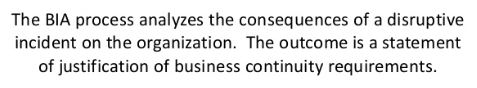
\includegraphics[width=12cm]{BIA.png}
\caption{Definizione di BIA secondo lo Standard ISO 22317 \href{https://www.slideshare.net/TheBCEye/isos-newest-standard-the-bia-iso-22317}{www.slideshare.net/}}
\end{figure}

Nella Business Impact Analysis viene svolta una analisi . In particolare ci si concentrerà sulla prioritizzazione di servizi, processi e attività, sulla base degli effetti o le conseguenze dell'interruzione delle funzioni aziendali IT critiche.
\\In una BIA si dovrebbero anche quantificare i costi associati a un disastro (perdite finanziarie o ripercussioni su relazioni pubbliche, morale, salute e sicurezza o perdita del vantaggio competitivo). Nel presente documento viene accennato il calcolo dei costi, che però dovrebbe essere complementato e completato in presenza di dati più esaurienti.
\\ La BIA deve essere stesa in stretta collaborazione col processo di Risk Management ed è un buon punto di partenza per la valutazione degli obiettivi del tempo di recupero (RTO) e gli obiettivi del punto di ripristino (RPO) e delle risorse e i materiali necessari per la continuità aziendale.
\vspace{0.5cm}
\\ Per la stesura della BIA, ci avvaleremo del corpo centrale del template \textbf{ISO 22317}.
\vspace{0.5cm}
\begin{figure}[H]
\centering
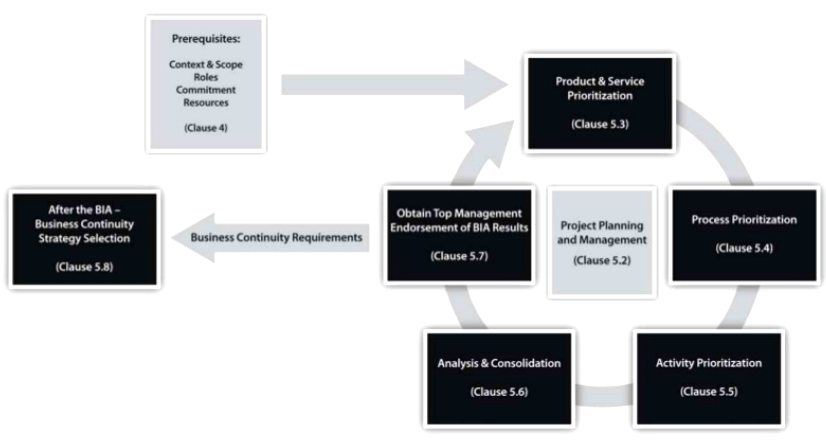
\includegraphics[width=12.5cm]{bia_schema.png}
\caption{Definizione di BIA secondo lo Standard ISO 22317\href{https://www.slideshare.net/TheBCEye/isos-newest-standard-the-bia-iso-22317}{www.slideshare.net/}}
\end{figure}

\newpage
\subsubsection{Product and Service Prioritization}
\begin{figure}[H]
\centering
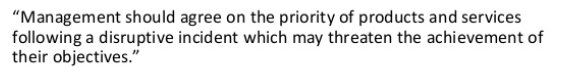
\includegraphics[width=12cm]{BIA_pes.png}
\caption{Definizione di Product and Service Prioritization\href{https://www.slideshare.net/TheBCEye/isos-newest-standard-the-bia-iso-22317}{www.slideshare.net/}}
\end{figure}
In questa sezione viene data una priorità ai servizi oggetto di appalto.\\
La priorità varia in una scala da 1 a 5 dove 1 indica una bassa priorità e 5 indica un'alta priorità.

\renewcommand\arraystretch{1,3}
\begin{longtable}{p{10cm} c}
\toprule
\textbf{Servizio} & \textbf{Priorità} \\
\toprule
Conduzione operativa dei sistemi di elaborazione & 5 \\
Pianificazione e controllo delle elaborazioni & 3 \\
Manutenzione degli ambienti software di sistema & 4 \\
Systems \& LAN Management & 4 \\
\hspace{2cm} tra cui servizio internet generale & 5 \\
\hspace{2cm} tra cui servizio internet dorsale & 4 \\
\hspace{2cm} tra cui servizio internet terminale & 3 \\
Call Center Interno & 3 \\
Gestione della configurazione & 3 \\
Outsourcing delle postazioni di lavoro & 3 \\
Manutenzione del software applicativo & 4 \\
Formazione & 3 \\
Servizio di housing & 5 \\
Servizio di supporto direzionale & 3 \\
Servizio di supporto gestione del personale & 3 \\
\bottomrule
\caption{BIA - Service Prioritization}
\end{longtable}

\newpage
\subsubsection{Process Prioritization}
\begin{figure}[H]
\centering
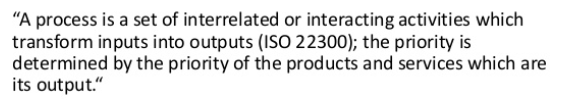
\includegraphics[width=12cm]{BIA_proc.png}
\caption{Definizione di Processo secondo lo Standard ISO \href{https://www.slideshare.net/TheBCEye/isos-newest-standard-the-bia-iso-22317}{www.slideshare.net/}}
\end{figure}
In questa sezione viene data una priorità ai processi dell'Istituto Gaetano Pini, comprendendo sia i processi che l'offrente andrà ad istanziare (come richiesto nel capitolato d'appalto in 5.1.4) sia i processi oggetto di rivisitazione, e descritti nel cap.1 del presente documento.\\
La priorità varia in una scala da 1 a 5 dove 1 indica una bassa priorità e 5 indica un'alta priorità.\\
\renewcommand\arraystretch{1,5}
\begin{longtable}{p{8cm} c}
\toprule
\textbf{Processo} & \textbf{Priorità} \\
\toprule
Asset management & 2 \\
Change management & 2 \\
Problem management & 3 \\
Business continuity & 3 \\
Misurazione dei livelli di servizio & 2 \\
Processo di gestione delle prestazioni ambulatoriali & 3 \\
Processo di gestione delle prestazioni di ricovero & 2 \\
Processo di gestione delle prestazioni di Pronto Soccorso & 5\\
\small{\hspace{1cm} tra cui operazioni coinvolgenti attività di codice giallo e rosso} & 5\\
\small{\hspace{0.5cm} tra cui operazioni coinvolgenti attività di codice bianco e verde e altre operazioni} & 4\\
Processo di gestione risorse economiche & 3 \\
Processo di gestione risorse umane & 2 \\
Processi di gestione direzionale & 2 \\
\bottomrule
\caption{BIA - Process Prioritization}
\end{longtable}

\newpage
\subsubsection{Activity Prioritization}
\begin{figure}[H]
\centering
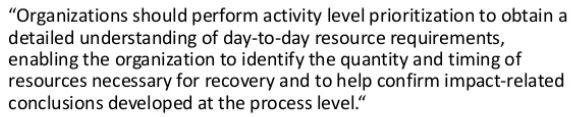
\includegraphics[width=12cm]{BIA_act.png}
\caption{Definizione di Activity Prioritization \href{https://www.slideshare.net/TheBCEye/isos-newest-standard-the-bia-iso-22317}{www.slideshare.net/}}
\end{figure}

In questa sezione viene data una priorità alle attività. Tutto ciò quello che viene definito come \textbf{attività} viene elencato nelle tabelle sottostanti di prioritizzazione delle attività (che partono dalla pagina successiva - per saltare le tabelle vedere in \ref{fineattprio}).\\
La priorità varia in una scala da 1 a 5 dove 1 indica una bassa priorità e 5 indica un'alta priorità.\\

\paragraph{Conduzione operativa dei sistemi di elaborazione}
\textcolor{white}{.} \\
\renewcommand\arraystretch{1,3}
\begin{longtable}{p{12cm} c }
\toprule
\textbf{Attività} & \textbf{Priorità} \\
\toprule
Accensione ed inizializzazione apparecchiature e sistemi, attivazione delle configurazioni (hardware e software)  & 4 \\
Controllo   dei   sistemi   e   del   corretto   funzionamento,   diagnosi   di   primo   livello   dei malfunzionamenti,  attivazione  dei  tecnici  delle  società  preposte  alla  manutenzione  e fornitura del relativo supporto  & 3 \\
Registrazione,   nel   sistema   di   gestione   dei   problemi,   dei   malfunzionamenti   delle 
apparecchiature,della relativa diagnosi, dei conseguenti interventi di ripristino e dello stato degli interventi & 2 \\
Attivazione  e  controllo  elaborazioni  batch  e/o  stampe,  secondo  le  schedulazioni previste,  & 2 \\
Montaggio/smontaggio dei supporti sulle unità di registrazione & 2 \\ 
Attivazione di procedure di salvataggio delle informazioni e delle applicazioni (back up e disaster recovery)  
 & 5 \\
Registrazione delle attività ed elaborazione di statistiche di consuntivo sulla operatività e disponibilità delle apparecchiature e dei sistemi condotti.  & 2 \\
Tenere un giornale delle attività e dei problemi &2 \\
Tenere un riepilogo periodico consuntivo del periodo di osservazione concordato con l’Istituto, che riporti  statistiche  su  operatività  dei  sistemi  e  problemi. & 2 \\
\bottomrule
\caption{BIA - Activity Prioritization - Conduzione operativa dei sistemi di elaborazione}
\end{longtable}

\newpage
\paragraph{Pianificazione e controllo delle elaborazioni}
\textcolor{white}{.} \\
\renewcommand\arraystretch{1,5}
\begin{longtable}{p{11cm} c }
\toprule
\textbf{Attività} & \textbf{Priorità} \\
\toprule
Raccolta delle esigenze relative alle elaborazioni applicative periodiche  & 2 \\
Predisposizione  di  piani  di  lavoro  periodici  (giornalieri,  settimanali,  mensili,  ecc.)  per  le procedure pianificate (es. stampe cedolini, generazione flussi istituzionali, ecc.)  & 3\\
Ricezione e accodamento  richieste  di  attivazione  procedure,  non  pianificate,  e  schedulazione  delle procedure  & 3 \\
Controllo  della  corretta  esecuzione  delle  elaborazioni,  diagnosi  di  primo  livello  dei 
problemi  relativi  alla  esecuzione  di procedure  applicative,  attivazione  dei  tecnici  preposti alla risoluzione e loro supporto  & 3 \\
Registrazione delle attività, dei problemi, degli interventi di correzione anche nel sistema di gestione dei problemi,  & 2 \\
Elaborazione di statistiche di consuntivo  & 2\\
Tenuta di piani di elaborazione, comprensivi delle registrazione delle richieste  & 2\\
Tenuta di  un giornale delle attività effettuate con evidenza di quelle portate a termine correttamente, dei problemi e delle azioni correttive & 2 \\
Tenuta di  un  riepilogo  periodico  consuntivo,  almeno  trimestrale,  che  riporti  statistiche  su  attività  e problemi.  & 2 \\
\bottomrule
\caption{BIA - Activity Prioritization - Pianificazione e controllo delle elaborazioni}
\end{longtable}

\newpage
\paragraph{Manutenzione degli ambienti software di sistema}
\textcolor{white}{.} \\
\renewcommand\arraystretch{1,5}
\begin{longtable}{p{11cm} c }
\toprule
\textbf{Attività} & \textbf{Priorità} \\
\toprule
Aggiornamento   periodico,   programmato   o   estemporaneo,   dei   prodotti   in   base   alle specifiche  di  rilascio  di  nuove  versioni  o  release  o  patch  da  parte  dei  produttori  sia  per correzione  che  per  miglioramento.  L’aggiornamento  avverrà  solo  a  valle  di  verifiche  di compatibilità  delle  nuove  versioni  nell’architettura  complessiva  del  sistema  informatico  e comunque con autorizzazione da parte dell’Istituto.  
 & 2 \\
Manutenzione  programmata  (inclusa  la  dismissione  per  le  soluzioni  obsolete  ed  escluse dall’architettura)  e  soluzione  di  problemi  \textit{estemporanei}  per  componenti  mal  funzionanti, con diagnosi di primo livello, intervento sulla configurazione e attivazione dei tecnici delle società produttrici o di assistenza specifica sul prodotto.    &4 \\
Test  e  collaudo  dell’operatività  dei  sistemi,  dopo  l’aggiornamento  o  l’intervento  di 
manutenzione,   prima   dell’entrata   in   produzione.   A   tal   fine,   come   già   dichiarato 
precedentemente, si dovrà prevedere la presenza di un ambiente  di test nell’architettura 
complessiva del sistema informatico.   &3 \\
Aggiornamento della configurazione in funzione delle modifiche apportate (di versione, di prodotto, ecc.) e registrazione delle attività    & 3 \\
Tenuta di piani periodici di aggiornamento e di manutenzione programmata degli ambienti software di sistema   &2 \\
Tenuta di un  giornale  delle  attività  effettuate  (interventi  programmati,  aggiornamenti  effettuati,  etc.) con evidenza  dei problemi e delle azioni correttive, dei collaudi effettuati prima del rilascio in produzione e delle modifiche effettuate sulla configurazione  & 0 \\
Tenuta di un  riepilogo  periodico  consuntivo,  almeno  trimestrale,  che  riporti  statistiche  su  attività  e problemi. & 2 \\
\bottomrule
\caption{BIA - Activity Prioritization - Manutenzione degli ambienti software di sistema}
\end{longtable}

\newpage
\paragraph{Systems \& LAN Management}
\textcolor{white}{.} \\
\renewcommand\arraystretch{1,5}
\begin{longtable}{p{11cm} c }
\toprule
\textbf{Attività} & \textbf{Priorità} \\
\toprule
Monitoraggio e gestione dei server, delle LAN e dei posti di lavoro (PdL) & 5 \\
Gestione delle password, dei profili utente e degli indirizzi IP per l’accesso dei PdL alle risorse di rete  & 3 \\
Controllo  centralizzato  sulla  gestione  dei  server,  dei  file  system,    dei   profili   utente, gestione remota delle procedure di backup/recovery dei server;  & 5 \\
Monitoraggio  dello  stato  di  funzionamento  delle  singole  componenti  attive  delle LAN, dei firewall e degli apparati di rete  & 3 \\
Rilevazione dei malfunzionamenti degli apparati di rete e la loro gestione, & 5 \\
Rilevazione del traffico, per individuare possibili aree di inefficienza, colli di bottiglia o sintomi di malfunzionamento;   & 3 \\
Software distribution management  & 3 \\
Configuration management & 3\\
Performances analisys & 2 \\
Stampa & 2 \\
\bottomrule
\caption{BIA - Activity Prioritization - Systems \& LAN Management}
\end{longtable}

\newpage
\paragraph{Call Center Interno}
\textcolor{white}{.} \\
\renewcommand\arraystretch{1,3}
\begin{longtable}{p{13cm} c }
\toprule
\textbf{Attività} & \textbf{P.tà} \\
\toprule
Assicurare la comunicazione tempestiva ed efficace con l’utenza & 2 \\
Provvedere all’accoglimento ed alla registrazione delle richieste di assistenza o rigettarle se non di competenza  &2 \\
Risolvere  i  problemi  più  ricorrenti,  di  non  elevata  complessità,  assistenza  agli  utenti  relativamente  alla  fruizione  dei  servizi  del   sistema  informativo,   assistenza  nell'uso appropriato delle funzioni messe a disposizione dal sistema informativo;  & 3 \\
Smistare  al  personale  del  Centro  di  Gestione  e  a  strutture  di  assistenza  specifiche  la risoluzione dei problemi non risolvibili al primo livello,  &2 \\
Controllare i processi di risoluzione attivati e verificarne gli esiti,  & 2\\
Rendicontare all’utente sullo stato dell’intervento e chiudere l’intervento alla risoluzione del problema e/o della richiesta,  & 2  \\
Analizzare  le  statistiche  sugli  interventi,  al  fine  di  identificare  i  fabbisogni  (anche  di formazione) e definire azioni di prevenzione dei problemi.  & 2 \\
rispondere a informazioni sui servizi erogati dal sistema informativo;  & 1 \\
rispondere a assistenza sull’uso dei servizi e delle applicazioni;  & 1 \\
rispondere a eventuali problemi riscontrati;  & 1 \\
effettuare attivazione, (ri)configurazione, sospensione di un servizio;  & 2 \\
fornire risorse informatiche.  &2 \\
sopperire a difetti e/o a malfunzionamenti dei programmi applicativi; & 2 \\
istruire  il  personale  specializzato  per  il  superamento,  la  correzione  o  l'aggiramento  di eventuali errori presenti nei programmi; & 3 \\
fornire  le  nuove  versioni  e  gli  aggiornamenti  del  software  applicativo  e  le  eventuali 
correzioni necessarie per il software di base e d’ambiente; & 3 \\
supportare la installazione di nuove versioni dei programmi o gli aggiornamenti dei software di base e d'ambiente; &2\\
supportare   l'esecuzione   operativa   delle   funzioni   per   quanto   non   espressamente 
documentato nella manualistica d'uso o di gestione, ovvero non opportunamente descritto in sede di addestramento; & 4 \\
dare  assistenza  sistemistica  e  consulenza  riguardo  all’utilizzo  del  software  di  base  ed applicativo e per la risoluzione dei diversi problemi di esercizio connessi al funzionamento delle apparecchiature o all’impiego delle funzionalità applicative. & 3 \\
Tenuta consuntivi &2 \\
\bottomrule
\caption{BIA - Activity Prioritization - Call Center Interno}
\end{longtable}

\newpage
\paragraph{Gestione della configurazione}
\textcolor{white}{.} \\
\renewcommand\arraystretch{1,5}
\begin{longtable}{p{11cm} c }
\toprule
\textbf{Attività} & \textbf{Priorità} \\
\toprule
identificazione  e  gestione  delle  componenti  (configuration  item)  e  dello  stato  delle 
componenti   &3 \\
definizione  delle  procedure  formali  di  modifica  della  configurazione  (responsabilità, 
attività, ecc.)   & 2 \\
controllo  della  configurazione  con  analisi  delle  esigenze  e  delle  richieste  di  modifica, 
registrazione delle modifiche effettuate, archiviazione dei dati relativi,  & 2 \\
valutazione periodica della completezza della configurazione rispetto ai requisiti definiti, & 2 \\
gestione dei rilasci ed installazioni delle versioni delle componenti  & 2 \\
produzione di rapporti periodici ed a richiesta sullo stato della configurazione. & 2 \\
\bottomrule
\caption{BIA - Activity Prioritization - Gestione della configurazione}
\end{longtable}

\newpage
\paragraph{Outsourcing delle postazioni di lavoro}
\textcolor{white}{.} \\
\renewcommand\arraystretch{1,5}
\begin{longtable}{p{11cm} c }
\toprule
\textbf{Attività} & \textbf{Priorità} \\
\toprule
Manutenzione   di   hardware   e   software   di   base   (preventiva,   adattativa,   correttiva), & 4 \\
Installazione di hardware e software, gestione delle modifiche e degli aggiornamenti.  & 3 \\
Gestione  dei  dati  e  delle  configurazioni  degli  utenti  (backup  e  restore,  installazione  e gestione  prodotti  antivirus,  installazione  e  gestione  applicazioni  per  servizi  internet  e 
posta);(l’onere del backup dei documenti e dei dati sulle postazioni, se non legati ad applicazioni centralizzate, resta a carico degli utenti stessi.)  & 3 \\
Gestione delle risorse critiche, con particolare attenzione alle performance ed ai tempi di ripristino;   & 5 \\
Predisposizione rapporti periodici di consuntivazione dei problemi, ed analisi della qualità del  servizio  reso  attraverso  rilevazione  (errori,  chiamate,  tempi  di  attesa,  soddisfazione utente, ecc.)  & 5 \\
\bottomrule
\caption{BIA - Activity Prioritization - Outsourcing delle postazioni di lavoro}
\end{longtable}

\paragraph{Manutenzione del software applicativo}
\textcolor{white}{.} \\
\renewcommand\arraystretch{1,5}
\begin{longtable}{p{11cm} c }
\toprule
\textbf{Attività} & \textbf{Priorità} \\
\toprule
Manutenzione correttiva &5 \\
Manutenzione adeguativa & 3 \\
Manutenzione normativa & 4 \\
Manutenzione migliorativa & 3 \\
Manutenzione evolutiva & 2 \\
Tenuta consuntivi & 2 \\
\bottomrule
\caption{BIA - Activity Prioritization - Manutenzione del software applicativo}
\end{longtable}

\newpage
\paragraph{Formazione}
\textcolor{white}{.} \\
\renewcommand\arraystretch{1,5}
\begin{longtable}{p{11cm} c }
\toprule
\textbf{Attività} & \textbf{Priorità} \\
\toprule
Tenuta lezioni & 3 \\
Tenuta verifiche & 2 \\
Tenuta consuntivi & 2 \\
\bottomrule
\caption{BIA - Activity Prioritization - Formazione}
\end{longtable}

\paragraph{Servizio di supporto direzionale}
\textcolor{white}{.} \\
\renewcommand\arraystretch{1,5}
\begin{longtable}{p{11cm} c }
\toprule
\textbf{Attività} & \textbf{Priorità} \\
\toprule
Analisi dei processi aziendali e dei principali flussi   & 3 \\
Supporto  alla  progettazione  del  sistema  e  dei  processi  per  il  controllo  di  gestione  ed  il budgeting  & 3 \\
Disegno del sistema informativo per  supportare adeguatamente i processi e la raccolta dei 
dati necessari per le funzioni di controllo  & 3 \\
Disegno del sistema di reporting sia in ambito amministrativo che sanitario  & 3 \\
Controllo correttezza dei flussi istituzionali (completezza dei dati raccolti, congruità, ecc.)  & 4 \\
Tenuta consuntivi & 0 \\
\bottomrule
\caption{BIA - Activity Prioritization - Servizio di supporto direzionale}
\end{longtable}

\newpage
\paragraph{Servizio di supporto gestione del personale}
\textcolor{white}{.} \\
\renewcommand\arraystretch{1,5}
\begin{longtable}{p{11cm} c }
\toprule
\textbf{Attività} & \textbf{Priorità} \\
\toprule
Gestione tabellare (aggiornamento dati relativi alle codifiche fondamentali e ai parametri da 
utilizzare nei calcoli e provenienti dalla indicazioni legislative e contrattuali) su indicazione 
del  responsabile  del  servizio  e  con  valutazione  delle  modifiche  indotte  da  variazioni 
legislative)  &4 \\
Cedolini, dichiarazioni, modulistica e in genere elaborati richiesti dalla normativa  & 3 \\
Reportistica standard  & 2 \\
Flussi verso altri sistemi aziendali  & 3 \\
Imbustamento, distribuzione e consegna cedolini con modalità proposta dalle ditte (in sede, 
via postel, etc.)  & 3\\
Gestione badge aziendali (consegna, sostituzione, ritiro, etc.)  & 2\\
Altri servizi di supporto,  proposti dalle ditte, aggiuntivi e ad integrazione di questi già citati.  & 2\\
\bottomrule
\caption{BIA - Activity Prioritization - Servizio di supporto gestione del personale}
\end{longtable}

\paragraph{Altri servizi}
\textcolor{white}{.} \\
\renewcommand\arraystretch{1,5}
\begin{longtable}{p{11cm} c }
\toprule
\textbf{Attività} & \textbf{Priorità} \\
\toprule
Firma digitale & 3 \\
Gestione documentazione & 2 \\
Gestione accesso ai dati & 4 \\
\bottomrule
\caption{BIA - Activity Prioritization - Altri servizi}
\end{longtable}

\newpage
\subsubsection{Analysis and Consolidation} 
\label{fineattprio}
In questa sezione, che deve essere stesa in stretta collaborazione col processo di Risk Management, cercheremo di dare delle linee guida una stima dell'impatto di un evento.\\
Per calcolare la stima degli impatti, useremo come base il modello indicato da \href{http://security.polito.it/~lioy/01jem/risk05_risk_2x.pdf}{security.polito}.
Un \textbf{evento} trae ispirazione, secondo quanto scritto nel capitolato) dai processi dell'Istituto, dai servizi offerti oggetto di appalto, dalle tipologie di prestazione sanitaria effettuate dall'Istituto e dalle fasi sanitarie descritte in ambito CRS-SISS. Segue una breve descrizione di questi punti citati.
\vspace{1cm}
\\
\textbf{Fasi sanitarie in ambito CRS-SISS}
\begin{itemize}
    \item prescrizione 
      \begin{itemize}
          \item identificazione cittadino - IdCitt
          \item prescrizione - Ps
      \end{itemize}
    \item accoglienza
        \begin{itemize}
           \item prenotazione (non presente in fase di pronto soccorso) - Pn
            \item pagamento -  \$
            \item accettazione (identificazione della prescrizione prenotata) - IdPs
         \end{itemize}
    \item erogazione 
        \begin{itemize}
          \item trasferimento (di reparto) - Tr
          \item dismissione - Dism
          \item messa a disposizione del referto - Ref
        \end{itemize}
    \item rendicontazione - Rend
 \end{itemize}
 \vspace{1cm}
 \textbf{Tipologie di prestazione sanitaria effettuate dall'Istituto}
  \begin{itemize}
  \item ortopedia e traumatologia
  \item recupero e riabilitazione funzionale
  \item reumatologia e servizi sanitari di supporto
  \item chirurgia vascolare
  \end{itemize}

\newpage
\paragraph{Moltiplicatore evento}
Per calcolare l'impatto di un evento useremo un apposito \textit{moltiplicatore evento}. La seguente tabella è una tabella ausiliaria utile al calcolo del \textit{moltiplicatore evento}. 
Il moltiplicatore è un primo tentativo di riassumere le attività messe a rischio comprendono persone, proprietà, catena di fornitura, tecnologia informatica, reputazione aziendale e obblighi contrattuali, altrimenti difficilmente valutabili quantitativamente.
\renewcommand\arraystretch{1,2}
\begin{longtable}{p{4cm} c c c c c c c c c}
\toprule
\textbf{Tipologia} & IdCitt & Ps & Pn & \$ & IdPs & Ts & Dism & Ref & Rend \\
\toprule
Ortopedia e traumatologia (base +2) & +1 & 0 & 0 & 0 & 0 & -1 & -1 & -1 & -1 \\
Recupero e riabilitazione funzionale (base 0) & +1 & 0 & 0 & 0 & 0 & -1 & -1 & -1 & -1 \\
Reumatologia e servizi sanitari di supporto (base 0) & +1 & 0 & 0 & 0 & 0 & -1 & -1 & -1 & -1 \\
Chirurgia vascolare (base +1) & +1 & 0 & 0 & 0 & 0 & -1 & -1 & -1 & -1 \\
\bottomrule
\caption{BIA - Bonus fase e tipologia}
\end{longtable}

Per calcolare il moltiplicatore ci si affiderà alla seguente formula: 
\begin{center}
	\line(1,0){350}\\
    \vspace{0,1cm}
	\textit{Molt. evento} = (\textit{Priorità dell'attività}
    		+\textit{Bonus fase e tipologia})
            X \textit{Priorità processo}
	\line(1,0){350}
\end{center}
in cui la \textit{Priorità dell'attività} è data dalle tabelle sottostanti, il \textit{Bonus di fase e tipologia} è data dalla tabella sovrastante, e la \textit{Priorità del processo} è data dalla tabella della \textit{Priorità dei processi}.
\\ Se una attività comporta più conseguenze, in più fasi e/o tipologie e/o in più processi, si effettuerà la sommatoria di ogni conseguenza.
\\ Il \textit{Bonus di fase e tipologia} è da sommare alla \textit{Priorità dell'attività} solo nei casi in cui la classificazione dell'attività per fase e tipologia risulti sensata. I casi esatti saranno  definiti nella fase di progettazione esecutiva della soluzione oggetto di appalto. 

\begin{center}
	\line(1,0){350}
\end{center}
\begin{changemargin}{0.5cm}{0.5cm}
  \textbf{Esempio: accensione sistemi di prenotazione di visite ambulatoriali ortopediche:}\\
  Priorità dell'attività = 4 (accensione)\\
  Bonus di fase e tipologia = 2 (ortopedia e traumatologia Pn)\\
  Priorità del processo coinvolto = 3 (ambulatorio)\\
  \textbf{Moltiplicatore evento} = (4 + 2) x 3 = 18
\end{changemargin}
\begin{center}
	\line(1,0){350}
\end{center}

\paragraph{Stima degli impatti}
Per calcolare la stima degli impatti, useremo come base il modello indicato da \href{http://security.polito.it/~lioy/01jem/risk05_risk_2x.pdf}{security.polito}.\\
L'impatto di un evento (es: mancata accensione dei sistemi di prenotazione di visite ambulatoriali ortopediche) viene calcolato come:
\\
\begin{center}
	\line(1,0){350}
    \vspace{0,1cm}
\textit{impatto(evento)} = \textit{valore asset} X \textit{danno\%} X \textit{moltiplicatore evento}
	\line(1,0){350}
\end{center}
in cui:
\begin{itemize}
\item \textit{valore asset} è il valore dell'asset coinvolto direttamente nell'evento. Questo valore è da determinare in collaborazione con i processi di configuration management.
\item \textit{danno\%} è il valore in percentuale del danneggiamento;
\item \textit{moltiplicatore evento} è il numero calcolato al punto precedente.
\end{itemize}

\begin{center}
	\line(1,0){350}
\end{center}
\begin{changemargin}{0.5cm}{0.5cm}
  \textbf{Esempi:}
  \vspace{0.2cm}\\
  \textbf{Mancata accensione dei sistemi di prenotazione di visite ambulatoriali ortopediche:}\\
  Server Aurora = (es:500 000 euro) \\
  Danno\% = 0,01\% \\
  Moltiplicatore\% = 15 \\
  \textbf{Impatto} = (500 000 * 0,01\%) x 18 = 900 euro
  \vspace{0.2cm} \\
  \textbf{Mancata rilevazione dei malfunzionamenti al server di Aurora con conseguenze in pronto soccorso d'urgenza in fase di identificazione cittadino nell'area di traumatologia:}\\
  Server Aurora = (es:500 000 euro) \\
  Danno\% = 0,1\% \\
  Moltiplicatore\% = (5+3) * 5 = 40 \\
  \textbf{Impatto} = (500 000 * 0,1\%) x 40 = 20 000 euro
\end{changemargin}
\begin{center}
	\line(1,0){350}
\end{center}
Se un evento colpisce più asset, si effettuerà la sommatoria per asset. Questa analisi tuttavia non è esaustiva per molti aspetti. In fase di progettazione esecutiva dovranno essere considerati inoltre i seguenti aspetti:
\begin{itemize}
\item fattore tempo: la durata di tempo in cui si protrae il problema influsce nella stima degli impatti;
\item modalità di determinazione del danno in percentuale in modo esatto: deve essere stabilito con chiarezza chi ha il diritto/dovere di effettuare stime per questo dato;
\item modalità di determinazione dell'asset: in base alla definizione di asset, l'importo di questo dato può variare di molto (es: è asset l'intero SAP o i sono asset i suoi moduli?)
\end{itemize}
\vspace{1cm}
A quel punto, si potrà estrarre un elenco di eventi con quantificazione dell'impatto. Ai fini del progetto didattico ci limitiamo ad affermare che possiamo osservare che ci sono processi, attività e servizi che sono cruciali per il business dell'Istituto e che dovranno essere maggiormente soggette a protezione e controlli nella stesura della soluzione di continuità.

\newpage
\subsection{Criticità sistemi e applicativi}
\label{critsisapp}
Sulla base della Business Impact Analysis è possibile stendere la tabella delle criticità dei sistemi e applicativi. Per ognuno di questi si dovrebbe avere la lista dei CI correlati (nella documentazione stesa grazie alla collaborazione dei processi di Risk Management e del SACM), per poi assegnare una priorità ad ogni CI. Ai fini del progetto didattico si ritiene opportuno fermarsi alla tabella della criticità di sistemi e applicativi.

        \renewcommand\arraystretch{1.5}
        \begin{longtable}{c l c c c}
        \toprule
        \textbf{Ambito} & \textbf{Tecnologie} & \textbf{Criticità} \\
        \toprule
            \small{Urgenza, Ambulatorio e Degenza} & Aurora Web, ICAN &  5 \\
            %5 & Immagini & \small{RIS/PACS, AGFA/FUJI} & Dir. Img & 50 \\
             Emoderivati & SAP & 4 \\
             Analisi & PowerLab & 5 \\
             \small{Fatturaz., Archivio clinico, Referti} & SAP &  3 \\
            %4 & Punti gialli & NA & Dir. PtiGialli & ND\\
             SISS & ICAN & 3 \\
             Amministrazione & SAP & 2 \\
             \small{Ricoveri, Sale operatorie, Protesi} & SAP &  4 \\
             Gestione mail & SAP & 2 \\
             Gestione pazienti esterni & SAP  & 3 \\
             Gestione stampa & SAP & 2 \\
            \bottomrule
            \caption{Sistemi e applicativi della soluzione.}
        \end{longtable}


\newpage
\subsection{Valutazione dei rischi}
\label{rischi}
Lo scopo di questa sezione è quello di riportare alcuni dati che sarebbero in possesso del processo di Risk Management (e del SACM) che si occupa di identificare potenziali pericoli e valutare le sue le  vulnerabilità dell'Istituto rispetto ad esse.
\vspace{0.5cm} \\
Nella documentazione stesa grazie alla collaborazione dei processi di Risk Management e del SACM dovrebbero figurare, tra le varie, i CI che potrebbero essere messi in rischio. Ci dovrebbero essere quindi gli elenchi di hardware, software e dei dati critici e diagrammi che rappresentano le dipendenze tra essi. 
Il processo di Risk Management stabilirà come valutare questi dati (es. CRAMM) in suo possesso, in modo da rendere disponibile una stima più precisa dei livelli di rischio. Durante la fase di valutazione del rischio, i risultati della BIA possono essere esaminati rispetto a vari scenari di pericolo e le potenziali interruzioni possono essere prioritarie in base alla probabilità del rischio e alla probabilità di impatto negativo sulle operazioni commerciali.
\vspace{0.5cm} \\
Ai fini del progetto didattico si ritiene opportuno fermarsi alla tabella sottostante che mostra l'elenco dei rischi identificati con associati il livello di minaccia e di vunerabilità. Per ognuna delle seguenti voci sono state consultate fonti autorevoli (es. Terremoto: \href{https://www.thelocal.it/20161028/which-areas-of-italy-have-the-highest-risk-of-earthquakes}{thelocal.it}
\vspace{0.5cm} \\
Queste analisi verranno usate per giustificare gli investimenti in prevenzione e mitigazione, nonché la strategia di continuità che verrà identificata nelle pagine seguenti.
\newpage
\paragraph{Rischi}
\textcolor{white}{.} \\
\renewcommand\arraystretch{1,5}
\begin{longtable}{p{7cm} c c c }
\toprule
\textbf{Evento} & \textbf{Minaccia} & \textbf{Vulnerabilità}\\
\toprule
Terremoto & 1 & 2 \\
Allagamento & 3 & 3 \\
Uragano & 1 & 4 \\
Incendio & 4 & 1 \\
Interruzione dell'erogazione del servizio da parte del fornitore di SAP & 4 & 2 \\
"" "" di Aurora Web & 5 & 2 \\
"" "" di PowerLab & 4 & 2 \\
"" "" del SISS & 6 & 4 \\
Indisponibilità generica di corrente elettrica & 8 & 5 \\
Interruzione cablaggio dorsale & 3 & 4 \\
Interruzione cablaggio terminale & 2 & 3 \\
Attacco informatico (dati rubati) a SAP o Aurora o cache ICAN-SISS& 3 & 2 \\
Attacco informatico (dati rubati) a PowerLab& 2 & 2 \\
Attacco informatico (dati editati o cancellati) a SAP o Aurora o ICAN-SISS& 3 & 2 \\
Attacco informatico (dati editati o cancellati) a PowerLab& 2 & 2 \\
Attacco informatico (ddos o simili) a sistemi SAP o Aurora o ICAN-SISS& 3 & 2 \\
"" "" PowerLab & 2 & 2 \\
"" "" di ridondanza& 2 & 2 \\
Indisponibilità di persone chiave & 4 & 3 \\
\bottomrule
\caption{BIA - Valutazione dei rischi}
\end{longtable}


\newpage
\subsection{Identificazione RTO e RPO}
\label{rtorpo}
L'RPO (RecoveryPoint Objective) è la perdita dati tollerata (in tempo) mentre l'RTO (RecoveryTime Objective) è il tempo di ripristino servizio. La seguente figura mostra graficamente e dà una definizione formale di questi due termini. \\ Si riportano gli RTO e gli RPO per ogni applicativo/sistema risultanti dall'analisi effettuata tramite BIA, prioritizzazione sistemi e applicativi e prioritizzazione rischi.

\begin{figure}[H]
\centering
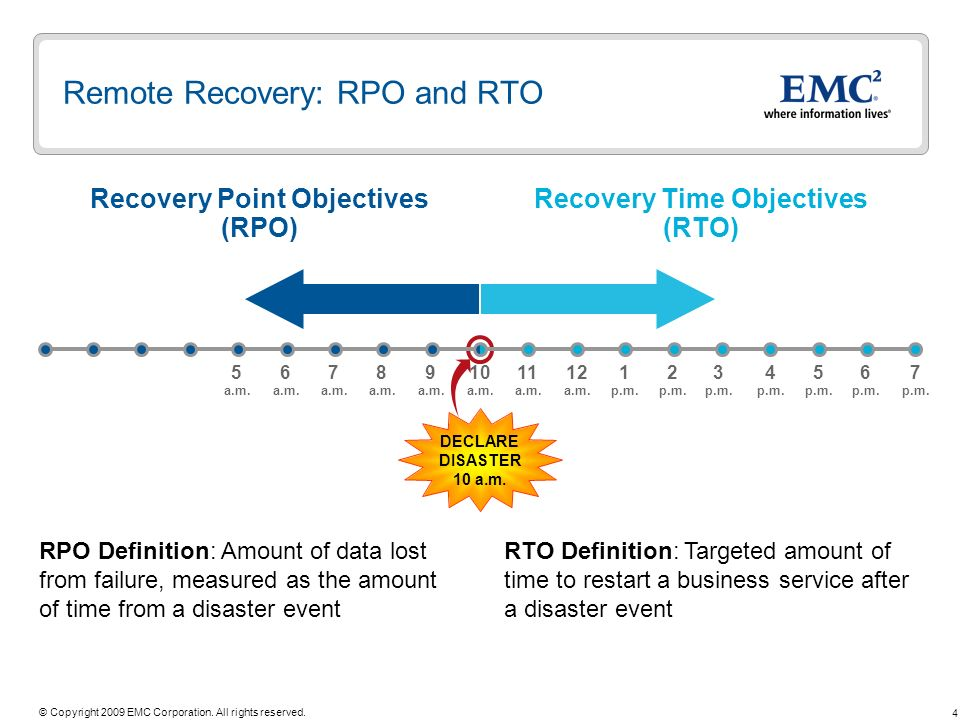
\includegraphics[width=14cm]{RPORTOdef.jpg}
\caption{Tempo e costo di recovery \href{https://slideplayer.com/slide/231966/}{slideplayer}}
\end{figure}

\renewcommand\arraystretch{1,5}
\begin{longtable}{p{5cm} p{2.5cm} c c }
\toprule
\textbf{Applicativo o sistema} & \textbf{Tecnologia} & \textbf{RTO} & \textbf{RPO} \\
\toprule
	Urgenza & Aurora Web & 15 minuti & 4 ore \\
    Ambulatorio & Aurora Web &4 ore & 4 ore \\
	Degenza & Aurora Web & 3 giorni & 8 ore \\
	Emoderivati & SAP & 8 ore & 8 ore \\
    Analisi & PowerLab & 1 ora & 8 ore \\
    Fatturazione & SAP & 1 settimana & 8 ore\\
    Archivio clinico & SAP & 1 settimana & 3 giorni\\
    Referti & SAP & 1 settimana & 3 giorni\\
    SISS & ICAN & 8 ore & 8 ore\\
    Direzione & SAP & 1 settimana & 8 ore\\
    Risorse umane & SAP & 1 settimana & 8 ore\\
    Ricoveri & SAP & 1 settimana & 8 ore\\
    Sale operatorie & SAP & 3 giorni & 4 ore\\
    Protesi & SAP & 3 giorni & 8 ore\\
    Mail & SAP & 8 ore & 4 ore\\
    Pazienti esterni & SAP & 8 ore & 8 ore\\
    Stampa & SAP & 1 settimana &  1 settimana\\
\bottomrule
\caption{RTO e RPO }
\end{longtable}







































%*******************************************************
\newpage
\section{Strategy Definition}
Sulla base della BIA, del Risk Assessment e degli RTO e RPO concordati, viene definita la strategia di continuità IT, con l'obbiettivo di di raggiungere l'equilibrio ottimale tra la minimizzazione del rischio e la razionalizzazione costo di gestione della continuità.\\

\subsection{Le opzioni}
Sono possibili 7 possibilità, dette Tier. La seguente tabella illustra i principali Tier, mostrando i relativi tempi di RTO e RPO. Il grafico mostra le riassume, mostrando la relazione tra costi e tempo di recovery per ogni tier.

\renewcommand\arraystretch{1,5}
\begin{longtable}{p{3,5cm} p{6,5cm} p{1,5cm} p{1,5cm} }
\toprule
\textbf{Tier} & Descrizione & RTO & RPO \\
\toprule
Tier-2: Data backup with a hot site &
regular backups on tape + hot site &
> 3 g. & 1-2 g. \\
Tier-3: \hspace{2cm} Electronic vaulting &
regular backups on tape + hot site + some data is electronically vaulted &
1g-3g. & <= 1g. \\
Tier-4: \hspace{2cm} Point-in-time copies &
more disk based solution (greater frequency) &
4h - 1g. & <= 4h \\
Tier-5: Transaction integrity
& synchronous data copy, atomic transaction &
1h-4h & <= 5min \\
Tier-6: \hspace{2cm} Siti paritetici &
mirroring of data to a remote server - solution independent from the SW used &
<= 1h & real time \\
\bottomrule
\caption{I 7 tier}
\end{longtable}

\begin{figure}[H]
\centering
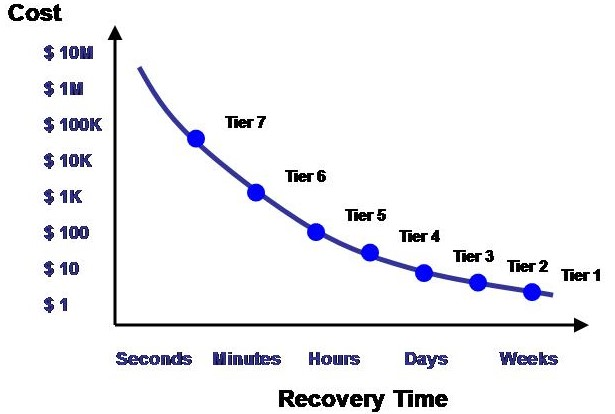
\includegraphics[width=12cm]{time345.jpg}
\caption{Tempo e costo di recovery \href{https://carlgusler.wordpress.com/2008/05/07/seven-levels-of-disaster-recovery-protection/}{carlgusler.wordpress.com}}
\end{figure}

\subsection{I tier richiesti}
In base alle tabelle precedenti possiamo ricavare i Tier richiesti per ogni applicativo/sistema.
\renewcommand\arraystretch{1,5}
\begin{longtable}{p{4cm} c c c c }
\toprule
\textbf{Applicativo o sistema} & \textbf{Tier} & \textbf{Tecnologia} & \textbf{RTO} & \textbf{RPO} \\
\toprule
	Urgenza 		& \textbf{5} & Aurora Web & 30 minuti & 60 minuti \\
    Ambulatorio		& 4 & Aurora Web &4 ore & 4 ore  \\
	Degenza 		& 3 & Aurora Web & 3 giorni & 8 ore \\
	Emoderivati 	& 4 & SAP & 8 ore & 8 ore \\
    Analisi 		& \textbf{5} & PowerLab & 1 ora & 4 ore \\
    Fatturazione 	& 3 & SAP & 1 settimana & 3 giorni \\
    Archivio clinico & 3 & SAP & 1 settimana & 3 giorni \\
    Referti 		& 3 & SAP & 1 settimana & 3 giorni \\
    SISS 			& 4 & ICAN & 8 ore & 4 ore \\
    Direzione 		& 3 & SAP & 1 settimana & 8 ore \\
    Risorse umane 	& 3 & SAP & 1 settimana & 8 ore \\
    Ricoveri 		& 3 & SAP & 1 settimana & 8 ore \\
    Sale operatorie & 4 & SAP & 3 giorni & 4 ore \\
    Protesi 		& 4 & SAP & 3 giorni & 4 ore \\
    Mail 			& 3 & SAP & 8 ore & 8 ore \\
    Pazienti esterni & 4 & SAP & 8 ore & 4 ore \\
    Stampa 			& 3 & SAP & 1 settimana &  1 settimana \\
\bottomrule
\caption{RTO e RPO }
\end{longtable}

\subsection{La scelta}
Per una scelta pienamente completa e consapevole, si dovrebbero avere dati riguardo i costi di avviamento e sostenimento delle varie soluzioni. Al fine del progetto didattico, ipotizziamo che, date le sostanziali risorse economiche e fisiche richieste per implementare il tier 4, e visti costi e benefici per l'implementazione dell'aggiuntivo tier 3, si ritiene opportuno utilizzare le infrastrutture e tecnologie usate per i servizi ospedalieri coperti da tier 4 anche per i servizi ospedalieri che in realtà richiederebbero solo un tier 3. In questo modo i costi di attivazione e mantenimento del tier 4 viene ripartito tra più servizi ospedalieri.
Riassumendo la soluzione è la seguente:
\renewcommand\arraystretch{1,5}
\begin{longtable}{p{4cm} c c c }
\toprule
\textbf{Tecnologia} & \textbf{Tier} & \textbf{RTO} & \textbf{RPO} \\
\toprule
	Aurora Web 	& 5 & 30 minuti & 60 minuti \\
    PowerLab 	& 5 & 1 ora 	& 4 ore \\
    SISS 		& 4 & 8 ore 	& 4 ore \\
	SAP 		& 4 & 8 ore 	& 4 ore\\
\bottomrule
\caption{RTO e RPO - Tecnologie e tier}
\end{longtable}

\subsection{Tempi e modalità di realizzazione della soluzione}
\label{ScadenzaContinuità}
L'implementazione delle soluzioni in modo completo e funzionanete, verrà realizzata nell'arco di 34 mesi per il Tier 4, mentre di 28 mesi per il Tier 5. Tuttavia tutta una serie di sistemi secondari potranno essere pronti prima di tale data, in modo concorde all'avanzamento dei lavori nel progetto, con possibilmente soluzioni di carattere temporaneo. La soluzione di continuità riguarda in ogni caso servizi e sistemi da noi erogati, iscritti in progetto.
\renewcommand\arraystretch{1,3}
\begin{longtable}{p{3cm} p{6cm}}
\toprule
\textbf{Tier} & \textbf{Tempo di realizzazione} \\
\toprule
    Tier 4 & 30 mesi \\
    Tier 5 & 24 mesi \\
\bottomrule
\caption{Tempi di realizzazione}
\end{longtable}

Segue il diagramma di Gantt con la schedulazione dei task ad alto livello da mettere in atto per la realizzazione della soluzione. Il diagramma rappresenta i task ad alto livello.

\begin{figure}[H]
\centering
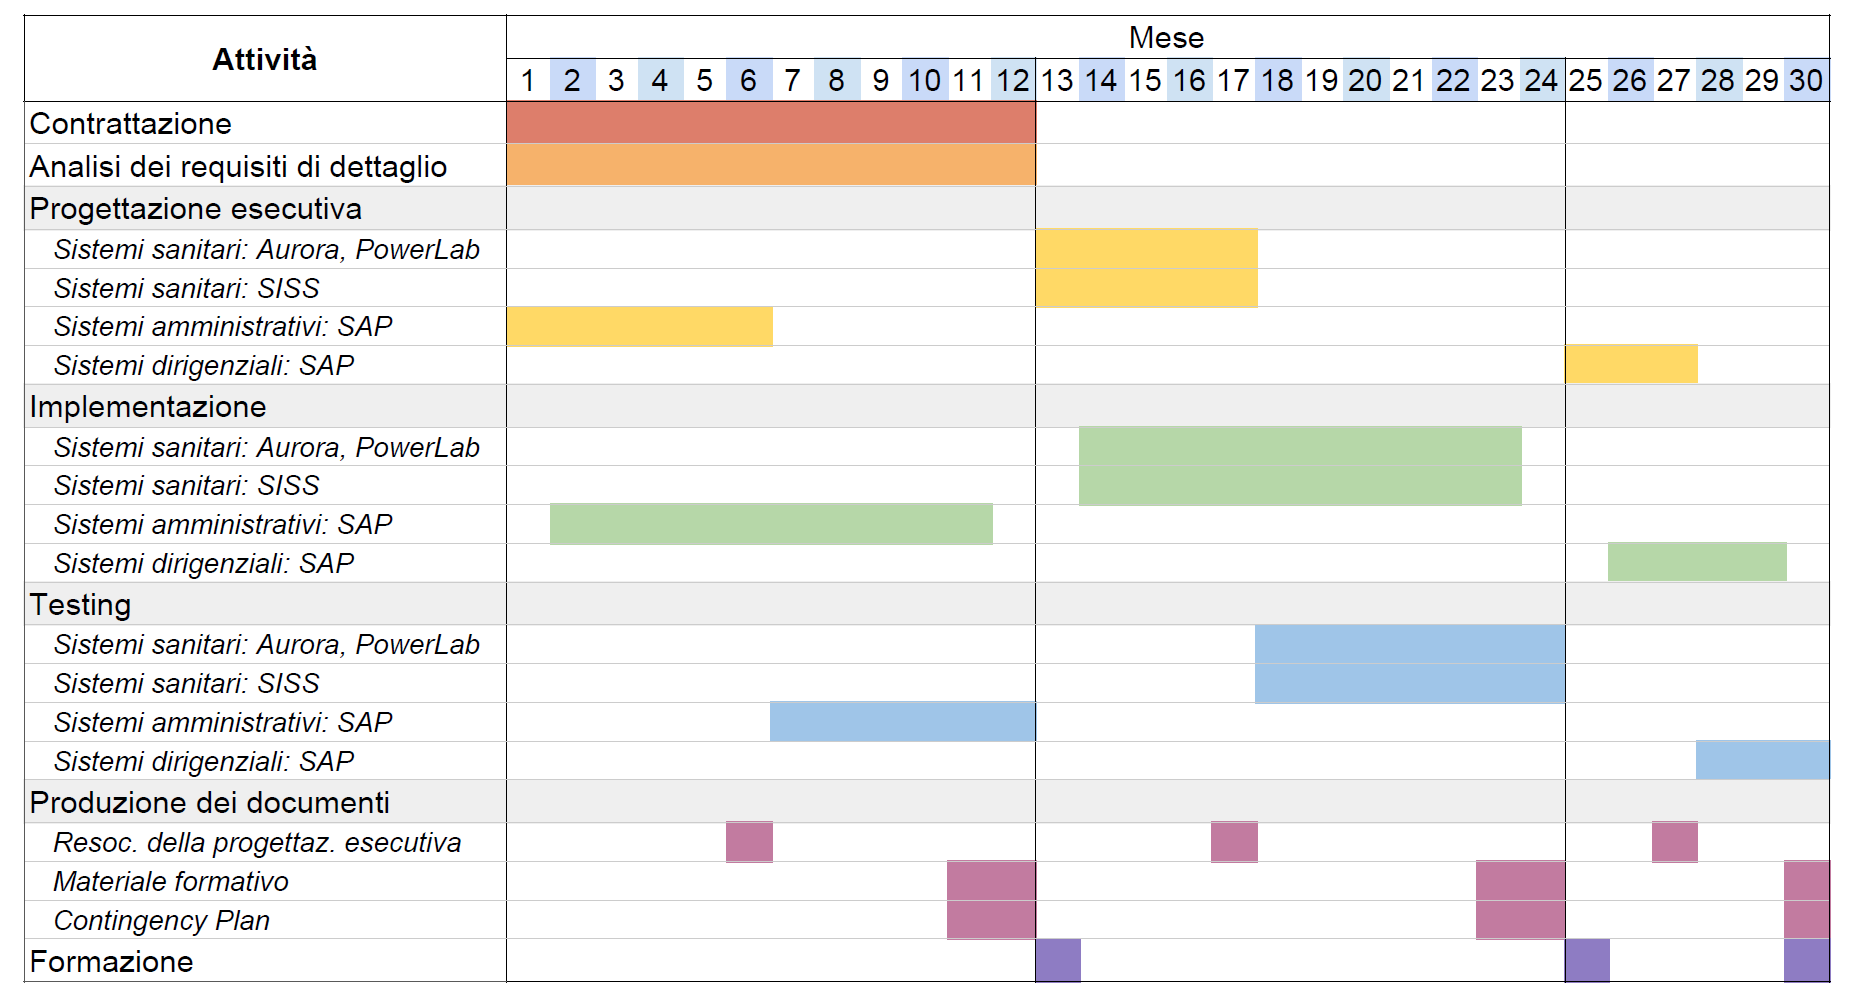
\includegraphics[width=14cm]{gantt-cont.PNG}
\caption{Diagramma di Gantt per la Continuità}
\end{figure}

\subsection{Trasferimento dati tra i siti}
\subsubsection{Caricamento iniziale dei dati}
In fase di caricamento iniziale dei dati nel sito secondario e in fase di rientro presso il sito primario, potranno essere usate anche soluzioni off-line. Una stima sommaria dei dati variati a livello giornaliero indica un ordine di grandezza di decine di TB. Per una stima dettagliata si dovrebbe avere il parere del Capacity Management.
\\Il trasferimento dati può essere relativo a dati sensibili. Vedere la sezione relativa in \ref{cap:rolloutplan}.
\subsubsection{Trasmissione periodica dei dati variati} In considerazione:
\begin{itemize}
\item dei volumi di dati ipotizzati;
\item della distribuzione oraria della finestra di produzione degli aggiornamenti dei dati operati dai servizi oggetto di 
soluzione, concentrata sostanzialmente nella fascia oraria 9.00 – 18.00 dei giorni feriali;
\item del valore di RPO previsto per i servizi oggetto di
 soluzione, variabile tra 60 minuti, 4 ore, 8 ore (e oltre)
\end{itemize}
E' prevista la trasmissione on-line dei dati variati. Parametri di disponibilità, velocità di trasferimento e sicurezza (sia della linea, sia delle caratteristiche dipendenti dalla quantità di dati da trasportare), verranno determinati con maggiore certezza e grado di dettaglio in sede di progettazione esecutiva in collaborazione col Capacity Management. Una stima sommaria dei dati variati a livello giornaliero indica un volume orientativo di alcune centinaia di GB. Al momento si ipotizza una banda di 100Mbps.\\ 	\\
La periodicità degli back-up sarà \textbf{almeno giornaliera} per tutti i servizi, con meccanismi automatici. 
Vedere la sezione di implementazione in \ref{implementation} per maggiori dettagli.
% \begin{itemize}
% \item Per i sistemi \textbf{SISS}, \textbf{PowerLab} e \textbf{ICAN} è previsto almeno un ulteriore salvataggio, da stabilire in sede di progettazione esecutiva. Ad ora si ipotizza un salvataggio aggiuntivo indicativamente a metà giornata lavorativa, per venire incontro ai requisiti di RPO esposti in precedenza.
% \item Per \textbf{Aurora Web} verrà ipotizzata una soluzione ad-hoc viste le prioritizzazioni dei processi e servizi associati a tale tecnologia, che garantisca il soddisfacimento dei requisiti richiesti.
% \end{itemize}
% La banda garantita sarà condivisa tra i servizi distribuendo gli eventi di aggiornamento in modo da evitare conflitto nell’accesso alla risorsa. 
% \\Il trasferimento dati può essere relativo a dati sensibili. Vedere la sezione relativa in \ref{cap:rolloutplan}.

\subsection{Risorse elaborative nel sito primario}
Il tipo di risorse elaborative nel sito primario è misto. 
Sono presenti sia infrastrutture di tipo virtuale che fisico. Il processo di SACM si occuperà di elencare in modo dettagliato i CI presenti nel sito primario.

\subsection{Risorse elaborative previste nel sito secondario}
In coerenza con il Tier 4 individuato, la soluzione prevede che le risorse elaborative nel sito secondario siano sempre disponibili e coerenti con quelle del sito primario, permettendo la ripartenza delle funzionalità in tempi rapidi.\\ 
Le risorse elaborative nel sito secondario saranno basate su una 
infrastruttura hardware in grado di operare su un 
numero di server virtuali sufficienti ad assolvere alle
esigenze di elaborazione del sito primario, completate
da un pool di macchine fisiche volte a raccogliere le
esigenze elaborative non coperte da ambienti virtuali.Si prevede 
la virtualizzazione dei desktop in modo da offrire posti 
di lavoro fruibili localmente o via VPN.
Un dimensionamento preciso verrà effettuato in fase di progettazione esecutiva.


\subsection{Storage, connettività e numero di Postazioni di Lavoro (PdL)}
Gli storage dei siti primari a livello di server hanno dimensioni nell'ordine di decine di TB. Presso il sito secondario si prevedono risoprse tra il 75 e il 100\% dei TB presenti nel sito primario.
\\ E' garantita la copertura di rete nel sito secondario. La banda esatta verrà determinata in sede di progettazione esecutiva.
\\ Nel sito secondario si prevede un numero di PdL utilizzabili 
prevalentemente per attività di back office in numero ridotto 
rispetto a quanto presente nella sede di normale operatività (tra 400 e 500). Il numero esatto verrà stabilito in sede di progettazione esecutiva, ma al momento si stima un numero di PdL compreso tra 30 e 80. Le modalità e i tempi di approvvigionamento e operatività delle risorse in linea di massima sono deducibili dal Gantt soprariportato.
L'Offerente si preoccuperà di descrivere la rete interna (cablaggio, router, switch, firewall, ecc.).
%todo Descrizione della rete interna (cablaggio, router, switch, firewall, ecc.)

\subsection{Localizzazione della struttura di continuità IT}
I  principali  fattori  che  sono stati valutati  nella  scelta  della  localizzazione  del sito secondario  sono  i seguenti:
\begin{itemize}
\item fattori geo-climatici;
\item disponibilità di infrastrutture per le telecomunicazioni;
\item impatto del fattore distanza/vicinanza;
\end{itemize}
E' stata scelta la struttura X in via Y n. Z a Cremona come struttura di continuità IT.
La struttura sarà adatta alle \hyperref{https://www.agid.gov.it}{linee guida Agid} per quanto riguarda:
\begin{itemize}
\item pavimenti e solai;
\item sistemi di illuminazione;
\item cablaggi e telecomunicazioni;
\item armadi e rack;
\item sistemi di raffreddamento e climatizzazione
\item alimentazione e continuità elettrica;
\item antincendio e anti-allagamento.
\end{itemize}

\subsection{Accessi fisici al sito secondario}
Al sito si accederà sia partendo dall'Istituto che partendo dalla sede dell'Offerente tramite automobile e autostrada. Nel retro dello stabile è disponibile un parcheggio gratuito, e affianco un parcheggio a pagamento.
\\
Per accedere fisicamente al sito secondario servono le autorizzazioni scritte (cartacee o elettroniche) dell'IT SC Manager (o del Vice SC Manager) o di un membro dell'IT SC Team.

\subsection{Personale all'interno della struttura secondaria in modalità standard}
Sarà presente fisicamente un operatore designato dall'Offerente a tenere controllato il sito secondario in orario 9-13 e 14-18. L'operatore non necessita di permessi per l'accesso fisico al sito secondario. La lista di operazioni, azioni e responsabilità a suo carico sono da definire con maggiore dettaglio in sede di progettazione esecutiva. Un esempio di operazione potrebbe essere la verfica dell'allineamento dei dati tra le due strutture a campione manualmente almeno una volta al giorno.

\subsection{Work-around manuali}
\label{workaround}
La soluzione individuata come Tier-4 potrebbe portare alla perdita dei dati prodotti nelle ore precendenti allo stato di emergenza, e potrebbe portare alla indisponibilità dei servizi per alcune ore dopo la dichiarazione dello stato di emergenza. Questi dati sono da considerare \textbf{persi} ai fini della soluzione di continuità aziendale. \\ Tuttavia per tentare di arginare i disagi dovuti a questo, si individuerà una serie di work-around manuali di modo che i processi ospedalieri possano continuare anche in situazione di emergenza, previa collaborazione del personale. Alcuni esempi possono essere individuati nella seguente lista, altri dettagli potranno essere aggiunti in fase di progettazione esecutiva.
\begin{itemize}
\item l'offerente si occuperà dell'hosting di una cartella condivisa tra tutti i dipendenti dell'Istituto;
\item all'interno della cartella ci saranno fogli di lavoro pre-impostati da definire con maggiore dettaglio in fase di progettazione esecutiva;
\item ogni dipendente dell'Istituto deve essere dotato di uno smartphone con connessione 3g e con accesso configurato alla cartella condivisa;
\item dal momento di dichiarazione dello stato di emergenza ogni dipendente è invitato a riportare ogni azione e operazione eseguita all'interno dei sistemi informatici nelle ultime quattro ore antecedenti alla dichiarazione;
\item per la gestione dei processi ospedalieri si farà riferimento, oltre che ai dati disponibili nei sistemi ordinari, anche alle informazioni trascritte nei fogli di lavoro suddetti.
\end{itemize}

\subsection{Doppiaggio linea telefonica, elettrica, internet}
Per ovviare ai disagi più comuni di interruzione di fornitura di corrente elettrica, linea telefonica o internet, è previsto di stilare contratti con fornitori terzi (diversi da quelli standard) appositamente per garantire un livello di continuità, seppur ridotto, sufficiente alla conduzione dei processi ospedalieri più importanti.
Si valuteranno attentamente alternative sia di prezzo ma soprattutto di modalità: collegamenti radio (es: Eolo), via terra o con altri mezzi). Si deve grantire un sistema di generazione e distribuzione dell’energia elettrica ridondato. La logica  di  ridondanza  si  deve  avvalere  di  apparecchiature  quali  UPS,  batterie  tampone,  gruppi elettrogeni  a  garanzia  della  continuità  di  erogazione  a  fronte  di  guasti  della  rete  di  distribuzione primaria. 

\subsection{Variazioni nei processi e servizi in fase di emergenza}
\begin{itemize}
\item \textbf{Formazione:} le attività del processo  di formazione vengono sospese fino al rientro completo dalla fase di emergenza;
\item \textbf{Documentazione:} le attività di documentazione e reporting richieste potranno subire dei ritardi; ad ogni modo ci si aspetta che al rientro vengano completati i documenti e i report richiesti entro un mese. Al rientro dalla situazione di emergenza, come previsto in \textit{Operational Management} in \pageref{rientro} si deve stilare un report sull'emergenza avvenuta.
\item \textbf{Service Level Management:} gli SLA in situazione di emergenza non subiranno variazioni;
\item \textbf{Change Management:} potranno essere aperte emergency-RFC in situazione di emergenza. Sarà poi competenza del processo di Change Management stabilire come gestire le emergency-RFC in emergenza in modo da garantire il bilanciamento tra tempi rapidi di risposta e sicurezza e correttezza nel cambiamento;
\item \textbf{Problem Management e Call Center Interno:} Il call center interno potrebbe essere ridotto in quanto a numeri del personale (perlomeno in fase di reazione all'emergenza). E' compito della funzione del Service Desk valutare se riorganizzare le procedure in situazione di emergenza, in modo da garantire il bilanciamento tra velocità e qualità di risposta;
%\item \textbf{Configuration Management:} 
\item \textbf{Processi ospedalieri: } per la gestione dei processi ospedalieri si farà riferimento, oltre che ai dati disponibili nei sistemi ordinari, anche alle informazioni trascritte nei fogli di lavoro suddetti in \ref{workaround}.
\end{itemize}


















































%*******************************************************
\newpage
\section{Implementation}
\label{implementation}

Sulla base della strategia concordata, viene pianificata l'implementazione, coinvolgendo i team IT nella parte di maggior dettaglio.
In questa fase sono previste:
\begin{itemize}
\item ulteriori analisi di dettaglio;
\item progettazione ad alto livello della soluzione di continuità;
\item progettazione esecutiva con sviluppo dei piani implementativi di dettaglio;
\item implementazioni di eventuali misure temporanee;
\item implementazione delle contromisure per la riduzione del rischio e dell'impatto. In particolare il Risk Management metterà in atto tutta una serie di contromisure preventive per i rischi identificati, quali incendi, allagamenti (es: posizionamento porte tagliafuoco, armadi appositi, ventole, raffreddamento).
\item testing.
\end{itemize}

Segue la progettazione ad alto livello della soluzione di continuità divisa per macro-tecnologia.

\newpage
\subsection{Soluzione di Continuità per Aurora Web e PowerLab}
\subsubsection{Interrelazioni con entità esterne all’Amministrazione}
I contratti in essere che vengono coinvolti sono:
\renewcommand \arraystretch{1,5}
\begin{longtable}{c c c}
\toprule
\textbf{Contratto in Essere} & \textbf{Fornitore} & \textbf{Produttore} \\
\toprule
	Contratto unico per fornitura servizi IT & Offerente & Offerente \\
\bottomrule
\caption{Contratti Aurora Web e PowerLab}
\end{longtable}
Non si rilevano necessità di effettuare variazioni contrattuali ai contratti sopracitati.

\subsubsection{Soluzione}
Per Aurora Web e PowerLab è prevista l'adozione del Tier 5.
\begin{figure}[H]
\centering
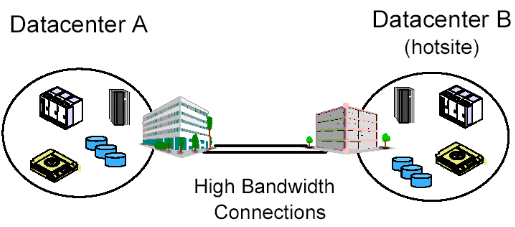
\includegraphics[width=8cm]{tier5.png}
\caption{Tier 5 \href{https://www.abzsol.com/cms/images/stories/pdf/business_continuity.pdf}{www.abzsol.com}}
\end{figure}
Sono previsti:
\begin{itemize}
\item backup off-site radicale ogni sei mesi su nastro da conservare presso l'\textit{Offerente};
%\item backup off-site incrementale una volta al giorno su disco da conservare presso l'hot site;
\item software di gestione Disaster Recovery (da stabilire in progettazione esecutiva es: Tivoli IBM);
%\item piano di Disaster Recovery di dettaglio da stilare in fase di progettazione esecutiva; 
\item hot-site con installazione del server di Aurora Web e PowerLab (con relative librerie e documentazione).
\end{itemize}
I due siti (primario e secondario) sono sincronizzati utilizzando una high-band connession. Gli aggiornamenti ai dati relativi ad Aurora saranno applicati in modo automatizzato sia al server locale, sia al server remoto, usando \textit{single-commit scope} che garantisce che i dati sul sito remoto e sul sito primario vengono aggiornati o retrocessi come un'unica unità di lavoro (UOW). I dati critici e le applicazioni sono quindi presenti su entrambi i siti e vengono persi solo i dati in transizione durante un disastro.\\
Altri dati necessari per eseguire l'applicazione (librerie, documentazione, copie delle licenze software) vengono inviati anche al sito secondario attraverso il software di gestione del DR al momento della creazione della soluzione. Il software permetterà anche il monitoraggio e il controllo della situazione in ogni momento sia antecedente all'emergenza, sia in fase di emergenza, che di rientro.

\subsubsection{Fase di reazione all’emergenza}
Istruzioni operative del start-up di dettaglio verranno fornite in sede di progettazione esecutiva. Si cercherà di automatizzare al massimo ogni operazione tramite script automatici, di modo da minimizzare, per quanto possibile, l'intervento umano. 
Supponendo che strutture generali, infrastruttura e componenti hardware siano ripristinati, le procedure di recupero rispetteranno le seguenti linee guida generali:
\begin{itemize}
\item avvio dei sistemi nel sito secondario tramite software di gestione del DR;
\item lancio della riconfigurazione automatizzata delle risorse di rete;
\item controllo del corretto collegamento del sistema alla rete di produzione;
\item controllo del corretto ripristino dei sistemi operativi;
\item  controllo del corretto ripristino della configurazione dei dati di sistema;
\item controllo del corretto ripristino del software applicativo;
\item  controllo del corretto ripristino dei dati applicativi;
\item lancio del testing automatizzato per la sicurezza;
\item lancio del testing automatizzato per le funzionalità di base del sistema;
\end{itemize}

\subsubsection{Fase di gestione dell’emergenza}
\begin{itemize}
\item L'amministrazione e monitoraggio dei sistemi di sostituzione per il sistema di Aurora viene affidato all'ing. X, e in secondo luogo al sig. XX.
\item L'amministrazione e monitoraggio dei sistemi di sostituzione per il sistema di PowerLab viene affidato all'ing. Y, e in secondo luogo al sig. YY.
\item Non è previsto che gli operatori sanitari, amministrativi, o che i tecnici debbano spostarsi fisicamente verso la struttura sostitutiva.
\item La situazione sarà sempre controllabile da remoto sia dall'Istituto che dalla \textit{nostra} azienda.
\item In caso di necessità è prevista la possibilità di mandare tecnici della \textit{nostra} azienda o professionisti esterni mandati da parte della nostra azienda.
\item Gli accessi ai sistemi Aurora dovranno essere controllati dal software di gestione di DR.
\item I dati creati in fase di gestione dell'emergenza devono essere memorizzati in un ambiente secondario, in modo da facilitarne il successivo restore.
\end{itemize}

%*******************************************************
\newpage
\subsection{Soluzione di Continuità per SAP}
\subsubsection{Interrelazioni con entità esterne all’Amministrazione}
I contratti in essere che vengono coinvolti sono:
\renewcommand \arraystretch{1,5}
\begin{longtable}{c c c}
\toprule
\textbf{Contratto in Essere} & \textbf{Fornitore} & \textbf{Produttore} \\
\toprule
	Contratto unico per fornitura servizi IT & Offerente & Offerente \\
\bottomrule
\caption{Contratti SAP}
\end{longtable}
Non si rilevano necessità di effettuare variazioni contrattuali ai contratti sopracitati.
\subsubsection{Soluzione}
Per SAP è prevista l'adozione del Tier 4.
\begin{figure}[H]
\centering
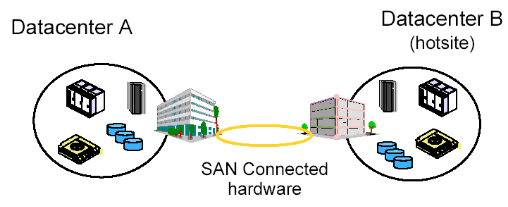
\includegraphics[width=8cm]{tier4.png}
\caption{Tier 4 \href{https://www.abzsol.com/cms/images/stories/pdf/business_continuity.pdf}{www.abzsol.com}}\end{figure}
Per SAP è previsto:
\begin{itemize}
\item backup off-site radicale ogni sei mesi su nastro  da conservare presso l'\textit{Offerente};
%\item backup off-site incrementale una volta al giorno su disco;
\item SAN connected hardware;
%\item backup off-site radicale ogni sei mesi su nastro;
%\item backup off-site incrementale una volta al giorno su disco;
%\item electronic vaulting per i dati più critici;
\item software di gestione Disaster Recovery (da stabilire in progettazione esecutiva - es: VMware che ben si integra con SAP e che supporta le SAN);
\item hot-site con installazione dei sistemi SAP (con relative librerie e documentazione);
\end{itemize}
Dovrà essere scelto un software di Disaster Recovery specifico per SAP, da integrare col software di gestione di DR degli altri sistemi presenti nella soluzione, con possibilità di personalizzazione di parametri quali la frequenza e la modalità di backup: la perdita di alcune ore di dati è ancora ammissibile, ma copie di tipo Point-in-Time (PIT) permettono con falicità backup con una frequenza più elevata rispetto al semplice trasferimento dei dati su nastro.
Quindi, anche se i dati potrebbero essere aggiornati nel peggiore dei casi alle 4 ore precedenti, i sistemi sostitutivi saranno già funzionanti.
Altri dati necessari per eseguire l'applicazione (librerie, documentazione, copie delle licenze software) vengono inviati anche al sito secondario attraverso il software di gestione del DR al momento della creazione della soluzione. Il software permetterà anche il monitoraggio e il controllo della situazione in ogni momento sia antecedente all'emergenza, sia in fase di emergenza, che di rientro.

\subsubsection{Fase di reazione all’emergenza}
Istruzioni operative del start-up di dettaglio verranno fornite in sede di progettazione esecutiva. Si cercherà di automatizzare al massimo ogni operazione tramite script automatici, di modo da minimizzare, per quanto possibile, l'intervento umano. 
Supponendo che strutture generali, infrastruttura e componenti hardware siano ripristinati, le procedure di recupero rispetteranno le seguenti linee guida generali:
\begin{itemize}
\item avvio dei sistemi nel sito secondario tramite software di gestione del DR;
\item lancio della riconfigurazione automatizzata delle risorse di rete;
\item controllo del corretto collegamento del sistema alla rete di produzione;
\item controllo del corretto ripristino dei sistemi operativi;
\item ripristino dei dati applicativi;
\item controllo del corretto ripristino della configurazione dei dati di sistema;
\item controllo del corretto ripristino del software applicativo;
\item lancio del testing automatizzato per la sicurezza;
\item lancio del testing automatizzato per le funzionalità di base del sistema;
\end{itemize}

\subsubsection{Fase di gestione dell’emergenza}
\begin{itemize}
\item L'amministrazione e monitoraggio dei sistemi di sostituzione per SAP viene affidato all'ing. X, e in secondo luogo al sig. XX.
\item Non è previsto che gli operatori sanitari, amministrativi, o che i tecnici debbano spostarsi fisicamente verso la struttura sostitutiva.
\item La situazione sarà sempre controllabile da remoto sia dall'Istituto che dalla \textit{nostra} azienda.
\item In caso di necessità è prevista la possibilità di mandare tecnici della \textit{nostra} azienda o professionisti esterni mandati da parte della nostra azienda.
\item Gli accessi si sistemi SAP dovranno essere controllati dal software di gestione di DR.
\item I dati creati in fase di gestione dell'emergenza devono essere memorizzati in un ambiente secondario, in modo da facilitarne il successivo restore.
\end{itemize}


%*************************************************************
\newpage
\subsection{Soluzione di Continuità per SISS}
\subsubsection{Interrelazioni con entità esterne all’Amministrazione}
I contratti in essere che vengono coinvolti sono:
\renewcommand \arraystretch{1,5}
\begin{longtable}{c c c}
\toprule
\textbf{Contratto in Essere} & \textbf{Fornitore} & \textbf{Produttore} \\
\toprule
	Contratto unico per fornitura servizi IT & Offerente & Offerente \\
\bottomrule
\caption{Contratti SISS}
\end{longtable}
Non si rilevano necessità di effettuare variazioni contrattuali ai contratti sopracitati.
\subsubsection{Assunzioni ai fini del progetto didattico}
Ai fini del progetto didattico,si suppone che i dati che vengono creati all'interno dell'Istituto siano memorizzati nelle repository centrali oppure che vengano spediti ai server centrali SISS, e che quindi nella \textit{"Porta Applicativa"} esistano server, routers, firewall e il software atti all'invio e alla ricezione di dati da e verso i DB centrali SISS, senza vere e proprie strutture ospitanti dati al suo interno. Si specifica che, anche in caso questa assunzione sia scorretta, sarebbe stata ipotizzata una soluzione simile a quella indicata successivamente per i servizi SAP.
\subsubsection{Soluzione}
Per SISS è prevista l'adozione del Tier 4 con:
\begin{itemize}
\item software di gestione Disaster Recovery (da stabilire in progettazione esecutiva es: Tivoli IBM);
\item warm-site con
  \begin{itemize}
  \item installazione della \textit{Porta Applicativa SISS} (con relative librerie e documentazione);
  \item cache predisposta per la memorizzazione temporanea delle richieste verso i sistemi centrali SISS;
  \end{itemize}
\end{itemize}
Saranno presenti le attrezzature hardware dotate di connessione e pre-configurate. In caso di emergenza verrà come prima cosa avviata la cache temporanea, che servirà per la presa in carico delle richieste verso i sistemi centrali SISS. Queste richieste verranno gestite una volta che il servizio sostitutivo sarà attivo. L'attivazione della soluzione sostitutiva nel frattempo sarà gestita attraverso il software di gestione di DR prescelto.
\\
Altri dati necessari per eseguire l'applicazione (librerie, documentazione, copie delle licenze software) vengono inviati anche al sito secondario attraverso il software di gestione del DR al momento della creazione della soluzione. Il software permetterà anche il monitoraggio e il controllo della situazione in ogni momento sia antecedente all'emergenza, sia in fase di emergenza, che di rientro.

\subsubsection{Fase di reazione all’emergenza}
Istruzioni operative del start-up di dettaglio verranno fornite in sede di progettazione esecutiva. Si cercherà di automatizzare al massimo ogni operazione tramite script automatici, di modo da minimizzare, per quanto possibile, l'intervento umano. 
Supponendo che strutture generali, infrastruttura e componenti hardware siano ripristinati, le procedure di recupero rispetteranno le seguenti linee guida generali:
\begin{itemize}
\item avvio della cache temporanea tramite software di gestione del DR;
\item avvio dei sistemi sostitutivi tramite software di gestione del DR;
\item lancio della riconfigurazione automatizzata delle risorse di rete;
\item collegamento del sistema alla rete di produzione;
\item ripristino dei sistemi operativi;
\item lancio del testing automatizzato per la sicurezza;
\item lancio del testing automatizzato per le funzionalità di base del sistema;
\item gestione delle richieste accodate nella cache temporanea;
\end{itemize}

\subsubsection{Fase di gestione dell’emergenza}
\begin{itemize}
\item L'amministrazione e monitoraggio dei sistemi di sostituzione per la \textit{Porta Applicativa SISS} viene affidato all'ing. X, e in secondo luogo al sig. XX.
\item Non è previsto che gli operatori sanitari, amministrativi, o che i tecnici debbano spostarsi fisicamente verso la struttura sostitutiva.
\item La situazione sarà sempre controllabile da remoto sia dall'Istituto che dalla \textit{nostra} azienda.
\item In caso di necessità è prevista la possibilità di mandare tecnici della \textit{nostra} azienda o professionisti esterni mandati da parte della nostra azienda.
\item Gli accessi si sistemi appartenenti alla \textit{Porta Applicativa SISS} dovranno essere controllati dal software di gestione di DR.
\end{itemize}

%***************************************************

\newpage
\subsection{Fase di ritorno alla normalità}
\label{rientro}
Il software di gestione di DR deve gestire in modo più automatizzato possibile tutte le operazioni di rientro dalla situazione di emergenza. In particolare ci si aspetta che i dati creati in fase di gestione dell'emergenza saranno trasferiti in fase di  verso l'Istituto utilizzando procedure automatizzate.
Istruzioni operative del restore di dettaglio verranno fornite in sede di progettazione esecutiva. Supponendo che le funzioni di supporto dell'infrastruttura (alimentazione,  telecomunicazioni, strutture fisiche e hardware) siano stati correttamente riportati alla normalità, le procedue di restore rispetteranno le seguenti linee guida generali:
\begin{itemize}
\item controllo della corretta installazione dell'hardware;
\item ripristino del software di sistema;
\item ripristino del software applicativo;
\item ripristino dei dati sui sistemi di produzione;
\item controllo del corretto ripristino della configurazione dei dati di sistema;
\item lancio della riconfigurazione automatizzata delle risorse di rete;
\item avvio dei sistemi primari;
\item lancio del testing automatizzato per la sicurezza;
\item lancio del testing automatizzato per le funzionalità di base del sistema;
\item test per le funzionalità non di base del sistema;
\item arresto delle operazioni di emergenza;
\item reset e riconfigurazione del software di gestione del DR;
\item reset e riconfigurazione dei sistemi secondari.
\end{itemize}

Una volta che l'infrastruttura, la rete, i sistemi, le applicazioni e le interfacce sono stati testati per la produzione, il sito primario torna allo stato ordinario e il sito secondario viene riconfigurato di modo che sia pronto per reagire a un'eventuale futuro stato di emergenza. Infine le misure di emergenza verranno riviste in un ottica di miglioramento, come descritto in \textit{Operational Management} in \ref{opmgmt}. Entro un mese dal rientro della situazione di emergenza deve essere stilata la reportistica apposita contenente:
\begin{itemize}
\item descrizione dell'emergenza
\item analisi dei danni;
\item report attivazione gestione e rientro;
\item descrizione test di verifica rientro.
\end{itemize}















































%*******************************************************
\newpage
\section{Operational Management}
\label{opmgmt}
Una volta che l'implementazione e la pianificazione sono completate è necessario garantire che il processo sia mantenuto come parte del normale business.
\subsection{Education and Awareness} Tutto l'Istituto e in modo particolare i dipartimenti IT sono chiamati alla piena comprensione delle motivazioni che spingono verso l'adozione di misure di Continuità, in modo che siano al corrente delle implicazioni della Continuity nel loro lavoro quotidiano.
A tale scopo l'IT SC Manager organizzarà una volta all'anno nel mese di XX un seminario della durata di due ore.
\subsection{Formazione}
È importante garantire che il personale IT sia sempre competente e autonomo per quanto riguarda la Continuità. E' necessario quindi:
\begin{itemize}
\item stendere una documentazione appropriata che descriva la soluzione di continuità comprendendo ogni attività che i membri del team devono fare, le modalità e le tempistiche, assieme ai ruoli che devono assumere e le loro responsabilità;
\item tenere seminari sia di carattere teorico che pratico per assicurare la piena comprensione dei contenuti: sono previste 24 ore di formazione al termine del progetto e 8 ore di formazione ogni anno. Le modalità saranno concordate nel dettaglio in fase di progettazione esecutiva.
\item tenere verifiche annuali al termine dei seminari. Le modalità saranno concordate nel dettaglio in fase di progettazione esecutiva.
\end{itemize}
\subsection{Modalità di esecuzione dei test periodici}
Per quanto attiene ai test sono possibili varie modalità di test: 
\begin{itemize}
\item \textbf{checklist}: viene effettuata una semplice verifica dell’effettiva disponibilità di tutto quanto si renderebbe necessario in caso di emergenza, basandosi su una cheklist, come descritto nella sezione successiva;
\item \textbf{test  degli  impianti  e  delle  risorse con sistemi primari attivi: } Il Responsabile per la Continuità avvierà l'esecuzione della simulazione che coinvolgerà l'attivazione  delle  risorse  fisiche secondarie, senza la disattivazione delle risorse primarie. Durante la simulazione per ognuna delle fasi, vengono eseguite le attività previste nel corrente piano e il Responsabile monitorerà attentamente l'esecuzione fino a quando i servizi non saranno tornati alla normalità.
\item \textbf{test  degli  impianti  e  delle  risorse con disattivazione dei sistemi primari:}  viene effettuata una simulazione che coinvolga l’effettiva 
attivazione  delle  risorse  fisiche  e  IT e, per ognuna delle fasi, vengono eseguite le attività previste nel corrente piano e una verifica dell'uso delle corrette procedure. Per Aurora è previsto che, durante la disattivazione, venga usato l'ambiente di test. Il Responsabile per la Continuità avvierà l'esecuzione del piano e monitorerà attentamente l'esecuzione fino a quando i servizi non saranno tornati alla normalità. Un  test  di  questo  tipo  richiede  una  attenta  predisposizione  e  un  sensibile impegno  per  il  personale,  ma  garantisce  la  reale  verifica  della  soluzione  di  continuità  del  PCO  ICT. 
\end{itemize}
In caso di errori o incompletezze, il piano viene rivisitato come descritto nella sezione seguente.
I test vanno eseguiti dopo ogni eventuale calamità che dovesse attivare qualche soluzione di emergenza.
\subsubsection{Frequenza e finestre per i test}
\begin{itemize}
\item simulazione in attivo: 1 volta all'anno - durante il mese di MeseX dalle hh:mm alle hh:mm, senza preavviso del personale;
\item checklist: 1 volta all'anno - entro un mese dopo la simulazione in attivo;
\item simulazione con disattivazione: 1 volta all'anno da concordare entro il GG Mese+1, e da effettuare con un preavviso di almeno 1 mese.
\end{itemize}
E' necessario un documento scritto o elettronico che attesti l'esecuzione di ogni test.
\subsection{Modalità di revisione e adeguamento del piano}
Il Piano di Continuità ICT non è un documento statico e, pertanto, è necessario pianificare, all’interno del PCO ICT stesso le modalità di revisione e aggiornamento. Sarà il SC team ad effettuare la revisione, guidato dall'IT SC Manager.
La modalità di revisione è scelta è la \textit{checklist}, un elenco di punti da controllare da predisporre nel dettaglio in fase di progettazione esecutiva, ma che in linea di massima conterrà i punti relativi a:
  \begin{itemize}
  \item modifiche nella composizione della/e struttura/e organizzava/e preposte alla gestione della continuità operativa ICT; 
  \item modifiche nei dati personali e/o di reperibilità;
  \item modifiche dei fornitori e/o del contratto assicurativo; 
  \item modifiche dei servizi o delle applicazioni software (aggiunta o eliminazione di applicazioni, 
  variazioni nella criticità/priorità delle applicazioni); 
  \item modifiche nell’hardware e/o nella rete;
  \item modifiche nella logistica; 
  \item stipula di nuovi contratti. 
  \end{itemize}
  Vista la natura della checklist, il Service Continuity Team sarà chiamato a collaborare con il Change Management per una armonizzazione di quanto descritto tra i due processi di Change e Continuity. In particolare ad ogni cambiamento che avverrà a uno dei punti stabiliti nella check-list è previsto che sia il Change Management che in maniera attiva informi il Service Continuity Team. Al termine di ogni revisione del presente documento, le Change opportune devono essere gestite assieme al CAB.
Il corrente piano viene rivisitato secondo la modalità descritta dal Comitato di Revisione e approvato dal Responsabile della Continuità ICT.            
% !TEX encoding = UTF-8
% !TEX TS-program = pdflatex
% !TEX root = ../tesi.tex
% !TEX spellcheck = it-IT

%*********************************************************
\chapter{SLA Management}
\begin{flushright}
\textit{a cura di \large{Marco Casagrande}}
\end{flushright}
\label{cap:slamanagement}
%**********************************************************

\section{Panoramica generale}

\subsection{Consegna}

Pianificazione ed organizzazione del processo di SLA Management; secondo quanto indicato nel Capitolato Tecnico dell'Azienda Ospedaliera Gaetano Pini, sezione 5.1.4.5 - Misurazione dei livelli di Servizio (SLA Management):
\\

\textit{"Il Service Level Agreement (SLA) è un accordo tra un utente e un fornitore di un servizio che definisce la natura del servizio fornito e stabilisce un insieme di parametri da utilizzare per misurare il livello del servizio erogato. L’accordo può essere molto dettagliato ed includere la definizione di ruoli, delle responsabilità e dei termini da cui far decorrere le penali. 
\\ \\
La Gestione dei Livelli di Servizio (SLA Management) è il processo che riguarda il governo dei Livelli di Servizio richiesti nel presente capitolato e/o proposti nell’Offerta Tecnica e riportati nel Contratto. Il processo focalizza gli aspetti peculiari della preparazione (e/o rinnovo), registrazione, e controllo dei Livelli di Servizio contrattuali.
\\ \\
L’Istituto chiede ai concorrenti di fornire i servizi di gestione in questa ottica di SLA. Pertanto l’offerente dovrà organizzare il servizio con l’obiettivo di poter documentarne la rispondenza a dei parametri (livelli) precedentemente definiti, in modo condiviso e concorde, con l’Istituto. L’offerente dovrà descrivere le attività di SLA management di cui si farà carico durante la gestione, indicando anche gli strumenti che intende utilizzare per registrare e documentare il livelli di servizio.
\\ \\
L’offerente deve quindi proporre un sistema informativo dedicato alla gestione degli SLA, “lo SLA Manager”, che ha quindi come obiettivo finale l’esposizione dello stato effettivo del servizio erogato. Tutto ciò, ponendo in relazione i livelli di servizio erogati con le norme che regolano contrattualmente l’erogazione del servizio in generale, attraverso indicatori oggettivamente misurabili, esplicitamente richiesti dall’Istituto e/o proposti dall’offerente sulla base del proprio know how.
\\ \\
L’Istituto richiede che, tramite opportune funzionalità, si possa verificare in qualsiasi momento, in modo autonomo e disgiunto (da parte dell’Istituto o dell’offerente), lo stato del servizio e di conseguenza il rispetto dei termini contrattuali."}

\subsection{Definizione degli obiettivi}

I punti chiave del processo di SLA Management, estrapolati dalle richieste presenti nel capitolato sono:

\begin{itemize}
	\item la definizione delle attività di preparazione, rinnovo, registrazione e controllo degli SLAs;
    \item la definizione degli strumenti necessari e di un sistema informativo a supporto del processo.
\end{itemize}

Il processo di Service Level Management, definito nel framework ITIL, è estremamente affine a quanto richiesto per il processo di SLA Management. Lo sfrutteremo dunque come base di partenza.

\begin{figure}[H]
\centering
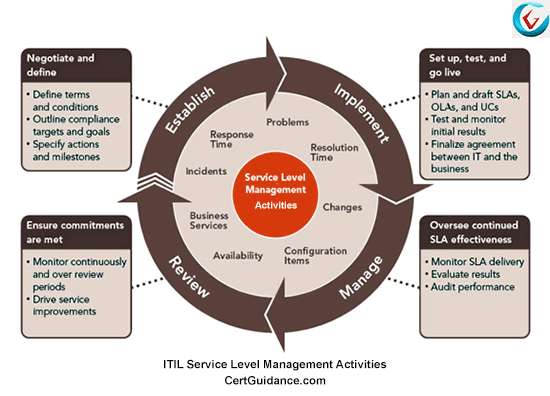
\includegraphics[width=30em]{immagini/sla/slmdiagram.png}
\caption{Diagramma ITIL del processo di Service Level Management}
\end{figure}

Il processo di Service Level Management si occupa di:

\begin{itemize}
	\item definire ed organizzare un Service Catalogue dei servizi erogati dal fornitore;
	\item progettare i Service Level Requirements per i nuovi servizi;
    \item trasformare gli SRL in Service Level Agreements;
    \item definire gli Operational Level Agreements e gli Underpinning Contracts necessari a garantire gli SLAs concordati;
    \item monitorare le performance di SLAs, OLAs, UCs e produrre report ad intervalli regolari;
    \item condurre indagini e review sulla qualità e sui possibili miglioramenti dei servizi rispetto agli SLAs, secondo i Service Improvement Programs;
    \item gestire i rapporti con i clienti per garantirne la soddisfazione.
\end{itemize}

Il processo di Service Level Management ospita quattro sotto-processi:

\begin{itemize}
	\item Maintenance of the SLM Framework, con lo scopo di progettare e mantenere il Customer Agreement Portfolio e fornire i template dei documenti necessari al processo di SLM;
    \item Identification of Service Requirements, con lo scopo di catturare i desideri dei clienti per dei nuovi servizi o per delle modifiche a quelli preesistenti;
    \item Agreements Sign-Off and Service Activation, con lo scopo di finalizzare le sottoscrizioni ai contratti di SLAs, OLAs, UCs e verificare i Service Acceptance Criteria;
    \item Service Level Monitoring and Reporting, con lo scopo di monitorare le prestazioni dei servizi rispetto a quelle concordate e diffondere i Service Level Reports.
\end{itemize}

Le richieste presentate nel Capitolato Tecnico rispetto al processo di SLA Management trovano corrispondenza nel processo ITIL di Service Level Management. Quest'ultimo pone inoltre obiettivi di qualità ed enfasi sulle relazioni con i clienti, entrambi non espressamente richiesti nel Capitolato Tecnico. Durante l'implementazione del nuovo processo di SLA Management attribuiremo una priorità inferiore a tali aspetti, in quanto ritenuti meno interessanti dal cliente.

\subsection{Fonti}

Vengono qui riportate le fonti cui ho attinto per conoscenze ed ispirazione allo scopo di redigere il capitolo SLA Management:

\begin{itemize}
	\item \href{http://www.netadm.it/admsys_2018/admsys.htm}{Corso di Amministrazione di Sistema 2017/2018}, in particolare le slide delle lezioni;
    \item \href{https://wiki.en.it-processmaps.com/index.php/Main_Page}{IT Process Wiki}, per qualsiasi approfondimento legato ai processi ITIL ma anche alle checklist per i documenti SLA, OLA ed UC;
    \item \href{https://www.teamquest.com/files/6614/2049/9759/itil4.pdf}{TeamQuest}, per la descrizione approfondita sull'implementazione del processo ITIL di Servel Level Management;
    \item \href{https://www.hci-itil.com/ITIL_v3/docs/3792_itil_ebook_1.pdf}{HCI-ITIL}, per la descrizione approfondita sull'implementazione del processo ITIL di Servel Level Management;
    \item \href{https://www.theitsmhub.com.au/wp-content/uploads/2014/12/A-Practical-Approach-to-Implementing-Service-Level-Management.pdf}{Pink Elephant}, per la descrizione approfondita sull'implementazione del processo ITIL di Servel Level Management;
        \item \href{https://www.pinkelephant.com/uploadedFiles/Content/ResourceCenter/PinkPapers/ImplementingServiceLevelManagement.pdf}{Pink Elephant}, per un ulteriore punto di vista sul processo ITIL di Servel Level Management;
    \item \href{https://wiki.scn.sap.com/wiki/display/SAPITSM}{SAP Community Wiki}, in particolare i vari post riguardo all'implementazione di processi ITIL tramite SAP Solution Manager;
    \item \href{https://support.sap.com/en/index.html}{SAP Support Portal}, per l'approfondimento riguardo allo strumento software SAP Solution Manager;
    \item \href{https://help.sap.com/viewer/index}{SAP Help Portal}, per l'approfondimento riguardo allo strumento software SAP Solution Manager;
    \item \href{https://tsd.gmu.edu/policies/SLAs/}{George Mason University}, per un template di SLA;
    \item \href{https://tsd.gmu.edu/policies/olas.cfm}{George Mason University}, per un template di OLA;
    \item \href{https://its.ucsc.edu/itsm/servicemgmt.html#definition}{UC Santa Cruz}, per un template di SLA;
    \item \href{https://its.ucsc.edu/itsm/servicemgmt.html#definition}{UC Santa Cruz}, per un template di OLA;
    \item \href{http://www.axia-consulting.co.uk/html/sla_metrics.html}{Axia-Consulting}, per informazioni sulle metriche degli SLAs;
    \item \href{http://www.slatemplate.com/}{ SLA Template.com}, per un template di SLA;
    \item \href{https://www.certguidance.com/topics/itil-foundation/}{CertGuidance}, per alcuni articoli e l'immagine del diagramma SLM;
    \item \href{https://www.uptrends.com/}{Uptrends}, per l'approfondimento riguardo allo strumento software Uptrends;
    \item \href{https://www.happyfox.com/}{happyfox}, come possibile strumento informatico;
    \item \href{https://www.webhelpdesk.com/help-desk-software/sla-management-monitoring-reports}{web help desk}, come possibile strumento informatico;
    \item \href{https://www.dotcom-monitor.com/web-performance-reports/sla-management/}{dotcom-monitor}, come possibile strumento informatico;
    \item \href{https://www.idera.com/it-infrastructure-management-and-monitoring/sla-management-tools}{IDERA}, come possibile strumento informatico.
\end{itemize}

\section{Pianificazione delle attività}

Riportiamo per comodità di consultazione il piano dei servizi di gestione ed i vincoli temporali, come presentati nel Capitolato Tecnico alla sezione 5.2.1 - Piano dei servizi di gestione richiesti ed alla sezione 5.2.1.2 - Vincoli Temporali.

\begin{figure}[H]
\centering
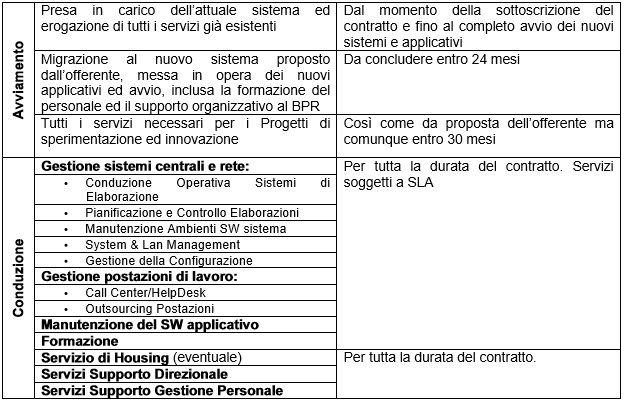
\includegraphics[width=30em]{immagini/sla/planning.png}
\caption{Piano dei servizi di gestione}
\end{figure}

\begin{figure}[H]
\centering
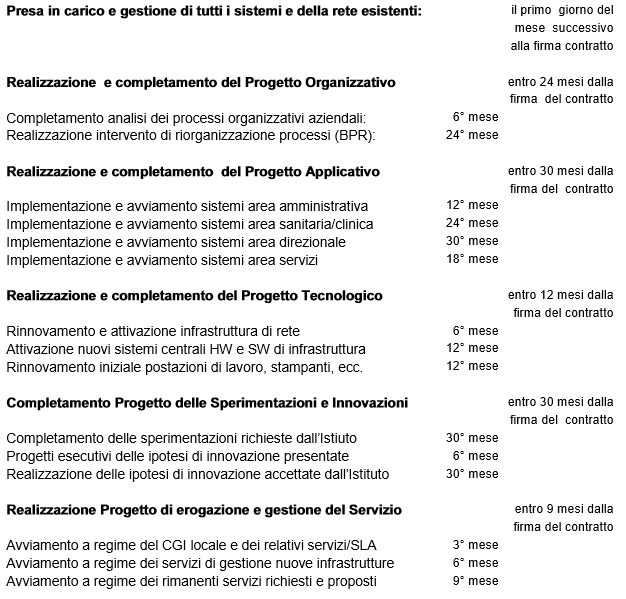
\includegraphics[width=30em]{immagini/sla/timeconstraints.png}
\caption{Vincoli temporali}
\end{figure}

\subsection{Pianificazione delle attività di avviamento}

La seguente tabella illustra le attività di avviamento previste, il periodo di tempo massimo per il loro svolgimento (considerato a partire dalla firma del contratto) e l'obiettivo di riferimento:

\begin{center}
    \begin{tabular}{ | p{4cm} | p{5cm} | l | }
    \hline
    Attività & Obiettivo & Periodo \\ 
    \hline
    
    Formazione & Favorire la comunicazione con i manager tramite una formazione intensiva riguardo ITIL & Entro un mese \\ 
    \hline
    Identificazione dei requisiti di business & Uniformare la visione del business con i processi che coinvolgono il nuovo dipartimento IT & Entro un mese \\ 
    \hline
    Analisi dello stato attuale & Comprendere le caratteristiche e le dinamiche dell'attuale dipartimento IT & Entro due mesi \\
    \hline
    Scelta dei responsabili del processo di SLA Management & Nominare i responsabili e affidare loro le attività riguardanti lo SLA Management & Entro due mesi \\
    \hline
    Implementazione del processo di SLA Management per il Centro di Gestione Integrato & Delineare una bozza funzionante del processo di SLA Management (solo per i servizi necessari al CGI) ed inserirlo tra i processi del nuovo dipartimento IT & Entro tre mesi \\
    \hline
    Gap analysis & Localizzare e risolvere dei gap trovati negli attuali processi che coinvolgono il dipartimento IT & Entro tre mesi \\
    \hline
    Creazione del Service Catalogue & Individuare i servizi IT richiesti ed inserirli nel Service Catalogue & Entro quattro mesi \\
    \hline
    Valutazione degli SLAs, OLAs ed UCs preesistenti & Documentare e monitorare gli SLAs, OLAs ed UCs preesistenti ed in seguito valutarli rispetto alle richieste presenti nel Capitolato Tecnico & Entro cinque mesi \\
    \hline
    Definizione di metriche e KPIs & Formulare metriche e KPIs aggiornati alle nuove richieste e necessità del business & Entro sei mesi \\
    \hline
    Definizione delle modalità di monitoraggio & Istituire gli strumenti per il monitoraggio di metriche e KPIs aggiornati & Entro sei mesi \\
    \hline
    Implementazione del nuovo processo di SLA Management & Finalizzare il processo di SLA Management ed inserirlo tra i processi del nuovo dipartimento IT & Entro otto mesi \\
    \hline
    Inserimento di sperimentazioni e innovazioni nello SLA Management & Estendere il processo di SLA Management ai servizi necessari per il progetto delle sperimentazioni e innovazioni presentato & Entro dieci mesi \\
    \hline
    
    \end{tabular}
\end{center}

\subsection{Pianificazione delle attività di conduzione}

Le attività di conduzione sono:

\begin{itemize}
	\item Establish - Ridefinizione del processo;
    \item Implement - Implementazione dei nuovi SLAs;
    \item Manage - Monitoraggio del processo;
    \item Review - Revisione del processo.
\end{itemize}

%**********************************************************

\section{Attività di avviamento}

\subsection{Formazione}

La formazione necessaria al nuovo processo di SLA Management fa parte dell'introduzione al framework ITIL nell'Azienda Ospedaliera. Sebbene il nuovo dipartimento IT sarà composto da personale qualificato (sia interno che esterno) a nostra discrezione, la logica ITIL non può maturare senza un'espansione verso i dipendenti dell'Istituto stesso. 
\\
Riteniamo indispensabile programmare un corso di formazione sul framework ITIL coinvolgendo ogni manager che lavorerà a contatto con il nuovo dipartimento IT, e sotto gli stessi presupposti lo riteniamo consigliabile anche per gli altri dipendenti. La cooperazione con i manager è fondamentale per ottenere una chiara visione del business e soddisfarne le richieste. La cooperazione con i dipendenti invece è fondamentale per implementare correttamente i processi ed ottenere risultati a livello operativo. L'istituzione di un linguaggio comune costituisce la garanzia a lungo termine per un rapporto virtuoso tra Azienda Ospedaliera e nuovo dipartimento IT, di cui il Capitolato Tecnico costituisce una mera base di partenza.
\\
Dal lato opposto è fondamentale che il business comprenda i vantaggi dell'adozione del framework ITIL, ed in particolare il rigido rispetto degli SLAs così da pubblicizzarli e metterli pienamente a frutto. Il nostro scopo come organizzazione non è solo l'erogazione dei servizi richiesti, ma anche l'inquadramento dei processi preesistenti all'interno dell'Istituto in un'ottica di efficacia, efficienza e miglioramento continuo.
\\ \\
Per l'attività di formazione prevediamo la partecipazione a seminari collettivi al livello ITIL Foundations di figure manageriali e dipendenti scelti. I seminari saranno organizzati da nostri esperti provvisti di certificazione ufficiale.

\subsection{Identificazione dei requisiti di business}

Come accennato nella sezione precedente, il Capitolato Tecnico costituisce una buona base di partenza per identificare i requisiti di business ma è impossibile catturarne la visione completa da un singolo documento. In particolare, evidenzieremo i requisiti di business riguardanti il nuovo processo di SLA Management.
\\
Nel Capitolato Tecnico, alla sezione 5.3 - Definizione Servizi e SLA, si possono consultare i Service Level Requirements rilevati dall'Azienda Ospedaliera. Nel documento sono indicati come Service Level Agreements, ma ci permettiamo di correggere la terminologia. Infatti, gli SLR sono le richieste avanzate dal cliente al fornitore che descrivono le aspettative riguardanti il servizio erogato, esattamente ciò che risulta descritto nel documento. Per definire degli SLAs ottimali è necessario confermare correttezza e completezza degli SRLs già documentati.
\\ \\
Per l'attività di identificazione dei requisiti di business prevediamo di effettuare visite, interviste e riunioni che coinvolgano il personale (principalmente figure manageriali) e le unità di business a stretto contatto con il dipartimento IT.

\subsection{Analisi dello stato attuale}

Allo scopo di pianificare correttamente processi ed attività, riteniamo vitale stabilire lo stato attuale dell'Istituto, in particolare nel settore IT. I fattori più influenti che valuteremo sono:

\begin{itemize}
	\item lo stato dei software (software generici, applicativi specifici dell'Azienda Ospedaliera, criteri e modalità di accesso e download ai software...);
    \item lo stato delle attrezzature hardware (server, desktop, router, periferiche, cavi, giacenze in magazzino...);
    \item la capacità di monitoraggio delle prestazioni attuali (misurazioni sulla connessione internet, misurazioni sulle risposte degli applicativi...);
    \item lo stato del personale ospedaliero (disponibilità fisica e temporale, competenze individuali...);
    \item la presenza di dinamiche interne peculiari (rispetto di procedure e processi, metodi di generazione e trasporto di documentazione, gestione delle emergenze...);
    \item la disponibilità e le caratteristiche degli spazi per il nuovo dipartimento IT (Centro Elaborazione Dati - CED, networking tra le stanze...);
    \item le limitazioni geografiche tra stanze, piani ed edifici (presenza di ostacoli, limitazioni dovute a macchinari medici, distanza geografica elevata...);
    \item la percezione dei servizi erogati dall'Azienda Ospedaliera (dal punto di vista di business/dipendenti/pazienti...);
    \item il grado di maturità del processo preesistente che si occupa degli SLAs (Capability Maturity Model).
\end{itemize}

Per l'attività di analisi dello stato attuale prevediamo la consultazione di documenti preesistenti e l'organizzazione di visite, interviste e riunioni che coinvolgano il personale (principalmente figure manageriali) e le unità di business a stretto contatto con il dipartimento IT.

\subsection{Scelta dei responsabili del processo di SLA Management}

L'assegnazione delle responsabilità ad una persona fisica apre una finestra di dialogo diretto con l'Istituto. Tre sono i ruoli principali che abbiamo individuato:

\begin{itemize}
	\item un Service Level Manager (Process Owner);
    \item almeno un Service Owner;
    \item almeno un Customer Representative.
\end{itemize}

Il Service Level Manager è responsabile della stipulazione e dell'adempimento degli SLAs. Si occupa di garantire la conformità del processo di SLA Management, degli OLAs e degli Underpinning Contracts rispetto agli SLAs. Inoltre, si occupa del monitoraggio e dei documenti di report per gli SLAs.
\\
Il Service Owner è responsabile dell'erogazione di un determinato servizio e spesso ricopre un lato tecnico. Il numero di Service Owners sarà deciso dalla nostra organizzazione in base alle necessità verso la gestione dei servizi preesistenti. Ciascun Service Owner prenderà in carico uno o più servizi e valuterà le attuali prestazioni, proponendo un piano per gli sviluppi futuri (dismissione, delega ad un service provider esterno, erogazione del servizio internamente...).
\\
Il Customer Representative è il rappresentante degli interessi del cliente (in questo caso l'Azienda Ospedaliera). Si occupa di comunicare le aspettative del business verso lo SLA Management grazie alla sua esperienza lavorativa ed alla sua conoscenza del settore ospedaliero. Il numero di Customer Representatives è a discrezione dell'Azienda Ospedaliera, ma consigliamo l'assegnazione di almeno uno di essi così da addolcire l'insediamento del nuovo dipartimento IT.
\\
Per l'attività di scelta dei responsabili del processo di SLA Management prevediamo dunque l'assegnazione dei ruoli di Service Level Manager e Service Owner internamente alla nostra organizzazione, e l'assegnazione del ruolo di Customer Representative internamente all'Azienda Ospedaliera.

\subsection{Implementazione del processo di SLA Management per il Centro di Gestione Integrato}

I vincoli temporali presentati nel Capitolato Tecnico pianificano l'avviamento a regime del Centro di Gestione Integrato locale e di relativi servizi/SLAs entro il terzo mese dopo la firma del contratto. Al fine di rispettarli, la nostra organizzazione definirà una bozza per il nuovo processo di SLA Management riguardante solo i servizi necessari al CGI. La finalizzazione del processo di SLA Management richiede un'analisi più approfondita di quella conducibile in soli tre mesi: questa attività quindi formulerà una versione parziale e temporanea del processo, da estendere e perfezionare successivamente durante l'attività di implementazione del nuovo processo di SLA Management.
\\
Per l'attività di implementazione del processo di SLA Management per il Centro di Gestione Integrato prevediamo l'istituzione di un team di esperti, stabilito internamente alla nostra organizzazione, e dedicato esclusivamente a questa attività.

\subsection{Gap analysis}

La gap analysis è uno strumento manageriale per confrontare le attuali performance del business con quelle potenziali. Con il termine gap si intende l'allocazione non ottimale delle risorse. Approfittando delle circostanze di rinnovamento totale del dipartimento IT, accorceremo la distanza di prospettive tra esso ed il business dell'Istituto. Processi inefficaci, procedure obsolete e sprechi di risorse influiscono enormemente sulle performance dei servizi IT, in particolare la reattività alle segnalazioni.
\\
Per l'attività di gap analysis prevediamo l'istituzione di un team di esperti che abbia a disposizione le informazioni ricavate dall'attività di analisi dello stato attuale. Tale team sarà composto sia da nostri esperti sia da esponenti dell'Azienda Ospedaliera, così da condurre a risultati quanto più accurati possibili.

\subsection{Creazione del Service Catalogue}

Il Service Catalogue è un documento contenente l'elenco dettagliato di tutti i servizi di un fornitore visibili ai clienti. Comprende i servizi di terze parti, in quanto la nostra organizzazione ha la responsabilità riguardo alla loro erogazione ed ai rapporti con i rispettivi fornitori. La prima versione del Service Catalogue comprenderà solo i servizi attualmente erogati, reperibili nel Capitolato Tecnico, sezione 2.2 - Sistemi applicativi esistenti e descrizione del contesto. Formuleremo versioni successive durante le normali attività di conduzione del processo di SLA Management.
\\
Per l'attività di creazione del Service Catalogue prevediamo l'istituzione di un team di esperti, stabilito internamente alla nostra organizzazione.

\subsection{Valutazione degli SLAs, OLAs ed UCs preesistenti}

Gli attuali servizi erogati all'Istituto, qualunque siano i rispettivi fornitori, dovrebbero rispettare determinati SLAs che possibilmente saranno a loro volta alimentati da OLAs ed UCs con terze parti. Valutare le condizioni attuali dei servizi è imperativo per garantire gli SLAs richiesti nel Capitolato Tecnico. Qualora uno o più servizi non rispettassero i nuovi SLAs mantenendo gli attuali contratti, la nostra organizzazione si farà carico di risolvere la situazione.
\\
Per l'attività di valutazione degli SLAs, OLAs ed UCs preesistenti prevediamo l'istituzione di un team di esperti, stabilito internamente alla nostra organizzazione.

\subsection{Definizione di metriche e KPIs}

I KPIs sono quantità misurabili di natura strategica che riflettono la vicinanza del business ai propri obiettivi. In quanto tali, la scelta di essi è strettamente influenzata dalla visione del business; di cui saremo a conoscenza grazie alle attività di identificazione dei requisiti di business e di gap analysis.
\\
Le metriche sono quantità misurabili di natura tattica che riflettono le performance di processi/attività. In quanti tali, la scelta di esse è strettamente influenzata dal processo/attività di riferimento. Nell'ambito del processo di SLA Management, le metriche provengono dagli SLAs richiesti nel Capitolato Tecnico nonchè dagli OLAs ed UCs preesistenti; di cui siamo a conoscenza grazie alle attività di analisi dello stato attuale, di creazione del Service Catalogue e di valutazione degli SLAs, OLAs ed UCs preesistenti.
\\
Per l'attività di definizione di metriche e KPIs prevediamo l'istituzione di un team di esperti, stabilito internamente alla nostra organizzazione.

\subsection{Definizione delle modalità di monitoraggio}

Le modalità di monitoraggio dipendono strettamente dalle metriche e dai KPIs stabiliti per il processo di SLA Management. La chiara definizione di metriche e KPIs dunque è un prerequisito fondamentale per questa attività. Il monitoraggio deve tener conto anche degli elementi software ed hardware a disposizione, così da fornire la soluzione ottimale con le risorse attualmente a disposizione. Redigeremo un elenco delle possibli migliorie e criticità, con una valutazione riguardo a costi e benefici.
\\
Per l'attività di definizione delle modalità di monitoraggio prevediamo l'istituzione di un team di esperti, stabilito internamente alla nostra organizzazione.

\subsection{Implementazione del nuovo processo di SLA Management}

A partire dai processi interni all'Istituto, in particolare quelli che si interfacceranno con il nuovo dipartimento IT, applicheremo gradualmente i cambiamenti dettati dalla logica ITIL e dal business. Al termine di questa lenta metamorfosi, i processi saranno stati completamente rinnovati e riorganizzati.
\\
Il processo di SLA Management entrerà nel pieno delle attività di conduzione seguendo uno pseudociclo (Establish, Implement, Manage e Review). Istanzieremo i sottoprocessi dello SLA Management (Maintenance of the SLM Framework, Identification of Service Requirements, Agreements Sign-Off and Service Activation e Service Level Monitoring and Reporting) e abiliteremo operativamente il rispettivo personale. Sostituiremo la versione temporanea del processo di SLA Management ristretta al Centro di Gestione Integrato con la versione completa, rielaborata con più cura durante i mesi trascorsi.
\\
Per l'attività di definizione delle modalità di monitoraggio prevediamo l'istituzione di un team di esperti, stabilito internamente alla nostra organizzazione, e dedicato esclusivamente a questa attività.

\subsection{Inserimento di sperimentazioni e innovazioni nello SLA Management}

I vincoli temporali presentati nel Capitolato Tecnico prevedono la presentazione dei progetti esecutivi delle ipotesi di innovazione presentate entro il sesto mese dalla firma del contratto. Considerato ciò, preferiamo finalizzare il nuovo processo di SLA Management e verificarne le performance prima di dedicarci alle sperimentazioni ed innovazioni. Una volta delineati i progetti esecutivi delle ipotesi di innovazione, condurremo analisi e valutazioni del loro possibile impatto sui processi del nuovo dipartimento IT, prima di procedere con l'inserimento nel processo di SLA Management.
\\
Per l'attività di inserimento di sperimentazioni e innovazioni nello SLA Management prevediamo l'utilizzo di risorse già previste per le normali attività di conduzione dal processo di SLA Management.

%**********************************************************

\section{Attività di conduzione}

\subsection{Establish - Ridefinizione del processo}

Durante l'attività di Establish (e solo durante essa) apportiamo eventuali cambiamenti al processo, approvati da una precedente attività di Review. Fattori scatenanti possono essere variazioni degli SLAs, delle strategie di business, dei Service Improvement Programs oppure semplicemente ottimizzazioni a livello operativo ed organizzativo. Questa attività pianifica ed organizza il futuro del processo di SLA Management delineandone l'evoluzione, gli obiettivi e le prossime milestones.

\subsection{Implement - Implementazione dei nuovi SLAs}

Durante l'attività di Implement delineiamo e progressivamente limiamo le bozze di SLAs, OLAs ed UCs, fino ad ultimare i contratti ufficiali con i clienti. Parallelamente studiamo la fattibilità ed i costi degli SLAs richiesti, ridimensionandoli secondo i bisogni del cliente o dell'Azienda Ospedaliera. Nel caso della pubblicazione o del ritiro di un servizio, aggiorniamo puntualmente il Service Catalogue.


\subsection{Manage - Monitoraggio del processo}

Durante l'attività di Manage monitoriamo le performance dei servizi secondo le metriche ed i KPIs prestabiliti. Valutiamo e successivamente archiviamo i rilievi sulle performance, così da possedere in futuro una visione dei servizi sull'asse temporale. Inoltre stiliamo periodicamente i report per i vari servizi e qualora ritenuto necessario possiamo indire un incontro di review per determinati servizi.


\subsection{Review - Revisione del processo}

Durante l'attività di Review indiciamo periodicamente le review dei servizi ed elaboriamo i Service Improvement Programs riguardanti il processo di Continual Service Improvement. L'adozione di metriche e KPIs significativi ha particolamente influenza sull'attività di Review, che si basa ampiamente sugli output dell'attività di Manage sia per le review che per la scrittura dei SIPs.


%**********************************************************

\section{Strumenti software a supporto del processo di SLA Management}

Gli obiettivi dell'Istituto rispetto agli SLAs sono:

\begin{itemize}
	\item il continuo monitoraggio di informazioni riguardanti metriche e KPIs;
	\item la possibilità di analizzare le informazioni di monitoraggio;
    \item la presenza di un sistema aperto che favorisca lo scambio delle informazioni di monitoraggio.
\end{itemize}

Il nuovo processo di SLA Management garantirà un livello di dettaglio e controllo estremamente più preciso, penetrante ed approfondito rispetto al passato. Per questo motivo è necessario adottare nuovi strumenti software specializzati in tali compiti, supportati da elementi hardware adeguati.
\\
Data la complessità delle operazioni per istanziare il nuovo processo di SLA Management e le tempistiche ristrette, abbiamo ritenuto più vantaggioso adottare strumenti differenti prima a supporto delle attività di avviamento e poi a supporto delle attività di conduzione.


\subsection{Strumenti software a supporto delle attività di avviamento}

Durante le attività di avviamento, la maggior parte dei servizi è ancora erogata da fornitori di terze parti e non internamente al dipartimento IT: ne consegue un debole controllo del monitoraggio e la quasi impossibilità di scambio di dati tra i vari servizi. Delineare una soluzione definitiva così presto, prima ancora di terminare le analisi preliminari, valutare la situazione e stabilire la visione del business, sarebbe decisamente sconsiderato e dannoso a lungo termine. La nostra organizzazione possiede una partnership commerciale con Uptrends, specializzato in qualsiasi genere di strumenti per il monitoraggio via software. Uptrends spicca per la sua assoluta indipendenza da qualsiasi servizio/applicazione/piattaforma si voglia monitorare. Grazie ad esso siamo in grado di creare una struttura informatica provvisoria ed economica adatta al monitoraggio degli SLAs in poche settimane.

\subsubsection{Uptrends - Website Uptime Monitoring}

\begin{figure}[H]
\centering
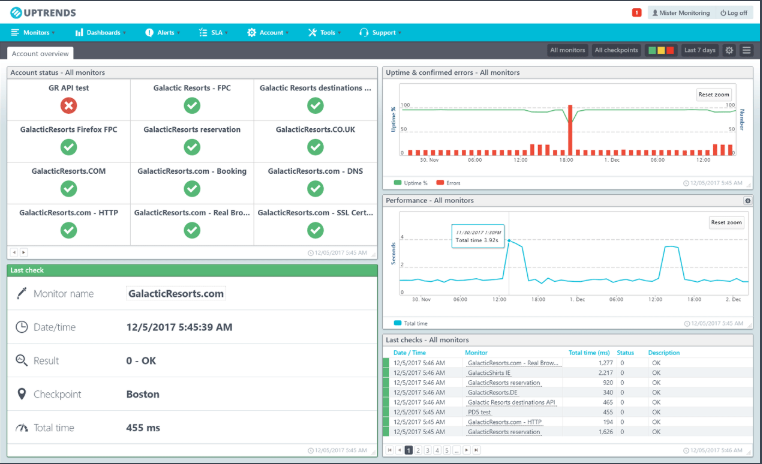
\includegraphics[width=30em]{immagini/sla/websitemonitor.png}
\caption{Schermata esemplificativa di Uptrends - Website Uptime Monitoring}
\end{figure}

Questo strumento software permette di monitorare:

\begin{itemize}
	\item le richieste HTTP/HTTPS;
    \item i webservice (SOAP, REST API);
    \item i certificati SSL;
    \item i DNS;
    \item i server.
\end{itemize}

Viene utilizzato principalmente durante le attività di valutazione dello stato attuale e di valutazione degli SLAs, OLAs ed UCs preesistenti. La velocità di installazione e la comodità d'uso sono controbilanciate dalla scarsa profondità delle informazioni ricavate, che comunque corrispondono adeguatamente alle necessità del nuovo dipartimento IT durante i primi mesi dalla firma del contratto. Per ulteriori informazioni riguardo ad Uptrends - Website Uptime Monitoring consultare la sezione \href{https://www.uptrends.com/products/website-monitoring}{Website Monitoring} presente nel sito web di Uptrends.
\\
Uptrends - Website Uptime Monitoring verrà sostituito il prima possibile (idealmente entro cinque mesi) con analoghi moduli presenti in SAP Solution Manager - IT Service Management.

\subsubsection{Uptrends - API Monitoring}

\begin{figure}[H]
\centering
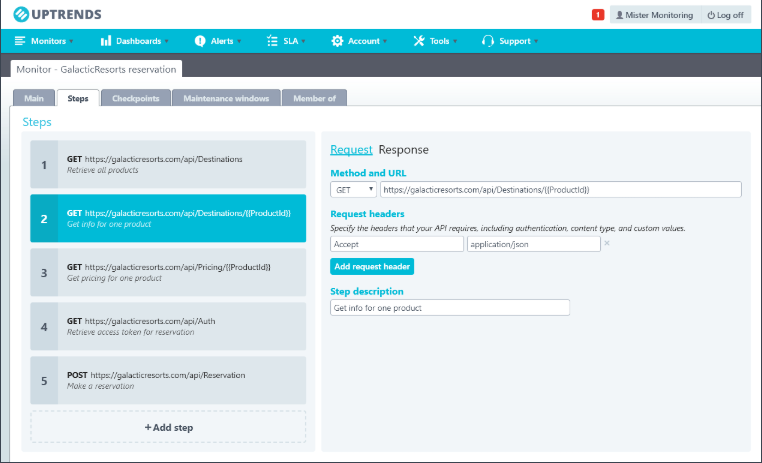
\includegraphics[width=30em]{immagini/sla/apimonitor.png}
\caption{Schermata esemplificativa di Uptrends - API Monitoring}
\end{figure}

Questo strumento software permette di monitorare:

\begin{itemize}
	\item le situazioni con chiamate API multiple;
    \item il corretto funzionamento delle API;
    \item il downtime delle API per il calcolo degli SLAs;
    \item il rispetto dei tempi massimi di risposta delle API;
    \item gli avvisi in caso di malfunzionamento delle API.
\end{itemize}

Viene utilizzato principalmente durante le attività di valutazione degli SLAs, OLAs ed UCs preesistenti e di definizione delle modalità di monitoraggio. L'installazione e la configurazione possono presentare qualche difficoltà nel caso in cui le API non siano ben strutturate e documentate, ma le informazioni ricavate sono dettagliate e facilmente personalizzabili. La possibilità di effettuare controlli continui permette una notevole tempestività da parte del nuovo dipartimento IT fin dai primi mesi dopo il suo insediamento. Per ulteriori informazioni riguardo ad Uptrends - API Monitoring consultare la sezione \href{https://www.uptrends.com/solutions/api-monitoring}{Multi-step API Monitoring} presente nel sito web di Uptrends.
\\
Uptrends - API Monitoring verrà sostituito solo all'avvento della versione finale del processo di SLA Management (idealmente entro otto mesi) con analoghi moduli presenti in SAP Solution Manager - IT Service Management.

\subsubsection{Uptrends - External Server Monitoring}

\begin{figure}[H]
\centering
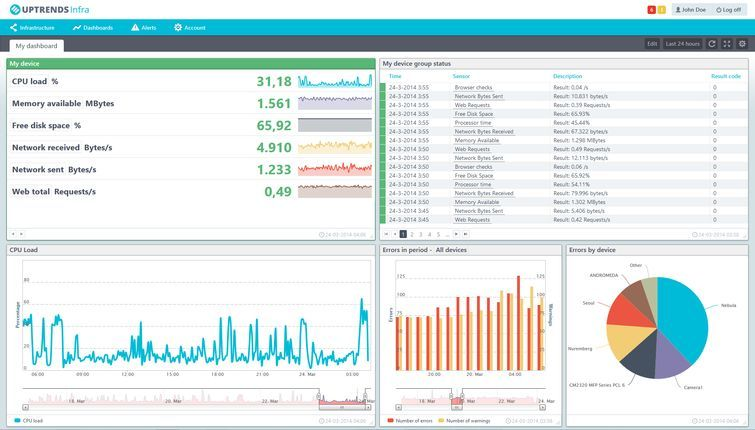
\includegraphics[width=30em]{immagini/sla/servermonitor.png}
\caption{Schermata esemplificativa di Uptrends - External Server Monitoring}
\end{figure}

Questo strumento software permette di monitorare:

\begin{itemize}
	\item i server di posta elettronica;
    \item i database SQL;
    \item i webserver.
\end{itemize}

Viene utilizzato principalmente durante le attività di valutazione dello stato attuale e di valutazione degli SLAs, OLAs ed UCs preesistenti. Gli elementi monitorati sono esclusivamente di dominio interno al nuovo dipartimento IT (dunque non riguardanti i servizi erogati da terze parti) così da garantire la stabilità dei sistemi informatici nelle situazioni di ordinaria amministrazione. Per ulteriori informazioni riguardo ad Uptrends - External Server Monitoring consultare la sezione \href{https://www.uptrends.com/products/external-server-monitoring}{External Server Monitoring} presente nel sito web di Uptrends.
\\
Uptrends - External Server Monitoring verrà sostituito durante l'implementazione del processo di SLA Management (idealmente entro sette mesi) con analoghi moduli presenti in SAP Solution Manager - IT Service Management.

\subsubsection{SAP Solution Manager - IT Service Management}

\begin{figure}[H]
\centering
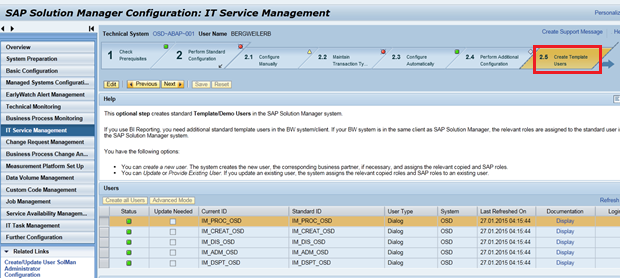
\includegraphics[width=30em]{immagini/sla/itservicemanagement.png}
\caption{Schermata esemplificativa di SAP Solution Manager - IT Service Management}
\end{figure}

Questo strumento software permette di automatizzare ogni aspetto relativo agli SLAs dei servizi erogati dal nuovo dipartimento IT. In particolare risolve i seguenti punti chiave per il nuovo processo di SLA Management:

\begin{itemize}
	\item la creazione di servizi e profili di risposta;
	\item la configurazione generica del processo di SLA Management;
	\item la definizione delle procedure per il rilevamento degli SLAs nei vari casi d'uso;
	\item la configurazione della procedure di escalation, permettendone anche l'invio di notifiche attraverso email;
	\item la definizione di specifiche caratteristiche per il monitoraggio ed il reporting degli SLAs.
\end{itemize}

In quanto la gestione degli SLAs sarà interamente automatizzata, la corretta configurazione di questo software sarà estremamente importante, nonchè lunga e delicata. Per illustrare il funzionamento di SAP Solution Manager - IT Service Management, presentiamo sinteticamente un caso d'uso esemplificativo: la gestione degli SLAs in occasione di un incidente relativo ad un configuration item fornito da un venditore di hardware.
\\ \\
Dopo aver effettuato l'accesso al proprio sistema SAP, si ha accesso alla schermata di SAP Solution Manager IT Service Management. Visualizzando l'incidente, si può verificare come il venditore di hardware ed il codice del configuration item siano stati rilevati automaticamente dal software.

\begin{figure}[H]
\centering
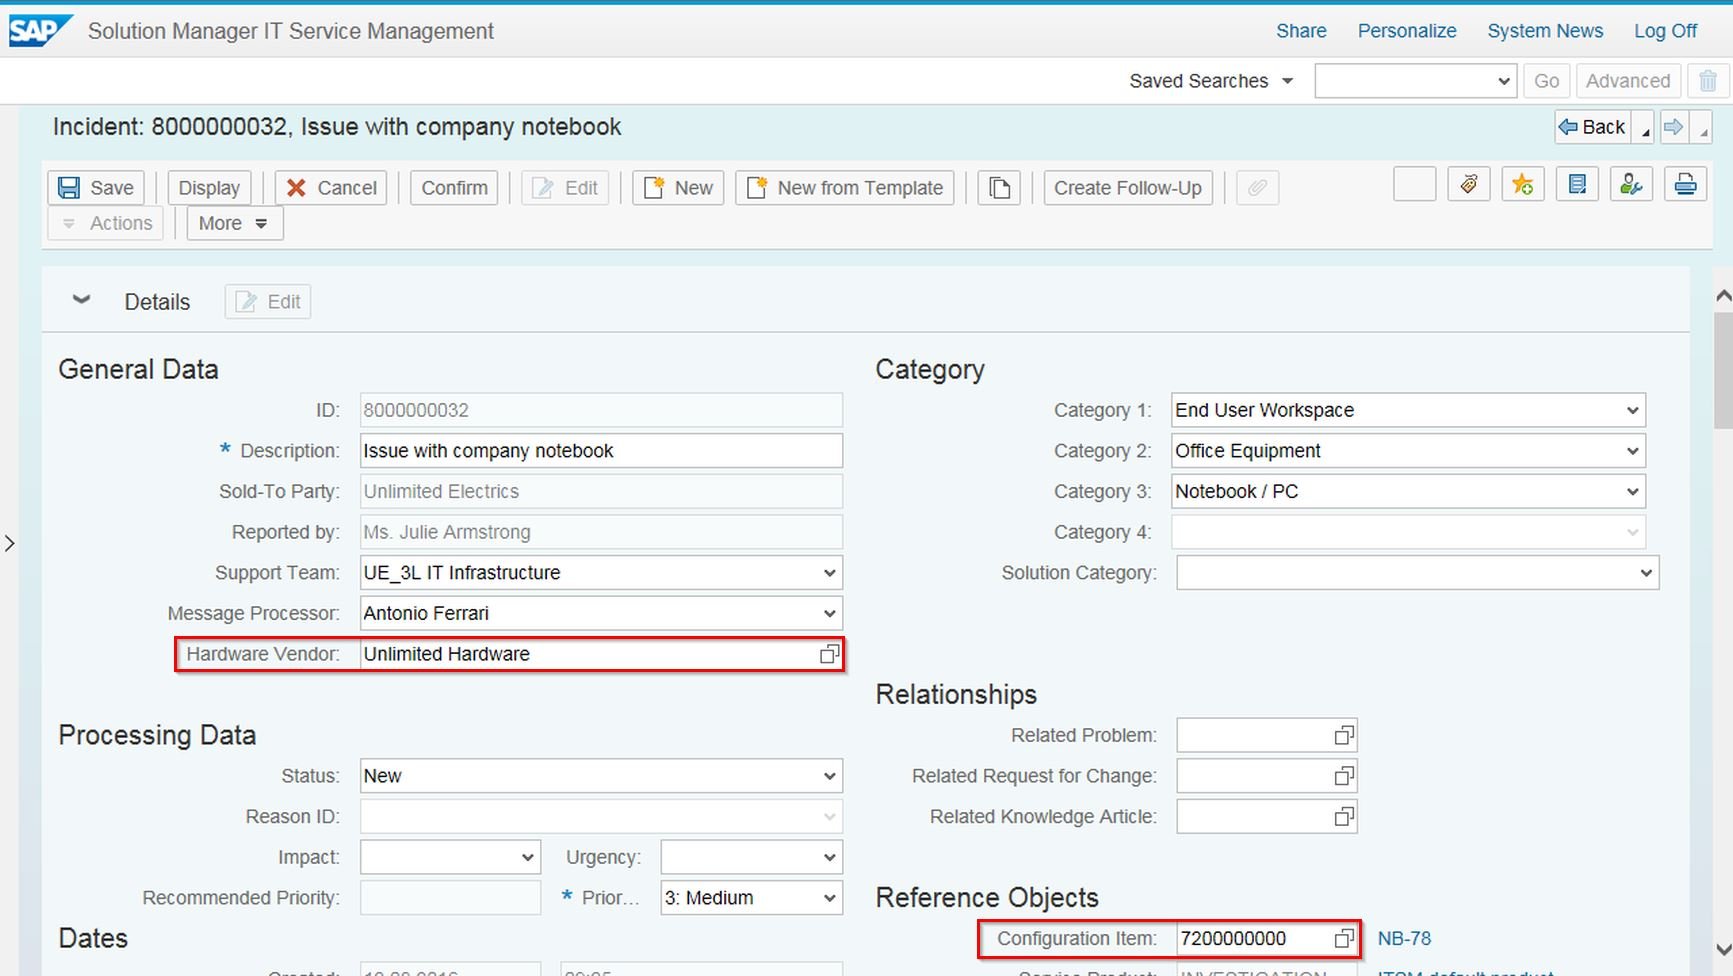
\includegraphics[width=30em]{immagini/sla/sm1.png}
\caption{Caso d'uso - Visualizzazione dell'incidente}
\end{figure}

I tempi operativi per OLAs ed UCs risultano non calcolati, infatti non è stato ancora stabilito lo status dell'incidente.

\begin{figure}[H]
\centering
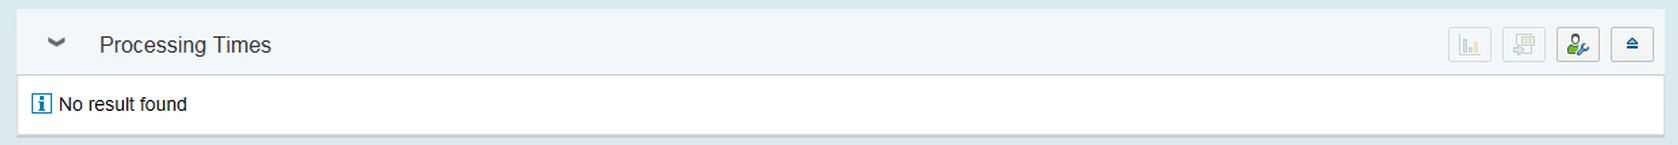
\includegraphics[width=30em]{immagini/sla/sm2.png}
\caption{Caso d'uso - Visualizzazione dei tempi di OLAs ed UCs}
\end{figure}

Appena il dipartimento IT definisce lo status dell'incidente, cioè un difetto nell'hardware, questo viene aggiornato. Il software rileva un contratto attivo con il venditore di hardware, lo notifica ed inizia il calcolo dei parametri concordati nell'UC con tale venditore.

\begin{figure}[H]
\centering
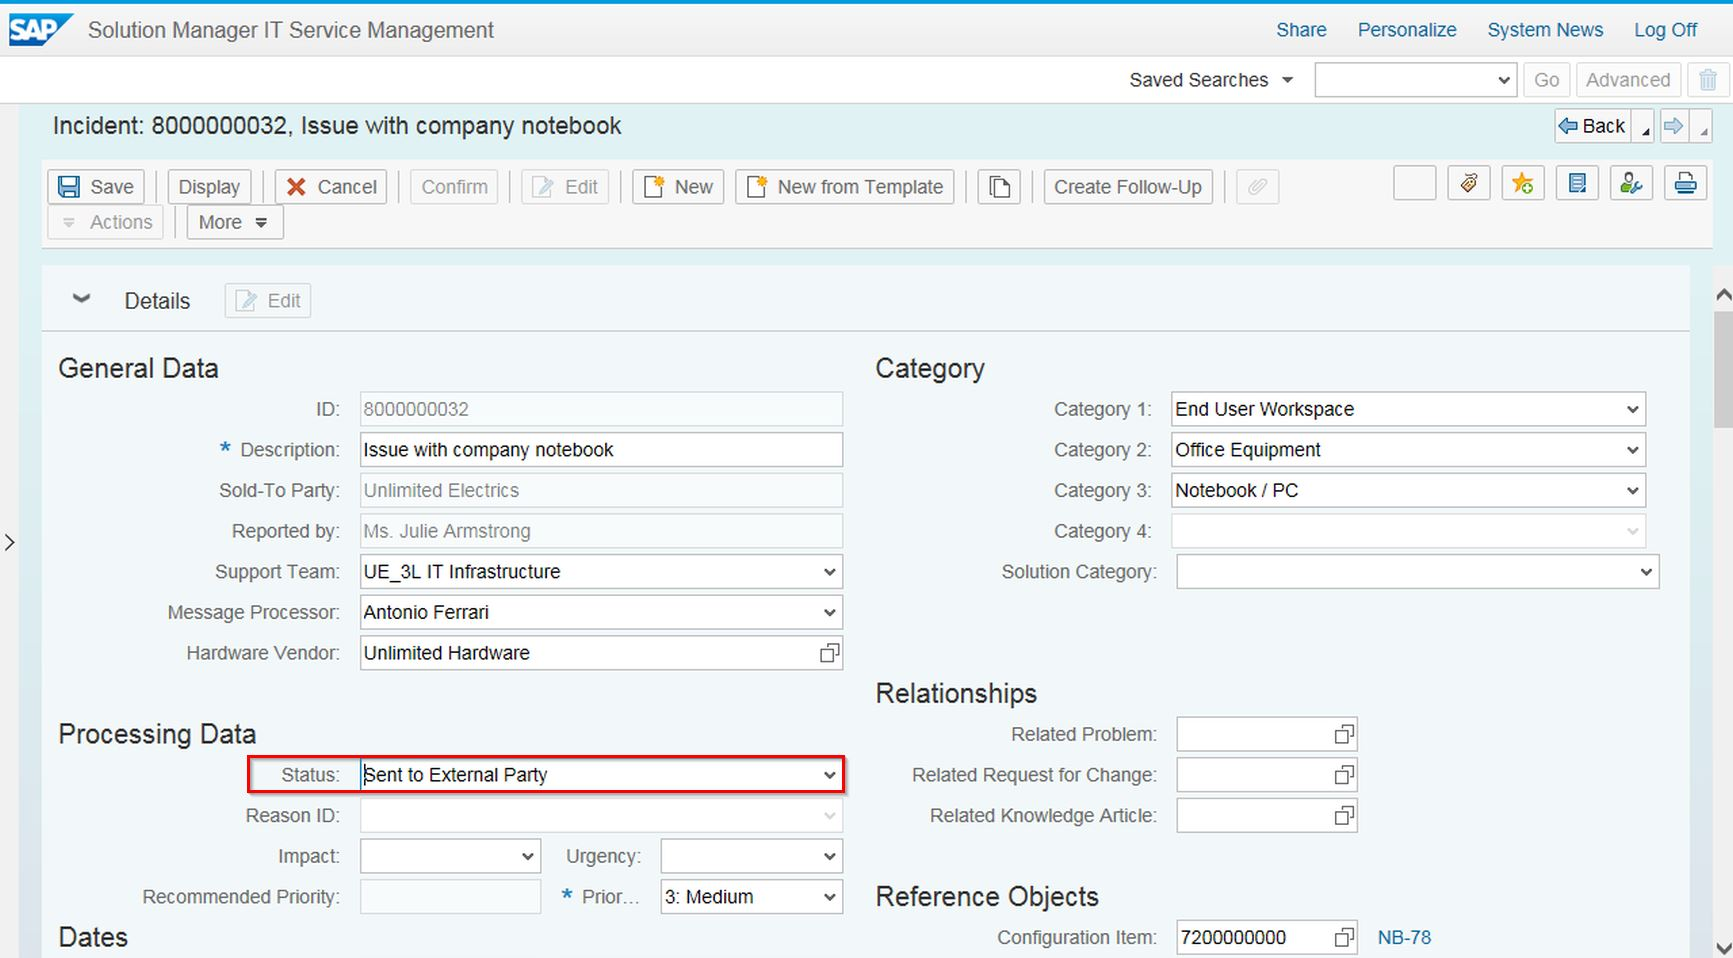
\includegraphics[width=30em]{immagini/sla/sm3.png}
\caption{Caso d'uso - Aggiornamento dello status dell'incidente}
\end{figure}

I tempi operativi per l'UC con il venditore di hardware sono inizializzati e calcolati.

\begin{figure}[H]
\centering
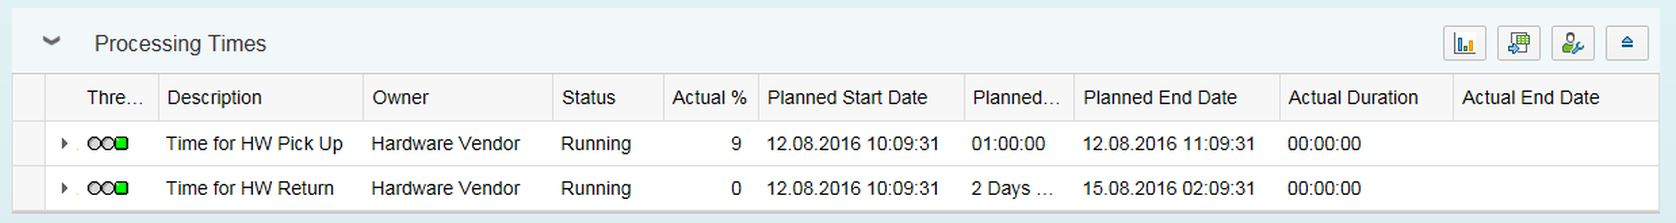
\includegraphics[width=30em]{immagini/sla/sm4.png}
\caption{Caso d'uso - Visualizzazione dei tempi di OLAs ed UCs aggiornati}
\end{figure}

Quando l'hardware viene riparato e riconsegnato, e dunque l'incidente viene chiuso, si possono visualizzare le tempistiche del venditore di hardware ed il loro rispetto delle soglie concordate nell'UC.

\begin{figure}[H]
\centering
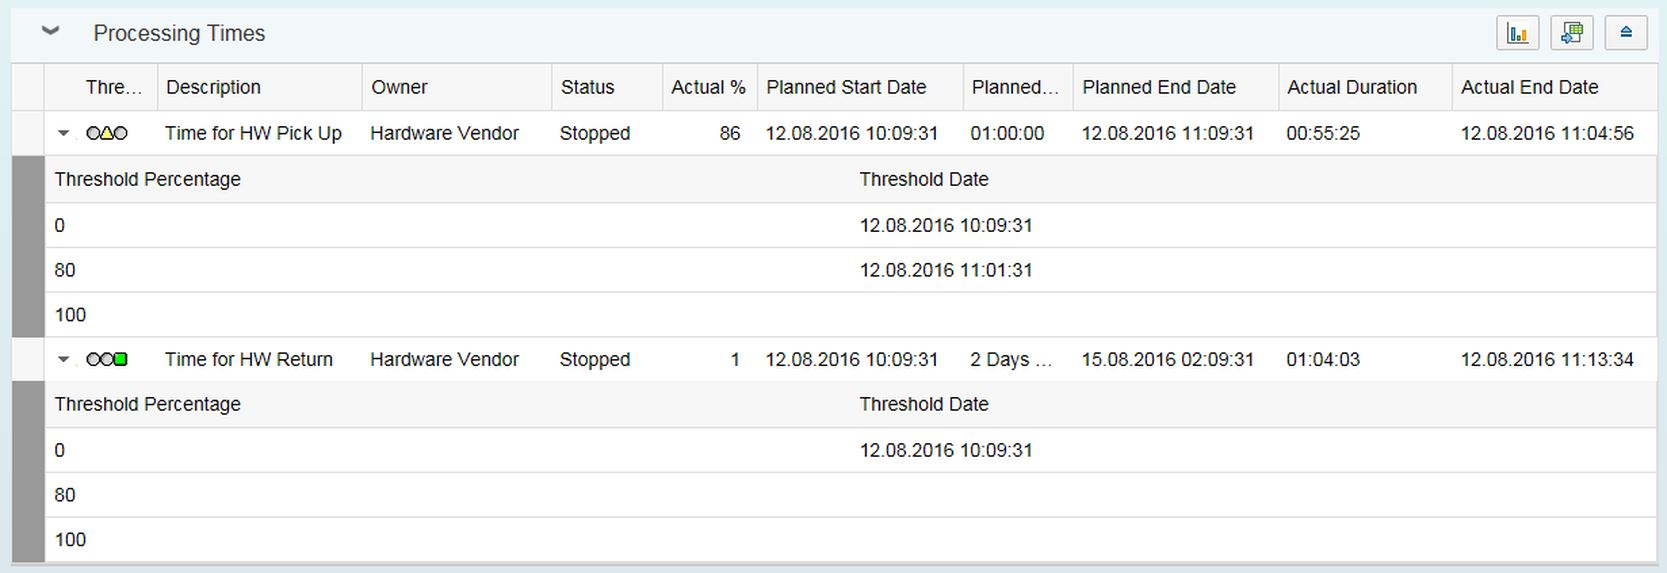
\includegraphics[width=30em]{immagini/sla/sm5.png}
\caption{Caso d'uso - Visualizzazione delle soglie temporali per l'UC}
\end{figure}

Per ogni servizio erogato all'Azienda Ospedialiera, la nostra organizzazione vuole raggiungere un simile livello di automatizzazione e dettaglio. Per ulteriori informazioni riguardo a SAP Solution Manager - IT Service Management consultare la sezione \href{https://wiki.scn.sap.com/wiki/display/SAPITSM/Service+Level+Management}{Service Level Management} presente nella community wiki di SAP Solution Manager.

\subsubsection{SAP Solution Manager - Service Desk}

\begin{figure}[H]
\centering
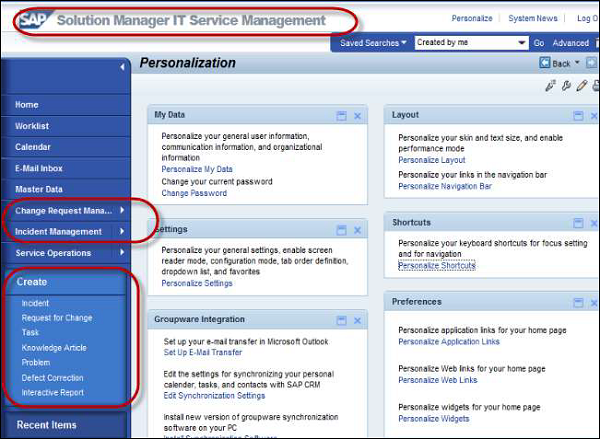
\includegraphics[width=30em]{immagini/sla/servicedesk.png}
\caption{Schermata esemplificativa di SAP Solution Manager - Service Desk}
\end{figure}

Questo strumento software permette principalmente di gestire incidenti e service requests, garantendo l'adeguato livello di supporto agli utenti. Per illustrare il funzionamento di SAP Solution Manager - Service Desk, presentiamo sinteticamente un caso d'uso esemplificativo: la creazione e la gestione di un ticket.
\\ \\
Dopo aver effettuato l'accesso al proprio sistema SAP, si ha accesso al menù SAP Easy Access. Dal menù Help > Create Support Message si può passare alla compilazione del ticket. Possono essere specificati parametri come le componenti affette, la priorità, il tipo ed i commenti.

\begin{figure}[H]
\centering
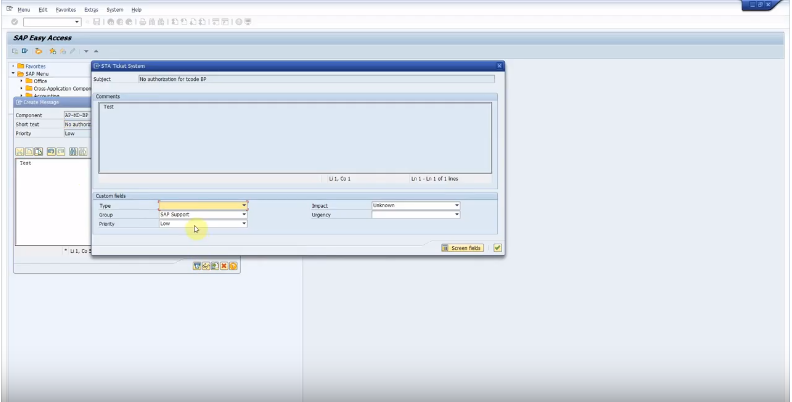
\includegraphics[width=30em]{immagini/sla/sd1.png}
\caption{Caso d'uso - Creazione del ticket}
\end{figure}

Una volta terminata la compilazione, compare un messaggio di invio con successo nel sistema di ticketing.

\begin{figure}[H]
\centering
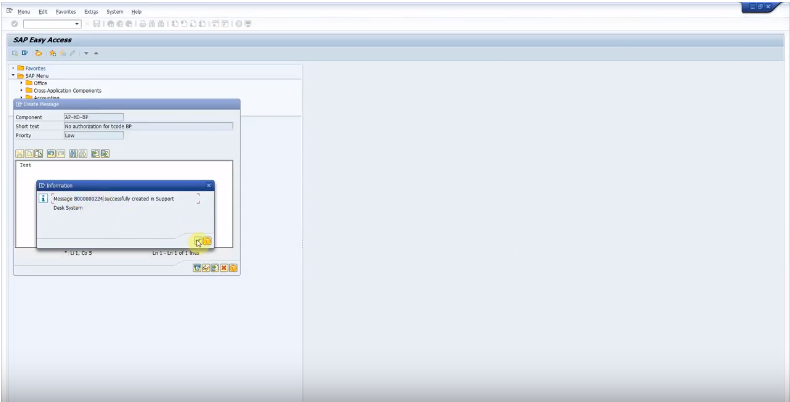
\includegraphics[width=30em]{immagini/sla/sd2.png}
\caption{Caso d'uso - Conferma ed invio del ticket}
\end{figure}

Per creare un incidente a partire dal messaggio di supporto, si deve accedere al Transaction Monitor, per poi eseguire una transazione con il codice corrispondente a quello assegnato al messaggio di supporto.

\begin{figure}[H]
\centering
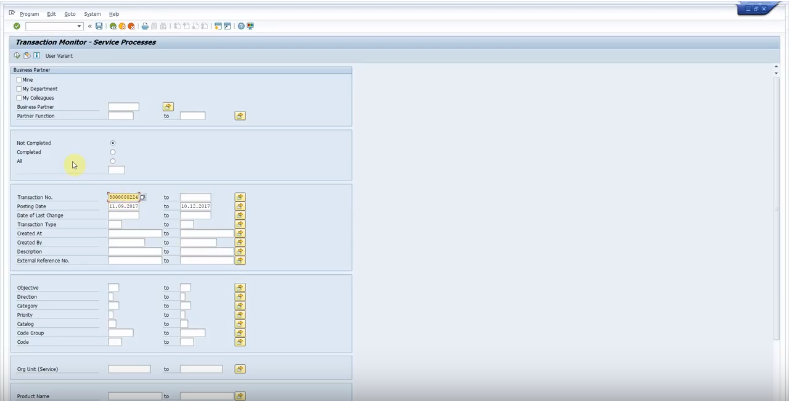
\includegraphics[width=30em]{immagini/sla/sd3.png}
\caption{Caso d'uso - Creazione dell'incidente}
\end{figure}

Il nuovo ticket sarà ora visibile nella schermata di Transaction Monitor.

\begin{figure}[H]
\centering
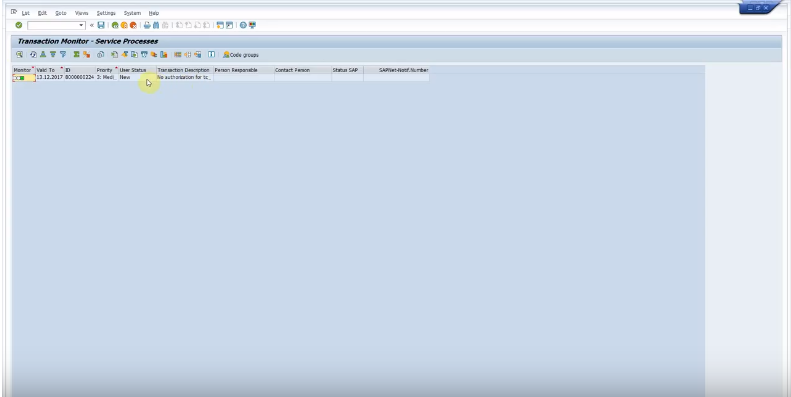
\includegraphics[width=30em]{immagini/sla/sd4.png}
\caption{Caso d'uso - Visualizzazione del ticket nella coda}
\end{figure}

Tra le varie informazioni dettagliate riguardo all'incidente, sarà disponibile automaticamente anche un report in formato pdf.

\begin{figure}[H]
\centering
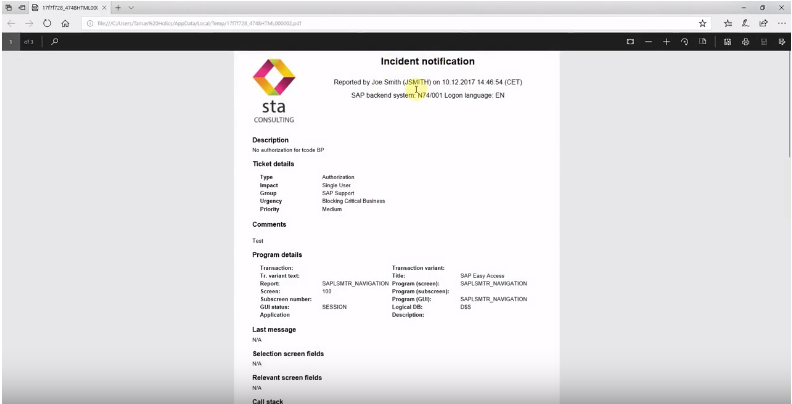
\includegraphics[width=30em]{immagini/sla/sd5.png}
\caption{Caso d'uso - Report dell'incidente}
\end{figure}

Certamente l'uso del software SAP Solution Manager - Service Desk non si riduce al semplice caso d'uso qui presentato. Per ulteriori informazioni riguardo a SAP Solution Manager - Service Desk consultare la sezione \href{https://support.sap.com/en/solution-manager/solution-manager-71/processes-71/it-service-management.html}{IT Service Management} presente in SAP Support Portal.

\subsubsection{Soluzione ad hoc - Interfaccia SLA Manager}

\begin{figure}[H]
\centering
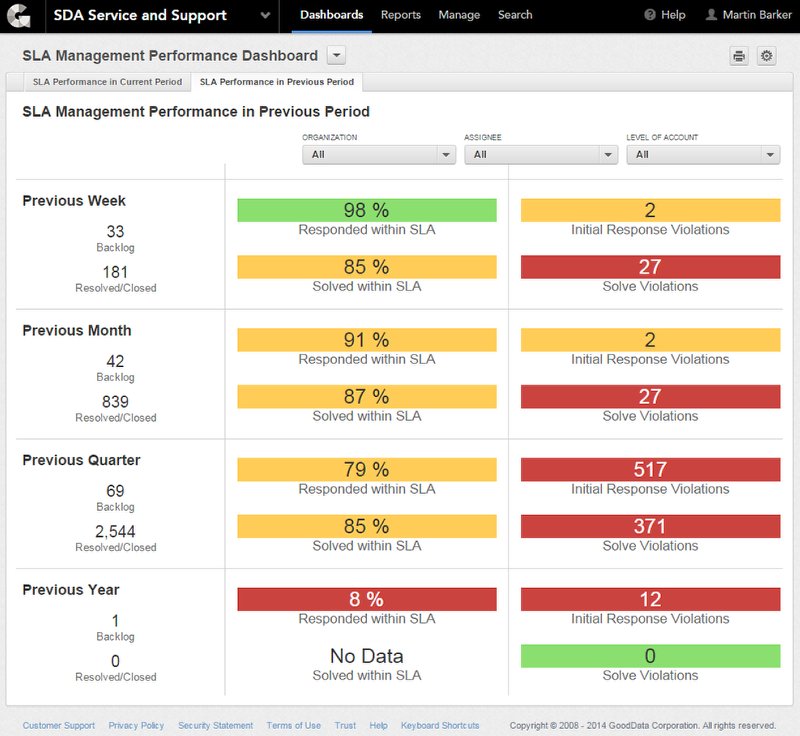
\includegraphics[width=30em]{immagini/sla/slainterface.png}
\caption{Schermata esemplificativa della soluzione ad hoc di interfaccia SLA Manager}
\end{figure}

Come definito nel Capitolato Tecnico, sezione 5.1.4.5 - Misurazione dei livelli di servizio (SLA Management), il sistema informativo dedicato alla gestione degli SLA viene denominato SLA Manager. Durante le attività di avviamento sarà disponibile una soluzione ad hoc provvisoria, consultabile attraverso un'interfaccia semplificata. Gli strumenti software di Uptrends risultano troppo tecnici per il personale non specializzato nell'ambito informatico. La nostra organizzazione ha definito un template standard per riunire tutte le informazioni rilevate dai vari strumenti ed unificarle in un'interfaccia user-friendly. Durante le attività di analisi dello stato attuale e scelta dei responsabili del processo di SLA Management, sono stati definiti specifici gruppi di utenti che potranno consultare ad esempio:

\begin{itemize}
	\item da un singolo servizio all'intero Service Catalogue;
    \item dal semplice stato online/offline alle varie metriche e KPIs monitorati;
    \item dalle informazioni in tempo reale a quelle documentati nei periodi passati.
\end{itemize}

Sebbene durante le attività di avviamento questa soluzione ad hoc sarà ancora provvisoria e probabilmente soggetta a variazioni, riteniamo sia un'ottima scelta anche successivamente all'implementazione del nuovo processo di SLA Management. In tal modo, anche quando la migrazione totale a SAP Solution Manager sarà ultimata, il personale non noterà alcun cambiamento sostanziale nell'interfaccia. Inoltre questo strumento, essendo sviluppato internamente alla nostra organizzazione, potrà adattarsi alle necessità future dell'Istituto e garantire un alto grado di flessibilità.

\subsection{Strumenti software a supporto delle attività di conduzione}

Durante le attività di conduzione, la gestione dei servizi sarà stabile e ben definita (siano essi erogati internamente al nuovo dipartimento IT oppure da fornitori di terze parti). Tutti i servizi interni saranno strettamente collegati al software SAP Solution Manager, dando così vita ad un sistema informativo centralizzato (etichettato come "SLA Manager" nel Capitolato Tecnico). Tutti i servizi esterni dovranno ugualmente essere compatibili e collegati al software SAP Solution Manager, in caso contrario dovranno essere migrati internamente al nuovo dipartimento IT. SAP Solution Manager è uno strumento software estremamente complesso e ramificato, che necessita di tempo per le operazioni di installazione, configurazione e rilascio. Grazie alla sua modularità, alcune sue funzionalità sono state già integrate con il nuovo processo di SLA Management durante le attività di avviamento. L'integrazione dei restanti moduli verrà effettuata durante le attività di conduzione in maniera graduale, in base alla pianificazione precedentemente elaborata.
\\
Segue una breve spiegazione delle funzionalità e dei moduli chiave necessari al processo di SLA Management.

\subsubsection{SAP Solution Manager - IT Service Management}

Questo strumento software sarà già stato utilizzato durante le attività di avviamento, in quanto offre un'ampia gamma di funzionalità indispensabili. I casi d'uso in cui verrà impiegato saranno gradualmente estesi, fino a coprire la quasi interezza (escludendo l'interfaccia) del nuovo sistema informativo, lo SLA Manager. Le principali funzionalità che integreremo nello SLA Manager saranno:

\begin{itemize}
	\item Incident Management, ovvero la gestione degli incidenti;
    \item Problem Management, ovvero la gestione dei problemi;
    \item Request Fulfillment, ovvero la gestione delle Service Request;
    \item Change Request, ovvero la gestione delle richiesti di modifiche ai servizi;
    \item Service Catalogue Management, ovvero la gestione dei cambiamenti apportati al Service Catalogue.
\end{itemize}

Per ulteriori informazioni riguardo a SAP Solution Manager - IT Service Management consultare la sezione \href{https://support.sap.com/en/solution-manager/solution-manager-71/processes-71/it-service-management.html}{IT Service Management} presente in SAP Support Portal, nonchè le sezioni \href{https://wiki.scn.sap.com/wiki/display/SAPITSM/IT+Service+Management+Wiki+for+User}{IT Service Management for User} e \href{https://wiki.scn.sap.com/wiki/display/SAPITSM/ITSM+Wiki+for+Administrator}{IT Service Management for Administrator} presenti nella community wiki di SAP Solution Manager.
\\
Per approfondire l'implementazione del processo di Incident Management in SAP Solution Manager consultare la sezione \href{https://wiki.scn.sap.com/wiki/display/SM/Incident+Management+Overview}{Incident Management} presente nella community wiki di SAP Solution Manager.
\\
Per approfondire l'implementazione del processo di Incident Management in SAP Solution Manager consultare la sezione \href{https://help.sap.com/viewer/0611cd2e5d1e403c9ee7b6efad89e81b/7.2.07/en-US/1f35fb5cda804e71bfcf5c00326eb1fa.html}{Problem Management} presente in SAP Help Portal.
\\
Per approfondire l'implementazione del processo di Request Fulfillment in SAP Solution Manager consultare la sezione \href{https://wiki.scn.sap.com/wiki/display/SAPITSM/Service+Request+Management+Service+Request+Fulfillment}{Service Request Fulfillment} presente nella community wiki di SAP Solution Manager.
\\
Per approfondire l'implementazione del processo di Change Request Management in SAP Solution Manager consultare la sezione \href{https://wiki.scn.sap.com/wiki/display/SM/Change+Request+Management+Overview}{Change Request Management} presente nella community wiki di SAP Solution Manager.
\\
Per approfondire l'implementazione del processo di Service Catalogue Management in SAP Solution Manager consultare la sezione \href{https://wiki.scn.sap.com/wiki/display/SAPITSM/Service+Catalogue+Management}{Service Catalogue Management} presente nella community wiki di SAP Solution Manager.

\subsubsection{SAP Solution Manager - Monitoring}

SAP Solution Manager abilita funzionalità di:

\begin{itemize}
	\item System Monitoring, cioè il monitoraggio di elementi informatici come istanze, database ed host;
    \item Connection Monitoring, cioè il monitoraggio delle connessioni presenti nel proprio sistema informatico;
    \item Business Intelligence Monitoring, cioè il monitoraggio della corretta esecuzione delle operazioni effettuate nel proprio sistema informatico e la generazione di report su di esse;
    \item Process Integration Monitoring, cioè il monitoraggio dell'integrazione tra diversi componenti del proprio sistema informatico;
    \item End-User Experience Monitoring, cioè il monitoraggio di performance ed availability del proprio sistema informatico rispetto ai vari punti di contatto disponibili.
\end{itemize}

Per ulteriori informazioni riguardo a SAP Solution Manager - System Monitoring consultare le sezioni \href{https://wiki.scn.sap.com/wiki/display/TechOps/Solution+Manager+7.2+-+System+Monitoring}{System Monitoring} e \href{https://wiki.scn.sap.com/wiki/display/TechOps/System+Monitoring+7.2+-+Advanced+Monitoring}{Advanced Monitoring} presenti nella community wiki di SAP Solution Manager.
\\
Per ulteriori informazioni riguardo a SAP Solution Manager - Connection Monitoring consultare la sezione \href{https://wiki.scn.sap.com/wiki/display/TechOps/Interface+and+Connection+Monitoring+Setup+with+SAP+Solution+Manager+7.2}{Interface and Connection Monitoring Setup} presente nella community wiki di SAP Solution Manager.
\\
Per ulteriori informazioni riguardo a SAP Solution Manager - Business Intelligence Monitoring consultare la sezione \href{https://wiki.scn.sap.com/wiki/display/SMAUTH/Technical+Monitoring+-+Business+Intelligence+Monitoring}{Business Intelligence Monitoring} presente nella community wiki di SAP Solution Manager.
\\
Per ulteriori informazioni riguardo a SAP Solution Manager - Process Integration Monitoring consultare la sezione \href{https://wiki.scn.sap.com/wiki/display/TechOps/Central+PI+Monitoring+with+SAP+Solution+Manager+7.2}{Process Integration Monitoring} presente nella community wiki di SAP Solution Manager.
\\
Per ulteriori informazioni riguardo a SAP Solution Manager - End-User Experience Monitoring consultare la sezione \href{https://wiki.scn.sap.com/wiki/display/EEM/Home}{End-User Experience Monitoring} presente nella community wiki di SAP Solution Manager.

\subsubsection{SAP Solution Manager - Service Level Reporting}

Questo strumento software consiste in una libreria in grado di ottimizzare e semplificare la gestione a lungo termine del monitoraggio rispetto agli SLAs del proprio sistema informatico. Basato sul monitoraggio proattivo di  SAP EarlyWatch Alert, controlla periodicamente il rispetto degli SLAs rispetto alle metriche ed ai KPIs impostati. Inoltre genera autonomamente report personalizzabili secondo le proprie necessità, notificando eventuali responsabili.
Per ulteriori informazioni riguardo a SAP Solution Manager - Service level Reporting consultare la sezione \href{https://help.sap.com/doc/saphelp_sm71_sp08/7.1.08/en-US/36/5ec6267ba34de08c55e3c310ebdece/content.htm?no_cache=true}{Service Level Reporting} presente nella documentazione delle librerie di SAP Solution Manager.
\\
Per ulteriori informazioni riguardo a SAP EarlyWatch Alert consultare la sezione \href{https://support.sap.com/en/offerings-programs/support-services/earlywatch-alert.html}{SAP EarlyWatch Alert} presente in SAP Support Portal.

\subsubsection{Soluzione ad hoc - Interfaccia SLA Manager}

\begin{figure}[H]
\centering
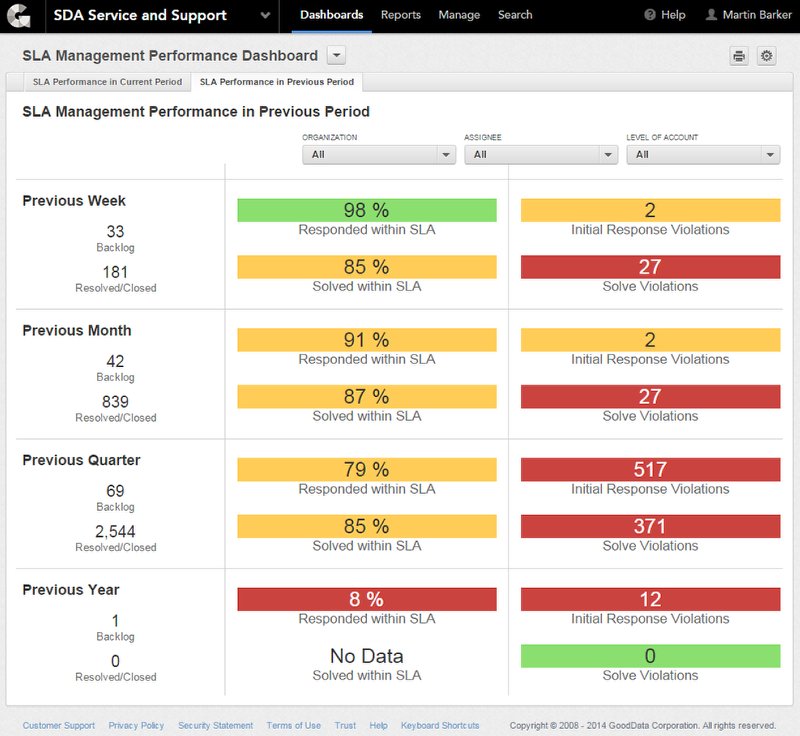
\includegraphics[width=30em]{immagini/sla/slainterface.png}
\caption{Schermata esemplificativa della soluzione ad hoc di interfaccia SLA Manager}
\end{figure}

Questo strumento software sarà già stato utilizzato durante le attività di avviamento e resterà l'interfaccia di riferimenti per il personale dell'Istituto. Verrà rilasciata una versione definitiva e stabile, che la nostra organizzazione si occuperà di mantenere ed evolvere nel tempo, secondo le necessità del business.

%**********************************************************

\section{Sistema informativo del processo di SLA Management}

La base per il sistema informativo del processo di SLA Management è costituita dal software SAP Solution Manager. Le aree cui si dedica sono:

\begin{itemize}
	\item Application Operations;
    \item Business Process Operations;
    \item Data Volume Management;
    \item Change Control Management;
    \item Custom Code Management;
    \item IT Service Management;
    \item Landscape Management;
    \item Process Management;
    \item Project Management;
    \item Test Suite;
    \item Cross Topics;
    \item Focused Solutions.
\end{itemize}

In particolare, esaudisce le richieste riguardo al nuovo processo di SLA Management presentate nel Capitolato Tecnico:

\begin{itemize}
	\item monitoraggio di SLAs, OLAs ed UCs;
    \item consultazione dello stato effettivo del sistema in tempo reale;
    \item documentazione di metriche e KPIs rilevati;
    \item scambio di informazioni tra differenti servizi, dipartimenti ed unità di business;
    \item personalizzazione in base alle specifiche caratteristiche dell'Azienda Ospedaliera;
    \item integrazione con l'ambiente di test per i servizi di sperimentazioni ed innovazioni.
\end{itemize}

Considerando tuttavia la relativa complessità di tale strumento, proponiamo il mantenimento di una soluzione ad hoc per l'interfaccia del sistema informativo denominato SLA Manager. Così facendo, manterremo la qualità di SAP Solution Manager unita alla semplicità di un'interfaccia che interpreti automaticamente le informazioni monitorate. Status, performance, metriche e KPIs dei vari servizi saranno prontamente visibili, aggiornate e soprattutto facilmente comprensibili. Il lato più tecnico sarà comunque disponibile al nuovo dipartimento IT, così da poter lavorare con il massimo dei dati e poter fornire rilevamenti più specifici se necessario.

%**********************************************************

\section{Template documenti}

Di seguito sono riportati dei documenti esemplificativi per:

\begin{itemize}
	\item Service Level Agreements;
    \item Operational Level Agreements;
    \item Underpinning Contracts.
\end{itemize}


\includepdf[pages=-]{immagini/sla/sla.pdf}

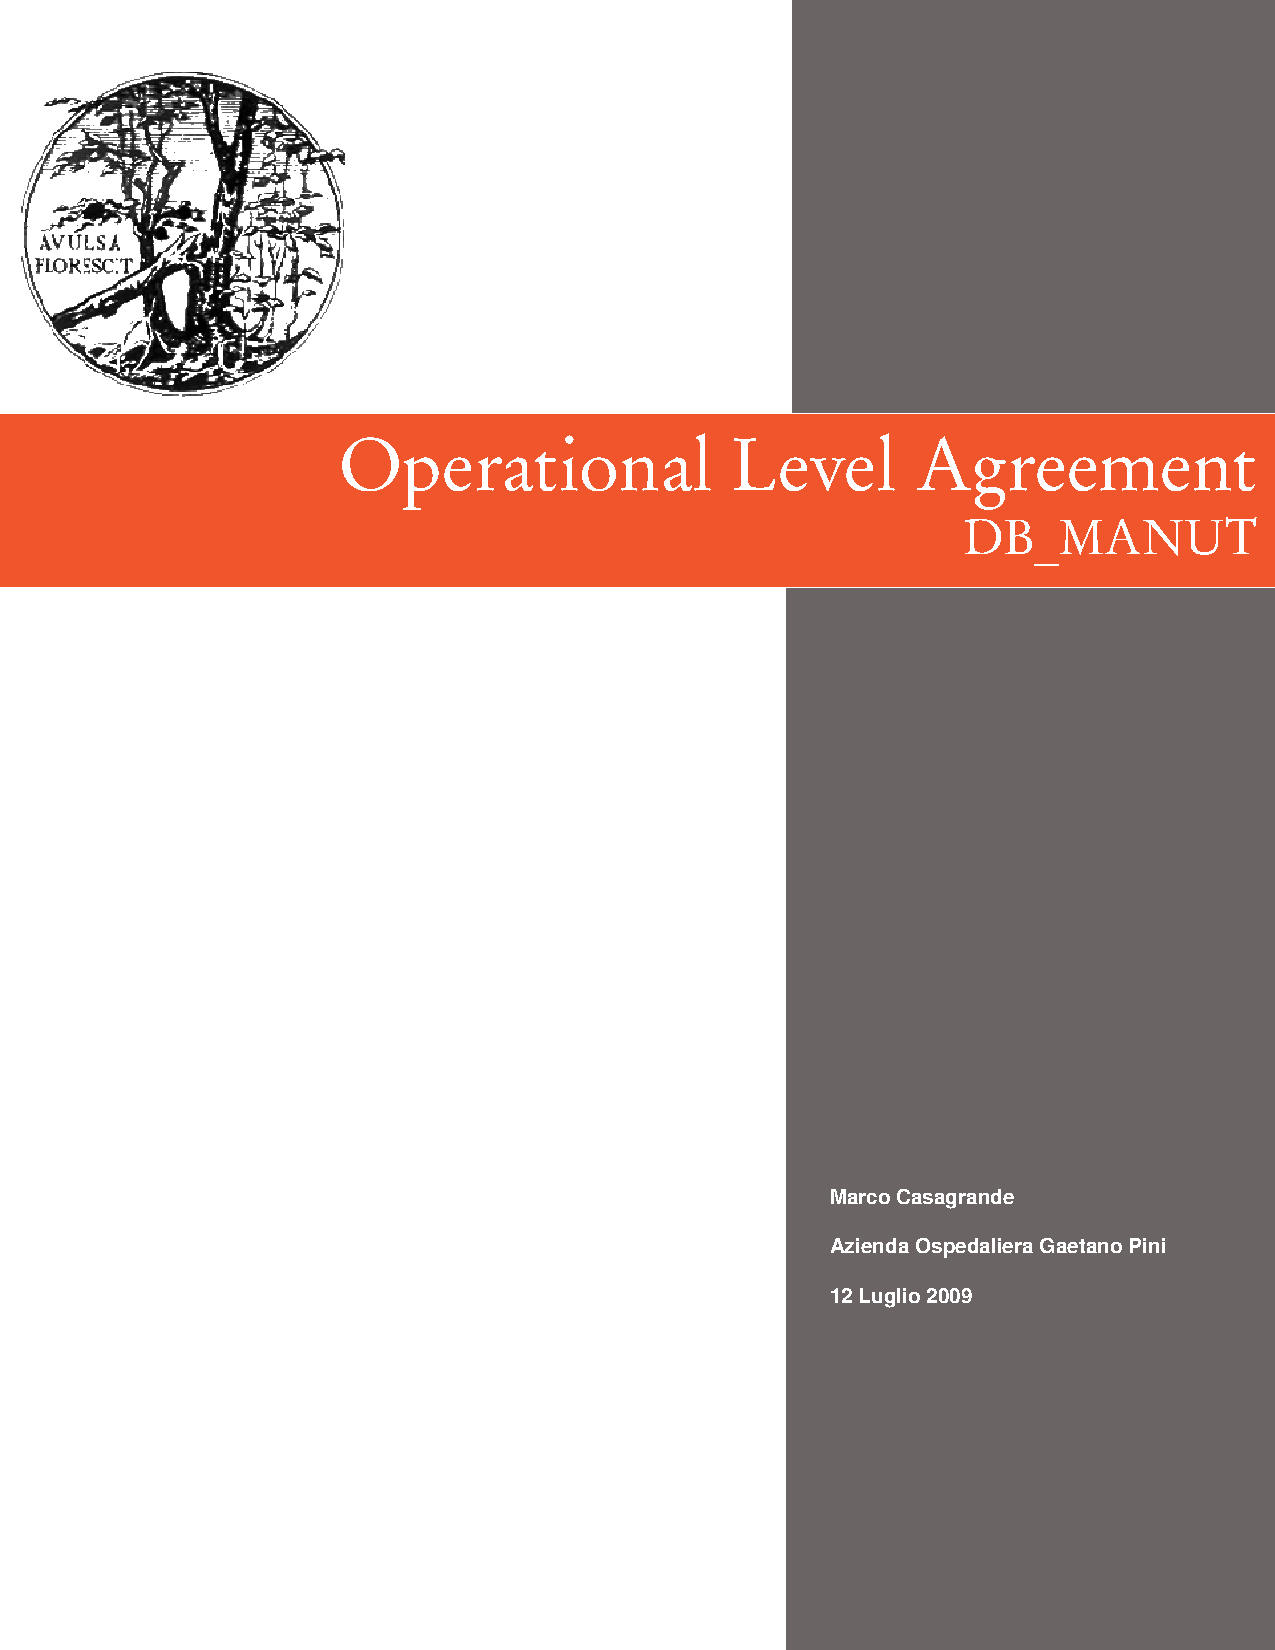
\includepdf[pages=-]{immagini/sla/ola.pdf}

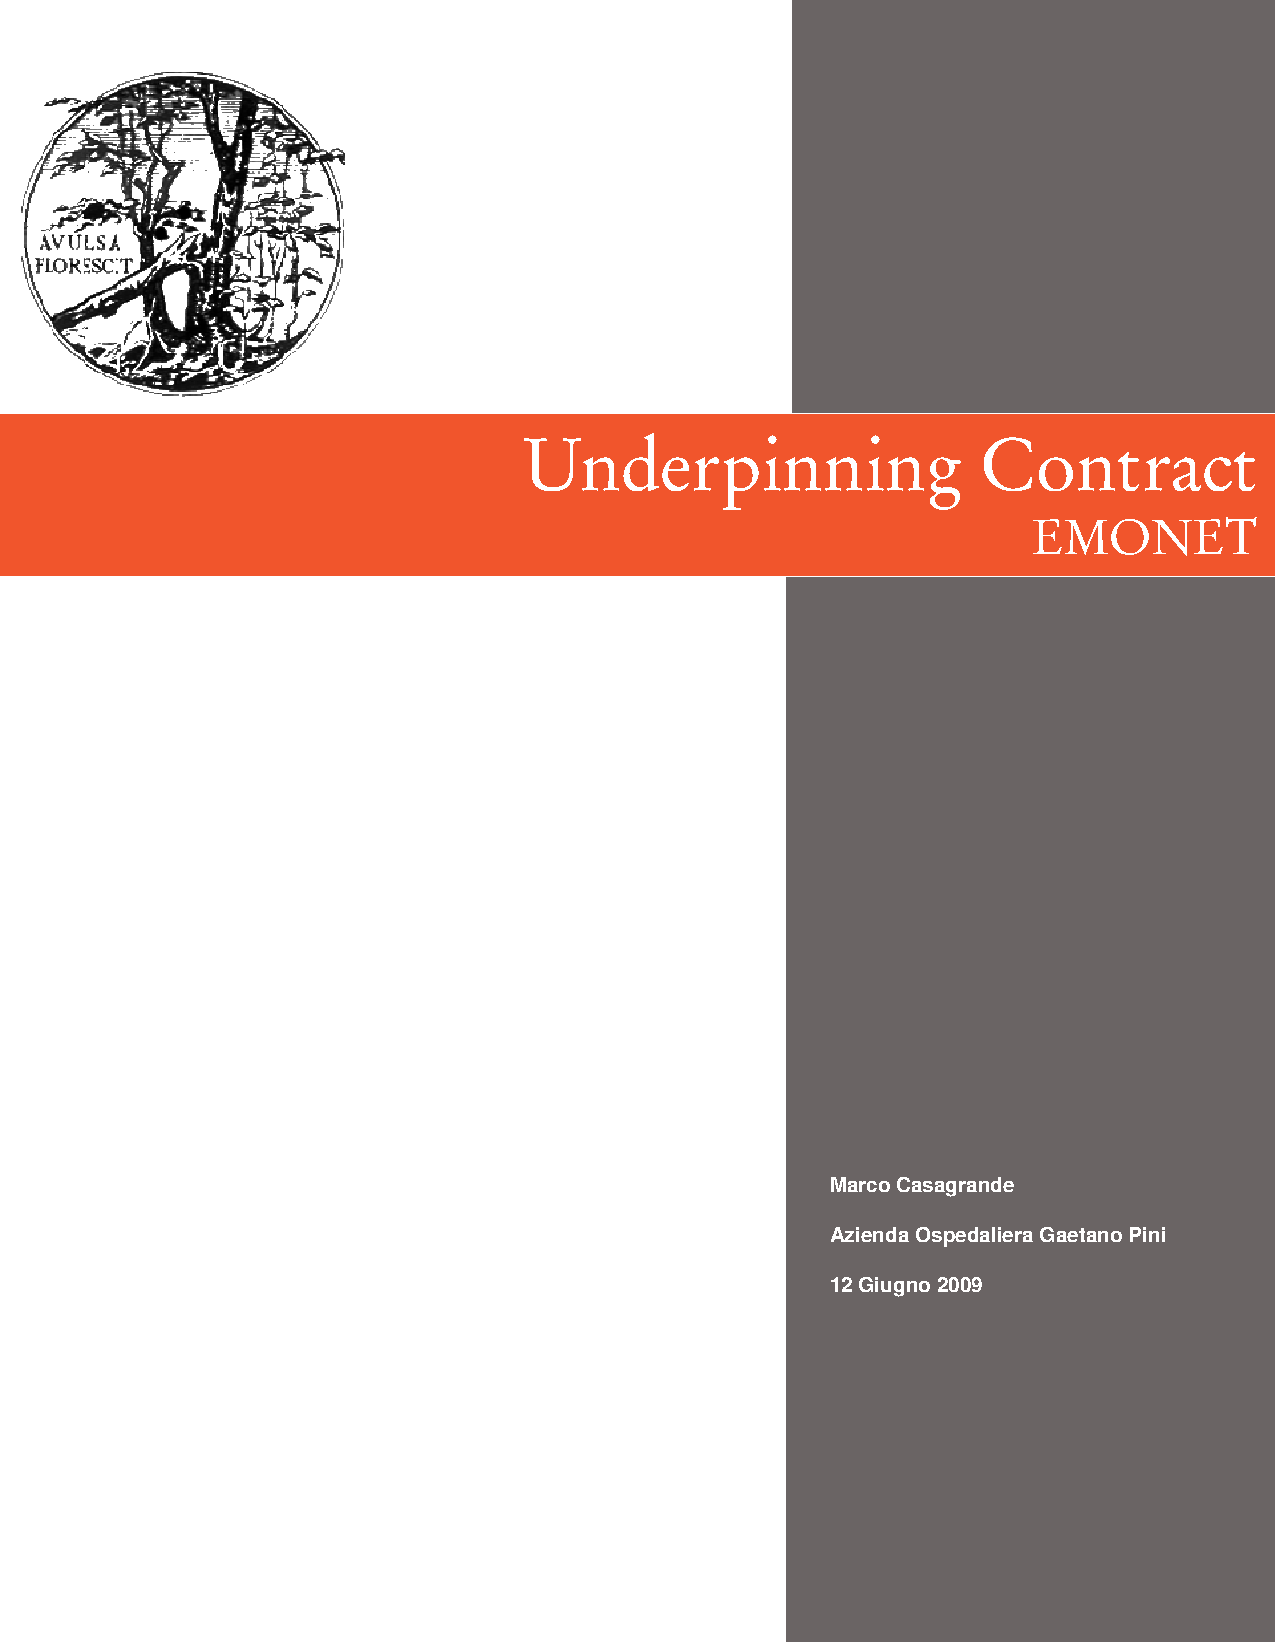
\includepdf[pages=-]{immagini/sla/uc.pdf}
             
% !TEX encoding = UTF-8
% !TEX TS-program = pdflatex
% !TEX root = ../tesi.tex
% !TEX spellcheck = it-IT

%*********************************************************
\chapter{Rollout Plan}
\begin{flushright}
\textit{a cura di \large{Jordan Gottardo}}
\end{flushright}
\label{cap:rolloutplan}


%**************************** SEZIONE 1: PANORAMICA GENERALE *******************
%*
%*
%*
	\section{Panoramica generale}
    	\subsection{Consegna}
        	\textit{L’offerente dovrà presentare un piano completo di migrazione all’attuale situazione (con differenti gestori per differenti sistemi e servizi) a quella proposta dal nuovo, unico, gestore. Il progetto dovrà includere la presa in carico dei sistemi attuali, fino alla loro eventuale sostituzione, e tutte le attività di messa in opera ed avvio dei nuovi sistemi. Dovranno essere chiaramente indicate le milestone progettuali ed in particolare i collaudi che segnano l’avvio in esercizio dei sistemi e dei servizi. Dovranno inoltre essere descritte esaurientemente tutte le attività professionali ed i task necessari sia per l’avvio e la messa a regime sia per il controllo del progetto.}
            

			Il proponente, l'Azienda Ospedaliera Gaetano Pini, richiede la stesura di un piano di migrazione (rollout) per la pianificazione delle attività atte alla messa in opera della soluzione proposta.
            
		\subsection{Rollout all'interno di ITIL}
        	Il rollout trova la sua naturale collocazione all'interno del processo di Release and Deployment Management di ITIL V3, facente parte dell'area di Service Transition. 
            
            
            Lo scopo principale di questo processo è pianificare e controllare il movimento delle release negli ambienti di test e live, assicurando che l'integrità dell'ambiente live sia protetta e che le componenti corrette siano rilasciate.
            
            \begin{figure}[H]
				\centering
				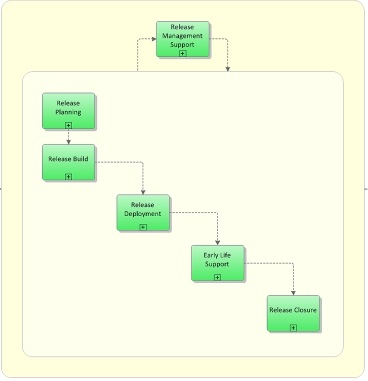
\includegraphics[scale=0.5]{immagini/rollout/release-deployment}
				\caption{Sottoprocessi di Release and Deployment Management (\url{https://goo.gl/7jCkZH}).}
			\end{figure}
         
            
            Il processo è suddiviso nei seguenti sotto-processi:
            \begin{itemize}
            	\item \textbf{Release Management Support:} fornisce linee guida e supporto per lo sviluppo delle release.
                \item \textbf{Release Planning:} assegna le change, dopo che sono state autorizzate, ai release packages e definisce la portata e i contenuti delle release. Inoltre, sviluppa uno schedule per build, test e deployment della release.
                \item \textbf{Release Build:} emette tutti gli ordini di lavoro e le richieste di acquisto per lo sviluppo interno o l'acquisizione delle componenti della release, in modo da renderli disponibili per la fase di test.
                \item \textbf{Release Deployment:} effettua il deploy delle componenti della release nell'ambiente live. Inoltre, forma gli utenti e il personale operativo e si occupa di rilasciare informazioni e documentazione sulle release di cui è stato fatto il deploy.
                \item \textbf{Early Life Support:} risolve problemi operativi nel periodo immediatamente successivo al rilascio, in cui è più probabile che essi si manifestino. Ricordiamo che durante l'Early Life Support il Service Transition affianca il Service Operations.
                \item \textbf{Release Closure:} si occupa della chiusura formale di una release dopo essersi assicurati che i log e il CMDB siano stati aggiornati.
            \end{itemize}

			È molto importante notare come in ITIL V3, rispetto alla versione precedente, siano state create interfacce aggiuntive tra i processi di \textbf{Release Management} e \textbf{Project Management (Transition Planning and Support)}, in modo da assicurarsi che i due processi siano allineati per quanto riguarda l'allocazione di risorse e la pianificazione di attività.
            
            
            La stesura del piano di rollout terrà in considerazione quanto appena esposto: non si limiterà ad essere una semplice pianificazione di attività su calendario, ma verranno descritte, nei limiti del possibile, le attività, suddividendole in compiti (tasks), e le risorse necessarie per portarle a termine con successo.
            
            \subsection{Assunzioni}
            	Data la natura di progetto universitario del documento, nel seguito del documento verrà considerata la seguente assunzione:
                \begin{itemize}
                	\item Una precisa e puntuale quantificazione delle risorse necessarie alla fornitura del servizio, tenendo conto anche gli obiettivi di crescita a medio e lungo termine, dovrebbe essere eseguita dal processo di Capacity Management, che non viene istanziato nel presente documento, tenendo conto anche di analisi più approfondite dell'ambiente del Proponente. In ogni caso, l'Offerente cercherà di effettuare delle stime iniziali di risorse. 
                \end{itemize}
                
                
		\subsection{Riferimenti}
        	Il piano di rollout prenderà spunto dal seguente template, che guida la stesura di un Project Implementation Plan:
            \begin{itemize}
            	\item \texttt{Project Implementation Plan template: \url{https://goo.gl/LSGktb}}. 
            \end{itemize}
            
            Inoltre, il piano verrà integrato seguendo altri template e verranno presi spunti e informazioni da altre fonti. Tutti questi riferimenti sono indicati di seguito:
       		\begin{itemize} 
            	\item \texttt{Rollout Plan, Frank Bergmann: \url{http://project-open.sourceforge.net/whitepapers/Project-Open-Rollout-Plan.pdf}}.
                \item \texttt{Mifos - Pilot and Rollout Plan, Grameen Foundation: \url{https://goo.gl/TcjL4s}}.
                \item \texttt{Project Charter for MoHSS HRIMS Rollout Project : \url{https://www.ihris.org/toolkit-new/scale-up/example-rollout-plan/}}.
				\item \texttt{Processo di Release and Deployment Management del framework ITIL V3: \url{https://wiki.en.it-processmaps.com/index.php/Release_and_Deployment_Management}}.
                \item \texttt{Big bang ERP implementation vs phased approach, pros and cons: \url{https://goo.gl/7M7JmS}}.
                \item \texttt{Regolamento sulla privacy 2018: \url{https://www.laleggepertutti.it/227787_privacy-cosa-cambia-a-maggio-2018}}.
                \item \texttt{Privacy by default e by design: \url{https://protezionedatipersonali.it/privacy-by-design-e-by-default}}.
                \item \texttt{Security and Privacy: an introduction to ISO 27000: \url{https://iapp.org/media/presentations/14Symposium/CS14_Introduction\%20to\%20ISO.pdf}}.
                \item \texttt{A Qualitative Risk Analysis and Management Tool: CRAMM: \url{https://goo.gl/uZzqv9}}.
                
                \item \texttt{A Processo di Service Validation and Testing del framework ITIL V3: \url{https://wiki.en.it-processmaps.com/index.php/Service_Validation_and_Testing}}.
			\end{itemize}
            
		\newpage
%**************************** SEZIONE 2: PANORAMICA GENERALE *******************
%*
%*
%*
	\section{Panoramica di gestione}
    	In questa sezione verranno descritte le dinamiche di gestione per l'implementazione della soluzione, identificando le attività principali e suddividendole in compiti (tasks).
		
        \subsection{Descrizione dell'implementazione}
			L'implementazione della soluzione seguirà le seguenti fasi:
            \begin{itemize}
            	\item \textbf{Definizione:} in questa fase verranno:
                \begin{itemize} 
                	\item Identificati, discussi e approvati i moduli che dovranno essere implementati.
                    \item Identificate le eventuali necessità di estensione.
                    \item Specificate le necessità di configurazione e personalizzazione.
                    \item Identificati i requisiti della soluzione.
                \end{itemize}
                \item \textbf{Estensione:} questa fase concerne:
                \begin{itemize}
                	\item La realizzazione di mockup iniziali per i sistemi e le applicazioni da realizzare.
                    \item La definizione di come le eventuali estensioni richieste andranno ad impattare i moduli esistenti.
                    \item L'implementazione delle estensioni richieste.
                    \item La realizzazione e la presentazione al Proponente di un prototipo.
                    \item Il completamento del prototipo e il test nell'ambiente del Proponente.
                    \item La realizzazione di documentazione tecnica e di materiale per gli utenti (manuali, ecc).
                \end{itemize}
                \item \textbf{Installazione:} durante questa fase verranno:
                \begin{itemize}
                	\item Installate le soluzioni su ambienti di produzione, di sviluppo e di test.
                    \item Configurate le soluzioni in base alle necessità di configurazione e personalizzazione definite precedentemente.
                    \item Impostati i profili utenti e assegnati i privilegi correttamente.
                    \item Importati i dati necessari al funzionamento della soluzione.
                \end{itemize}
                \item \textbf{Formazione:} in questa fase l'Offerente affiancherà il Proponente, fornendo formazione agli utenti in modo da renderli in grado di utilizzare correttamente la soluzione.
                \item \textbf{Go-live:} questa fase prevede:
                \begin{itemize}
                	\item  L'ottenimento dell'autorizzazione di entrambi Proponente e Offerente per andare live.
                    \item Trasferimento finale dei dati dal vecchio sistema a quello nuovo.
                \end{itemize}
                \item \textbf{Affiancamento:} durante il primo periodo questa fase l'Offerente affianca il Proponente, fornendo parte del team che ha lavorato all'implementazione della soluzione per risolvere dubbi, perfezionare la formazione e aiutare nell'identificazione e risoluzione di incidenti e problemi. Successivamente, si passa al periodo di supporto solamente tramite service desk.
            \end{itemize}
            

            La tipologia di rollout che verrà impiegata è di tipo \textbf{orizzontale/big bang}. Il rollout orizzontale consiste nel far adottare il nuovo sistema a tutta l'azienda nello stesso momento ("go-live"). L'alternativa a questa tipologia è il rollout verticale/phased, che prevede un rollout graduale del sistema, suddividendolo per modulo, business unit o area geografica.


            I vantaggi dell'approccio orizzontale sono:
            \begin{itemize}
            \item Tempo di implementazione più breve.
            \item Non ci sono mai due sistemi diversi utilizzati in contemporanea all'interno dell'azienda.
            \item Possibilità di creare hype in attesa del rilascio del nuovo sistema.
            \item Possibilità di concentrare la formazione esclusivamente sul nuovo sistema.
            \item Minori costi complessivi, dato che il vecchio sistema viene dismesso più in fretta.
            \end{itemize}
            Tuttavia, sono presenti anche alcuni svantaggi:
            \begin{itemize}
            \item I test di sistema sono difficili da eseguire prima del go-live.
            \item Nessuna possibilità di fall-back affidabile nel lungo periodo (dopo la dismissione del vecchio sistema).
            \item Cambiamento improvviso di abitudini di lavoro.
            \item Diminuzione temporanea di produttività.
            \end{itemize}
            Per quanto riguarda il rollout verticale, i vantaggi sono:
            \begin{itemize}
            \item Maggior facilità e minor tempo di adattamento al nuovo sistema.
            \item Possibilità di scoprire i problemi prima e risolverli in modo graduale.
            \item Maggior tempo per poter fare formazione.
            \end{itemize}
            Invece, gli svantaggi sono:
            \begin{itemize}
            \item Costi di implementazione più alti, a causa della coesistenza parziale di due sistemi diversi e dalla necessità di creazione di interfacce per favorire l'intercomunicazione.
            \item Possibilità di invalidare la conformità del sistema complessivo, a causa di incoerenze tra i due sistemi.
            \item Difficoltà di integrazione.
            \end{itemize}
            Alla luce di quanto esposto, nonostante l'approccio generale sarà di tipo orizzontale, l'Offerente ritiene di poter sfruttare un approccio verticale durante la fase di testing. Infatti sarà possibile far testare il sistema applicativo alle singole aree (Sanitaria, Amministrativa, Direzionale, Servizi) un'area alla volta, per poter effettuare formazione preventiva e identificare e risolvere in fretta eventuali problemi.
           
           
		\subsection{Punti di contatto}
        In questa sezione è possibile trovare i contatti dei membri principali del team dell'Offerente che si occuperà dell'implementazione della soluzione.
        \begin{table}[H]
        	%\renewcommand\arraystretch{1,5}
            \begin{tabular}{ c c c }
            \toprule
            \textbf{Ruolo} & \textbf{Nome} &\textbf{Numero di telefono} \\
            \toprule
            Capo progetto & Nome Cognome & 333 666444 \\
            Responsabile privacy & Nome Cognome & 333 666444 \\
            Responsabile qualità & Nome Cognome & 333 666444 \\
            Amministratore database & Nome Cognome & 333 666444 \\
            Responsabile analisi & Nome Cognome & 333 666444 \\
            Responsabile progettazione & Nome Cognome & 333 666444 \\
            \bottomrule
            \end{tabular}
            \caption{Punti di contatto}
        \end{table}

		\subsection{Attività principali}
        \label{sec:attivita}
        	In questa sezione verranno descritte le attività principali necessarie alla corretta implementazione della soluzione. Per ogni attività verranno indicate le seguenti informazioni:
            \begin{itemize}
            	\item \textbf{Deliverables:} oggetti materiali o immateriali risultanti dall'esecuzione dell'attività.
                \item \textbf{Risorse:} le risorse necessarie per l'esecuzione dell'attività.
                \item \textbf{Responsabili:} le persone (inteso come ruoli) chiave responsabili dell'attività.
                \item \textbf{Criteri di accettazione:} criteri per considerare un'attività conclusa con successo.
            \end{itemize}
            Inoltre, quando ritenuto necessario, l'attività verrà suddivisa in compiti (tasks) aventi maggiore granularità. Verranno inoltre utilizzati diagrammi di attività del linguaggio di modellazione UML3 per descrivere con maggiore precisione il flusso di esecuzione.
            
            \subsubsection{Subentro contrattuale}
            	Il Proponente desidera passare da una fornitura con service provider multipli ad una fornitura di tipo \textit{sole provider}. L'Offerente deve quindi prendere in carico la gestione di tutti i contratti esistenti alla data di aggiudicazione dell'appalto. L'Offerente reputa fondamentale avvisare i fornitori del Proponente di questa presa in carico. Nel caso in cui il fornitore non dovesse dare il benestare, l'Offerente avvertirà il Coordinatore di Progetto dell'accaduto allo scopo di prendere una decisione per risolvere la situazione.
                \begin{figure}[H]
                  	\centering
                  	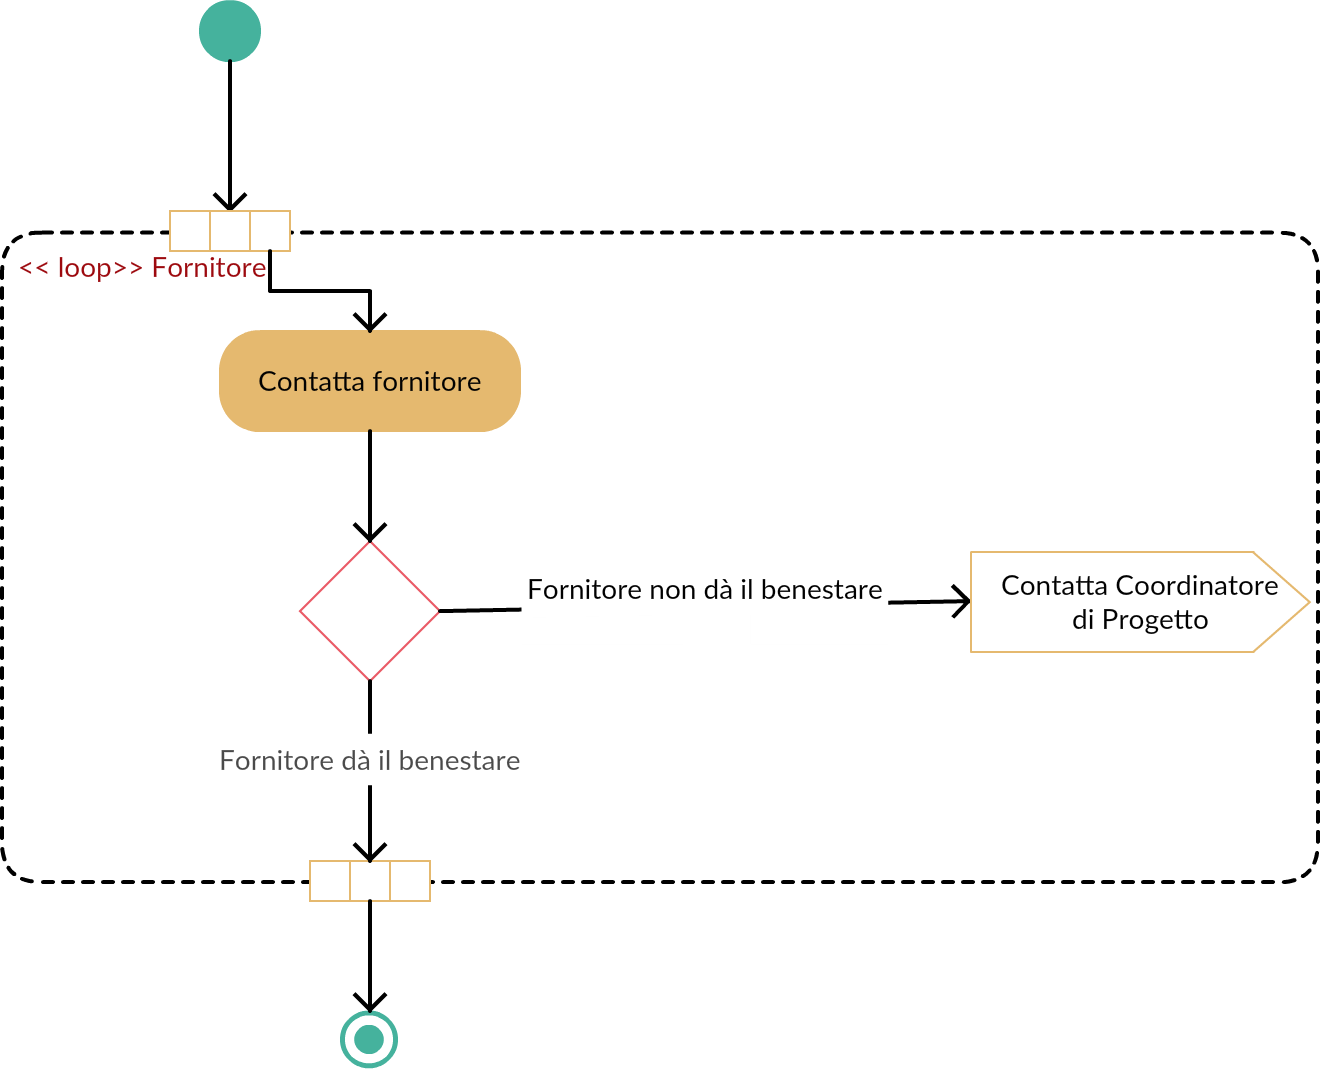
\includegraphics[scale=0.25]{immagini/rollout/contatta-fornitore}
                	\caption{Diagramma di attività del subentro contrattuale.}
				\end{figure}
                
                 \begin{itemize}
               		\item  \textbf{Deliverables:} subentro completato per tutti i contratti esistenti.
                    \item  \textbf{Risorse:} una persona.
                    \item  \textbf{Responsabili:} Capo Progetto.
                    \item  \textbf{Criteri di accettazione:} benestare da parte di tutti i service provider.
                \end{itemize}
            
            
            \subsubsection{Business Process Reengineering (BPR)}
				L'attività di BPR tratta una profonda revisione dei processi aziendali, che ricordiamo essere insiemi di attività correlate che producono valore trasformando degli input in determinati output. La richiesta del Proponente infatti non si limita a richiedere solamente una soluzione tecnologica: il suo obiettivo è la trasformazione del modello aziendale da gerarchico-funzionale a un modello per processi, caratterizzato da una maggiore integrazione.
                \begin{figure}[H]
                  	\centering
                  	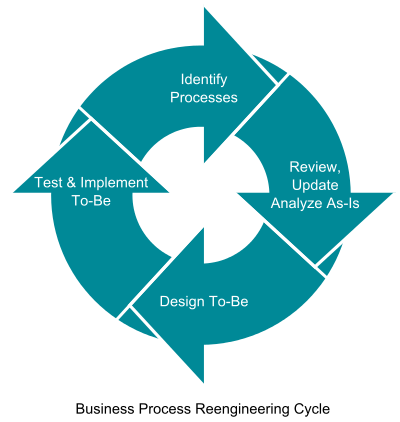
\includegraphics[scale=0.4]{immagini/rollout/BPR}
                	\caption{Ciclo di BPR (\url{https://goo.gl/1Vdufy}).}
				\end{figure}
                Si può suddividere l'attività di BPR in quattro fasi:
                \begin{enumerate}
                	\item \textbf{Identificazione dei processi:} durante questa fase è necessario identificare i processi esistenti (\textit{as-is}) per avere le informazioni di base da cui partire.
                    \item \textbf{Revisione, aggiornamento e analisi dell'as-is:} in questa fase è necessario analizzare in profondità i processi identificati, allo scopo di avere più informazioni possibili.
                    \item \textbf{Design to-be:} in questa fase vengono progettati i nuovi processi, seguendo le linee guida e gli obiettivi del Proponente.
                    \item \textbf{Test e implementazione del to-be}: in quest'ultima fase i processi vengono testati ed effettivamente implementati nella realtà aziendale del Proponente.
                \end{enumerate}
                    
                \begin{itemize}
               		\item  \textbf{Deliverables:} documento Organizzazione dei Processi Aziendali.
                    \item  \textbf{Risorse:} 
                    \begin{itemize}
                    	\item Due persone per l'analisi e lo sviluppo dei processi.
                        \item Due computer portatili.
                        \item Due licenze Microsoft Office.
                    \end{itemize}
                    \item  \textbf{Responsabili:} analisti con conoscenza di processi aziendali.
                    \item  \textbf{Criteri di accettazione:} accettazione da parte del Proponente.
                \end{itemize}

                \subsubsection*{Tasks}
					\begin{enumerate}
						\item \textbf{Osservazione del modo di lavorare presso il Proponente}.\\
                        Per poter analizzare i processi nel dettaglio è necessario presenziare di persona presso la sede del Proponente, per ottenere più informazioni possibili. Il personale dell'Offerente comincerà ad essere presente nella sede del Proponente fin da subito e stilerà relazioni quindicinali su quanto appreso.
					\end{enumerate}
                    
			\subsubsection{Presa in carico sistemi ed erogazione servizi esistenti}  
            	Il Proponente desidera che l'Offerente prenda in carico i sistemi esistenti, prestando parte attiva nell'erogazione dei servizi fin da subito, e non limitandosi esclusivamente allo sviluppo di una soluzione da rilasciare in futuro. 
                \begin{itemize}
                \item \textbf{Deliverables:} 
                	\begin{itemize}
                    	\item Documento Analisi Sistemi.
                    	\item Sistemi presi in carico correttamente.
                        \item Servizi esistenti erogati correttamente.
                    \end{itemize}
                \item  \textbf{Risorse:} 
                \begin{itemize}
                	\item Personale del Centro Gestione Integrato (comprende il Service Desk).
                	\item Hardware esistente presso la sede del Proponente.
                    \item Software esistente presso la sede del Proponente.
                    \item Fornitori attuali del Proponente.
                \end{itemize}
                \item  \textbf{Responsabili:} Personale del Centro Gestione Integrato, Capo Progetto.
                \item  \textbf{Criteri di accettazione:} 
                \begin{itemize}
					\item Test dei sistemi attualmente esistenti.
                    \item Test di erogazione dei servizi esistenti.
                \end{itemize}
                \end{itemize}
                Il seguente diagramma di attività mostra una visione più granulare dell'attività, concentrandosi sulla presa in carico dei sistemi. La presa in carico dei servizi verrà eseguita in modo similare.
                \begin{figure}[H]
					\centering
					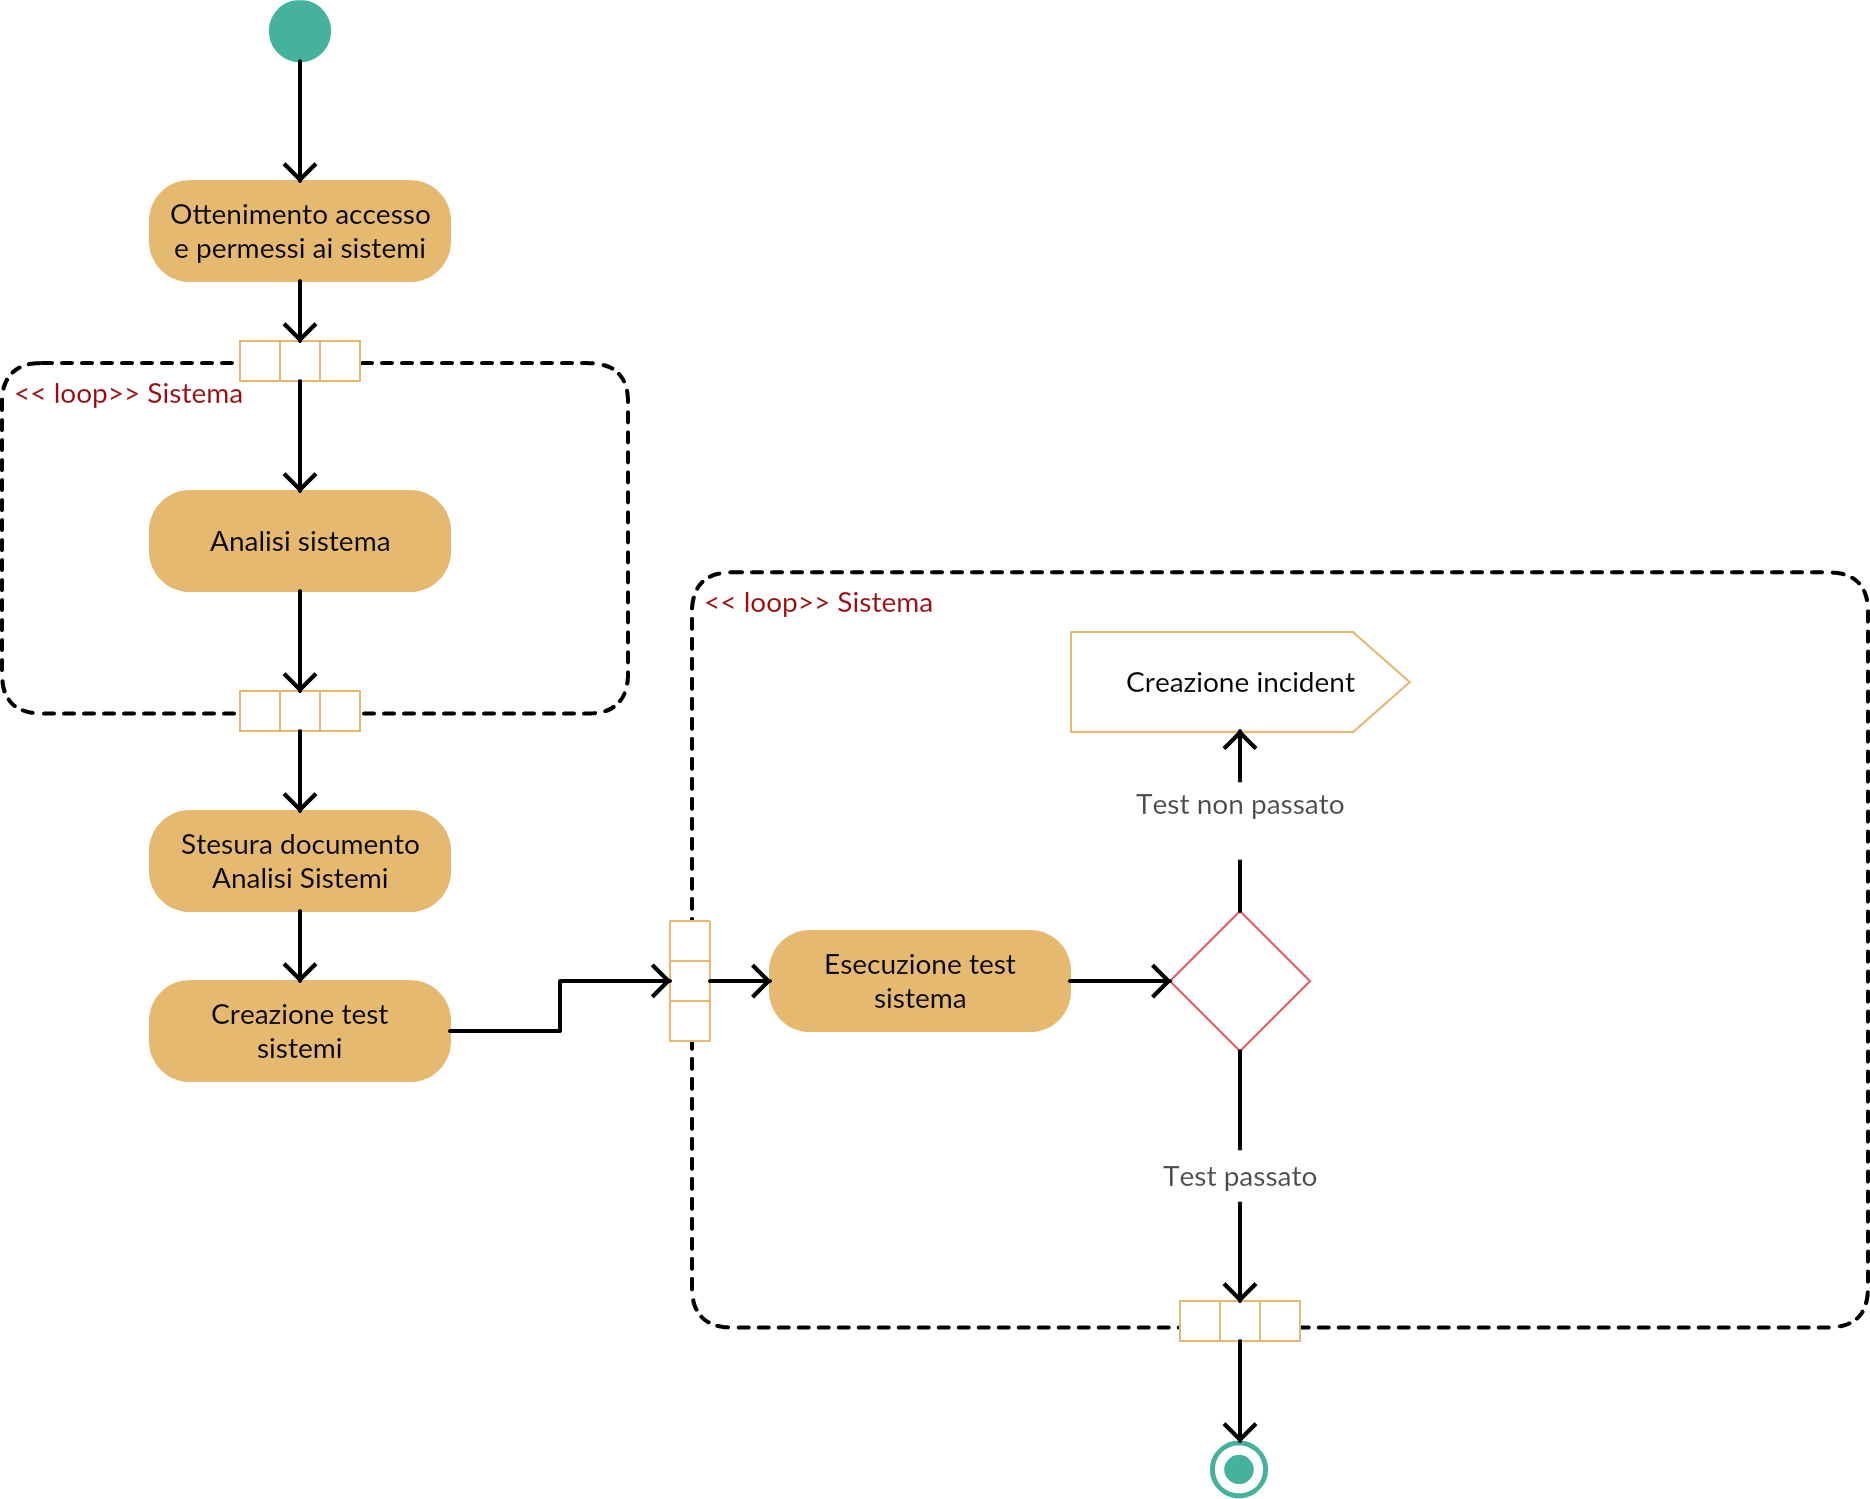
\includegraphics[width=\textwidth]{immagini/rollout/carico-sistemi}
					\caption{Diagramma di attività della presa in carico dei sistemi.}
				\end{figure}
                
                    \subsubsection*{Tasks}
					\begin{enumerate}
                    
                    	 \item \textbf{Ottenimento accesso e permessi di amministratore ai sistemi esistenti}.\\
                         Ottenere l'accesso e i permessi di amministratore per i sistemi esistenti è il primo passo da eseguire.
						\item \textbf{Analisi sistemi esistenti}.\\
                        Analizzare e comprendere i sistemi esistenti presso la sede del Proponente è il passo successivo verso una presa in carico efficace. L'Offerente si occuperà della stesura di un documento di Analisi Sistemi.
                       \item \textbf{Analisi servizi esistenti}.\\
                        Oltre ai sistemi, è necessario analizzare anche i servizi, per comprenderne al meglio le logiche di erogazione.
                       \item \textbf{Test dei sistemi}.\\
                        Prima di poter erogare un servizio l'Offerente vuole accertarsi che i sistemi rispondano correttamente. Per questo motivo, verranno eseguiti dei test per valutare l'adeguatezza di ogni sistema.
                        \item \textbf{Test di erogazione servizi}.\\
                        Una volta essersi assicurati che i sistemi siano adeguati, l'Offerente effettuerà un test di erogazione per ogni servizio, coinvolgendo anche il personale del Proponente.
					\end{enumerate}
                
			\subsubsection{Riprogettazione e reimplementazione Centro Elaborazione Dati (CED)}
				L'Offerente ha scelto di ospitare tutto l'hardware necessario presso il CED del proponente. Tuttavia, il CED ha bisogno di una profonda riprogettazione, sia dal punto di vista hardware, sia per quanto riguarda la messa a norma. L'Offerente non esclude la necessità di interventi strutturali al CED.
                
                \begin{itemize}
               		\item  \textbf{Deliverables:} CED riprogettato e reimplementato.
                    \item  \textbf{Risorse} 
                    \begin{itemize}
                    	\item Due persone per l'analisi, la riprogettazione e la reimplementazione del CED.
                        \item Azienda esterna per interventi strutturali, qualora ce ne fosse bisogno.
                        \item Hardware (porte tagliafuoco, armadi ignifughi, server, ecc) e software necessari.
                	\end{itemize}
                    \item  \textbf{Responsabili:} persone con buone capacità progettuali e conoscenze di networking. 
                    \item  \textbf{Criteri di accettazione:} 
                    \begin{itemize}
                    	\item Test di sistema per valutare la funzionalità del nuovo CED.
                        \item Accettazione da parte del Proponente.
                    \end{itemize}
                \end{itemize}
                
                \subsubsection*{Tasks}
                	\begin{enumerate}
                		\item \textbf{Analisi CED attuale:} analizzare la situazione corrente è fondamentale per capire le funzionalità richieste dal CED.
                        \item \textbf{Progettazione nuovo CED:} dopo che è stata svolta l'analisi, è necessario progettare il nuovo CED, sia dal punto di vista strutturale, sia dal punto di vista di hardware e software.
                        \item \textbf{Esecuzione lavori strutturali:} solo se necessario, dovranno essere eseguiti lavori strutturali (allargamento locale, sistemazione muratura, ecc).
                        \item \textbf{Installazione hardware e software:} verranno installati hardware e software identificati durante la progettazione.
                        \item \textbf{Test del nuovo CED:} verrà eseguito un test dell'intero CED per valutare la corretta implementazione di tutte le funzionalità richieste. Il collaudo verrà eseguito con l'assistenza del personale tecnico dell'U.O. Gestione Tecnico-Patrimoniale, come segnalato nel Capitolato. 
                	\end{enumerate}
                    
			\subsubsection{Personalizzazione e implementazione SAP}
            	L'Offerente ritiene che l'adozione di un ERP sia la soluzione migliore per raggiungere gli obiettivi di integrazione, re-ingegnerizzazione dei processi aziendali e riduzione del numero di applicazioni e sistemi richiesti dal Proponente. L'ERP scelto dall'Offerente è SAP, un software ERP che permette una profonda personalizzazione per meglio adattarlo alla propria realtà e processi aziendali.
                Un software come SAP non è pronto \textit{out-of-the-box}: è necessario eseguire vari passi prima di poterne effettuare il deployment, che verranno descritti dai tasks successivi.
                \begin{itemize}
               		\item  \textbf{Deliverables:} ERP SAP correttamente personalizzato e implementato.
                    \item  \textbf{Risorse:} 
                    \begin{itemize}
                    	\item Tre persone per analisi, progettazione, implementazione e test delle personalizzazioni di SAP.
                        \item Licenze SAP.
                        \item PC, server e sistemi necessari per lo sviluppo e l'installazione di SAP.
                	\end{itemize}
                    \item  \textbf{Responsabili:} analisi, progettisti e programmatori.
                    \item  \textbf{Criteri di accettazione:} 
                    \begin{itemize}
                    	\item Test di sistema di SAP.
                        \item Accettazione da parte del Proponente.
                    \end{itemize}
                \end{itemize}
                
                \subsubsection*{Tasks}
                	\begin{enumerate}
                		\item \textbf{Analisi requisiti:} il primo passo da compiere è analizzare i requisiti e le funzionalità che SAP deve implementare. Più nel dettaglio, dato che il Proponente vuole passare da una situazione con numerosi applicativi ad una con un numero ristretto di applicativi, è necessario analizzare con precisione le funzionalità delle applicazioni attualmente esistenti, per poterle replicare in SAP.
                        \item \textbf{Progettazione personalizzazioni:} dopo aver eseguito l'analisi, è fondamentale progettare le personalizzazioni necessarie.
                        \item \textbf{Implementazione personalizzazioni:} una volta progettate, le personalizzazioni devono essere implementate.
                        \item \textbf{Integrazione CRS-SISS:} date le richieste del Proponente in ambito di integrazione con i progetti sanitari regionali, sarà necessario integrare SAP con il progetto CRS-SISS.
                        \item \textbf{Test di sistema:} una volta completate tutte le attività di implementazione, sarà necessario testare SAP per verificarne la conformità ai requisiti identificati.
                        \item \textbf{Migrazione dati applicativi in SAP:} l'ultimo passo prima di poter utilizzare SAP operativamente è eseguire la migrazione dei dati degli applicativi esistenti.
                	\end{enumerate}
                    
                    
                \subsubsection{Revisione cablaggio e architettura di rete}
	La situazione dell'architettura di rete presso la sede del Proponente presenta diverse problematiche, come tratti con cablaggio a bassa velocità (inferiori al Gigabit) e tratti che bypassano il centro stella, per collegarsi direttamente al CED (come il collegamento dal Servizio Traumatologico d'Urgenza STU).
                    Inoltre, il centro stella risulta attualmente non ridondato, diventando quindi un \textit{single point of failure}.
                    
                    
                    Per ottenere una rete solida, ridondata e senza \textit{single point of failure} sarà necessario eseguire i task descritti più in basso.
                    
                    \begin{itemize}
               		\item  \textbf{Deliverables:} 
                    \begin{itemize}
                    	\item Nuova rete correttamente progettata e implementata.
                        \item Documento Piano di indirizzamento IP e di partizionamento della rete.
                    \end{itemize}
                   
                    \item  \textbf{Risorse} 
                    \begin{itemize}
                    	\item Due persone per analisi, progettazione architettura di rete.
                        \item Azienda esterna per esecuzione lavori di cablaggio e/o ricertificazione fibra, se ritenuto necessario.
						\item Hardware necessario (cavi, router, switch, ecc).
                	\end{itemize}
                    \item  \textbf{Responsabili:} progettisti di rete.
                    \item  \textbf{Criteri di accettazione:} 
                    \begin{itemize}
                    	\item Test di sistema sulla funzionalità di rete.
                        \item Test di ridondanza sulla rete.
                        \item Accettazione da parte del Proponente.
                    \end{itemize}
                	\end{itemize}
                    
                    \subsubsection*{Tasks}
                	\begin{enumerate}
                		\item \textbf{Analisi rete attuale:} il primo passo da eseguire è l'analisi della rete attuale.
                        \item \textbf{Stesura documento Piano di indirizzamento IP e di partizionamento della rete:} questo documento descriverà come l'Offerente intende organizzare l'indirizzamento degli IP e progettare la rete.
                        \item \textbf{Implementazione nuova rete:} sarà necessario eseguire lavori per il cablaggio di nuovi cavi e ricertificazione per quelli esistenti.
                        \item \textbf{Test nuova rete:} sarà necessario infine testare la nuova rete con test che ne verifichino sia la corretta funzionalità che le caratteristiche di ridondanza.
                	\end{enumerate}
                    
                    \subsubsection{Costituzione Centro di Gestione Integrato (CGI)}
                    	Il Proponente desidera la costituzione di un Centro di Gestione Integrato (CGI) presso la propria sede. Lo scopo del CGI è di fornire un servizio dedicato di gestione e assistenza alla struttura ospedaliera.
                        
                        
                        Il CGI sarà composto da:
                        \begin{enumerate}
                        	\item Service Desk.
                            \item Centro di Controllo e Monitoraggio.
                            \item Servizi On-Site per le postazioni di lavoro.
                            \item Risorse in reperibilità notturna e festiva.
                            \item Centro di Supporto per l'Area Direzionale.
                            \item Centro di Supporto per l'Area Gestione Personale.
                        \end{enumerate}
                        
                        
                        \begin{itemize}
               		\item  \textbf{Deliverables:} 
                    \begin{itemize}
                    	\item Centro di Gestione Integrato operativo.
                        \item Documento Organizzazione Centro di Gestione Integrato.
                    \end{itemize}
                                       
                    \item  \textbf{Risorse:} 11 persone in totale, suddivise nel seguente modo: 
                    \begin{itemize}
                    	\item 5 persone per il Service Desk.
                        \item 2 persone per il Centro di Controllo e Monitoraggio.
                        \item 2 persone per i Servizi On-Site per le postazioni di lavoro.
                        \item 2 persone in reperibilità notturna e festiva, a rotazione tra quelle presenti all'interno del CGI.
                        \item 1 persona per il Centro di Supporto per l'Area Direzionale.
                        \item 1 persona per il Centro di Supporto per l'Area Gestione Personale.
                	\end{itemize}
                    \item  \textbf{Responsabili:} 
                    \begin{itemize}
                    	\item Persone con buone capacità di problem solving.
                        \item Persone con buone conoscenze IT per quanto riguarda le postazioni di lavoro.
                        \item Persone con conoscenze di management per il supporto all'area direzionale.
                        \item Persone con conoscenze in ambito di gestione personale.
                    \end{itemize}
                    \item  \textbf{Criteri di accettazione:} 
                    \begin{itemize}
                        \item Accettazione da parte del Proponente.
                    \end{itemize}
                	\end{itemize}
                
                    \subsubsection{Presa in carico postazioni di lavoro}
                    	Le postazioni di lavoro attualmente presenti presso la sede del Proponente sono estremamente variabili per quanto riguarda marca e anno di acquisto. Inoltre, le informazioni riguardo la marca per alcune postazioni di lavoro risultano non essere disponibili: questo è sintomo di un processo di Service Asset and Configuration Management svolto in maniera non ottimale.
                        
                        
                        L'Offerente desidera prendere in carico, come richiesto, la gestione delle postazioni di lavoro, risolvendo le problematiche segnalate e successivamente controllando e sostituendo regolarmente le postazioni di lavoro.
                        
                        
                        Il diagramma di attività sottostante mostra il flusso di lavoro della sostituzione di una postazione di lavoro. Il diagramma per sostituzione stampanti e altro hardware è similare, con l'accortezza di cambiare il limite temporale da prendere in considerazione per la sostituzione.
                        \begin{figure}[H]
							\centering
							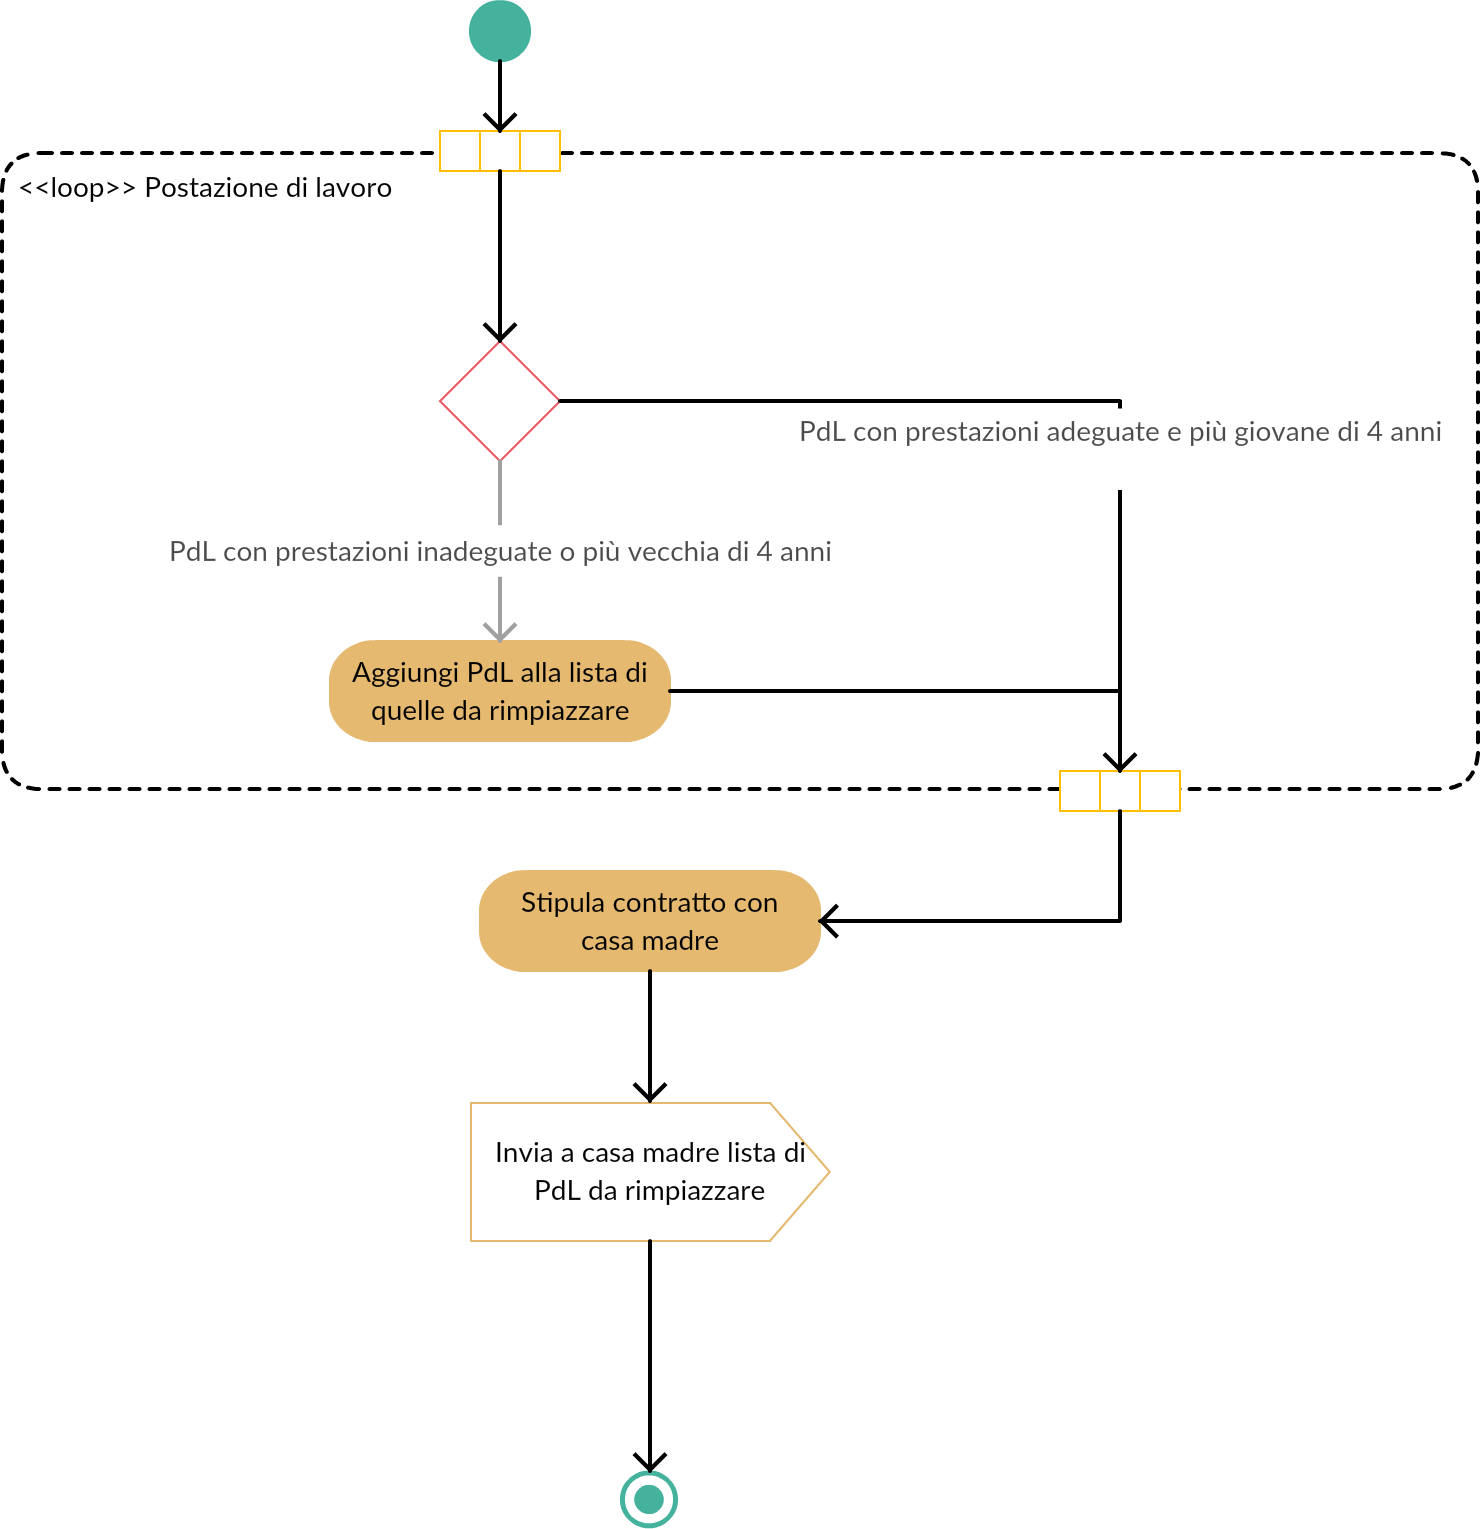
\includegraphics[scale=0.237]{immagini/rollout/sostituzione-pdl}
							\caption{Diagramma di attività sostituzione PdL.}
							\end{figure}
                        
                        
                        
                         \begin{itemize}
               		\item  \textbf{Deliverables:} 
                    \begin{itemize}
                    	\item Postazioni di lavoro troppo vecchie o inadeguate rimpiazzate.
                        \item Postazioni di lavoro gestite completamente dall'Offerente.
                    \end{itemize}
                                       
                    \item  \textbf{Risorse:} 
                	\begin{itemize}
                		\item Postazioni di lavoro, stampanti e altro hardware e software necessari. 
                        \item Azienda esterna (casa madre) che si occupi dell'installazione e manutenzione.
                	\end{itemize}
                    \item  \textbf{Responsabili:} azienda esterna (casa madre).
                    \item  \textbf{Criteri di accettazione:} 
                    \begin{itemize}
                    	\item Nessuna postazione di lavoro più vecchia di 4 anni rimanente.
                        \item Nessuna stampante a getto d'inchiostro o ad aghi più vecchia di 18 mesi rimanente.
                        \item Nessuna stampante laser più vecchia di 2 anni rimanente.
                        \item Nessuna stampante laser dipartimentale più vecchia di 4 anni rimanente.
                    \end{itemize}
                	\end{itemize}
                    
                    \subsubsection*{Tasks}
                    \begin{enumerate}
                    	\item \textbf{Identificazione postazioni di lavoro da sostituire:} è necessario identificare le PdL con prestazioni inadeguate o troppo vecchie e aggiungerle alla lista per la sostituzione.
                        \item \textbf{Stipulazione contratto:} è necessario stipulare un contratto con una ditta esterna (possibilmente casa madre) per l'acquisto, l'installazione e la manutenzione delle PdL da sostituire.
                    \end{enumerate}
                    
			\subsubsection{Sviluppo progetti innovativi}
            	Il Proponente, con lo scopo di mantenere alto il proprio livello di competitività e innovazione tecnologica, richiede lo sviluppo di progetti innovativi. Dato che questi progetti possono richiedere tecnologie innovative, l'Offerente prevede di appoggiarsi anche a figure come ricercatori e dottorandi nella fase di ideazione.
                
                \begin{itemize}
               		\item  \textbf{Deliverables:} 
                    \begin{itemize}
                    	\item Progetti innovativi sviluppati e implementati correttamente.
                        \item Documento Progetti Innovativi.
                    \end{itemize}
                                       
                    \item  \textbf{Risorse:} 
                	\begin{itemize}
                		\item 2 persone quali dottorandi e ricercatori per la fase di ideazione.
                        \item 3 persone interne all'Offerente per progettazione e implementazione.
                	\end{itemize}
                    \item  \textbf{Responsabili:} figure con buone capacità innovative e mente aperta.
                    \item  \textbf{Criteri di accettazione:} 
                    \begin{itemize}
                    	\item Test di sistema per ogni progetto innovativo.
                        \item Accettazione da parte del proponente.
                    \end{itemize}
                	\end{itemize}
                    
                    \subsubsection*{Tasks}
                    \begin{enumerate}
                    	\item \textbf{Identificazione figure esterne:} come primo passo l'Offerente desidera identificare figure quali dottorandi e ricercatori per l'ideazione dei progetti innovativi.
                        \item \textbf{Brainstorming:} le figure esterne e il team dell'Offerente dovranno eseguire un brainstorming per l'identificazione delle idee innovative.
                        \item \textbf{Scelta idee:} una volta identifica le idee, devono essere valutate e infine scelte quelle ritenute migliori, coinvolgendo anche il Proponente.  
                        \item \textbf{Progettazione:} sarà necessario progettare le soluzioni innovative.
                        \item \textbf{Implementazione:} successivamente alla progettazione, sarà necessario implementare quanto progettato.
                        \item \textbf{Test:} infine, bisognerà testare le soluzioni innovative implementate.
                    \end{enumerate}
                    
                    
			\subsubsection{Stesura documentazione preliminare}
            	Il Proponente richiede la presentazione di documentazione preliminarmente all'assegnazione dell'appalto. La stesura di questa documentazione è molto importante dato che l'Offerente verrà scelto in base al grado di dettaglio, chiarezza e precisione della documentazione.
                
                
                La stesura della documentazione sarà supervisionata dal Capo Progetto.
                \begin{itemize}
               		\item  \textbf{Deliverables:} 
                    \begin{itemize}
                    	\item Documento Presentazione dell'Impresa.
                        \item Documento Progetto Organizzativo.
                        \item Documento Progetto Applicativo.
                        \item Documento Progetto Tecnologico.
                        \item Documento Progetto delle sperimentazioni e delle proposte innovative.
                        \item Documento Progetto di Erogazione e Gestione del Servizio.
                        \item Documento Pianificazione generale.
                    \end{itemize}
                                       
                    \item  \textbf{Risorse:} 
                	\begin{itemize}
                		\item 3 analisti.
                        \item 2 progettisti.
                        \item Capo Progetto.
                	\end{itemize}
                    \item  \textbf{Responsabili:} analisti, progettisti e capo progetto.
                    \item  \textbf{Criteri di accettazione:} 
                    \begin{itemize}
                    	\item Accettazione da parte del Capo Progetto.
                    \end{itemize}
                	\end{itemize}
                    
					\subsubsection*{Tasks}
                    \begin{enumerate}
                    	\item \textbf{Stesura Presentazione dell'Impresa}.
                        \item \textbf{Stesura Progetto Organizzativo}.
                        \item \textbf{Stesura Progetto Applicativo}.
                        \item \textbf{Stesura Progetto Tecnologico}.
                        \item \textbf{Stesura Progetto delle sperimentazioni e delle proposte innovative}.
                        \item \textbf{Stesura Progetto di Erogazione e Gestione del Servizio.}.
                        \item \textbf{Stesura Pianificazione generale}.
                    \end{enumerate}
                    
			\subsubsection{Realizzazione soluzione di continuità}
            	L'Offerente intende garantire la Business Continuity realizzando una soluzione come descritta nel capitolo 2. La soluzione di continuità verrà implementata man mano che i servizi e i sistemi della nuova soluzione andranno live.
                
                
                Maggiori dettagli sull'implementazione della soluzione sono presenti nella sezione \ref{ScadenzaContinuità}.
                
                \begin{itemize}
               		\item  \textbf{Deliverables:} 
                    \begin{itemize}
                    	\item Soluzione di continuità implementata e testata correttamente.
                        \item Sito di Disaster \& Recovery attivo.
					\end{itemize}    
                    \item  \textbf{Risorse:} 
                	\begin{itemize}
                		\item 2 analisti.
                        \item 2 progettisti.
                        \item 1 sistemista.
                        \item Capo Progetto.
                	\end{itemize}
                    \item  \textbf{Responsabili:} analisti, progettisti, sistemisti e Capo Progetto.
                    \item  \textbf{Criteri di accettazione:} 
                    \begin{itemize}
                    	\item Superamento test di sistema.
                    	\item Accettazione da parte del Capo Progetto.
                    \end{itemize}
                	\end{itemize}
                    
					\subsubsection*{Tasks}
                    \begin{enumerate}
                    	\item \textbf{Analisi}.
                        \item \textbf{Progettazione}.
                        \item \textbf{Implementazione}.
                        \item \textbf{Test}.
                    \end{enumerate}
                    
			\subsubsection{Test periodico soluzione di continuità}
            	L'Offerente intende effettuare dei test annuali per garantire l'efficacia operativa della soluzione di continuità. Maggiori dettagli riguardo questi test sono stati descritti nel capitolo 2. 
                
                \begin{itemize}
               		\item  \textbf{Deliverables:} 
                    \begin{itemize}
                    	\item Soluzione di continuità testata correttamente.
                        \item Documento Esito test soluzione di continuità.
					\end{itemize}    
                    \item  \textbf{Risorse:} 
                	\begin{itemize}
                		\item 2 sistemisti.
                	\end{itemize}
                    \item  \textbf{Responsabili:} sistemisti.
                    \item  \textbf{Criteri di accettazione:} 
                    \begin{itemize}
                    	\item Superamento test di sistema.
                    \end{itemize}
                	\end{itemize}
                    
					\subsubsection*{Tasks}
                    \begin{enumerate}
                    	\item \textbf{Test soluzione di continuità}.
                    \end{enumerate}
                    
                    
		\subsection{Pianificazione dell'implementazione e milestones}
        	In questa sezione verrà presentata una pianificazione temporale delle attività identificate nella sezione precedente. Ad ogni attività verrà assegnata:
            \begin{itemize}
            	\item Data d'inizio.
                \item Data di fine.
                \item Durata.
            \end{itemize}
            Inoltre verranno identificate alcune \textit{milestones}, ovvero dei traguardi intermedi importanti per lo svolgimento del progetto.
            
            
            Per motivi di semplicità di rappresentazione, si assumerà che la firma del contratto e la data di verbale di inizio progetto avvengano in data 01/01/n. Naturalmente le attività di redazione di documentazione preliminare e analisi tramite sopralluoghi inizieranno prima della data di presa in carico.
            
            
            Le \textit{milestones} sono identificate tramite dei riquadri sotto il completamento di alcune attività. 
            
            
            \begin{figure}[H]
				\centering
				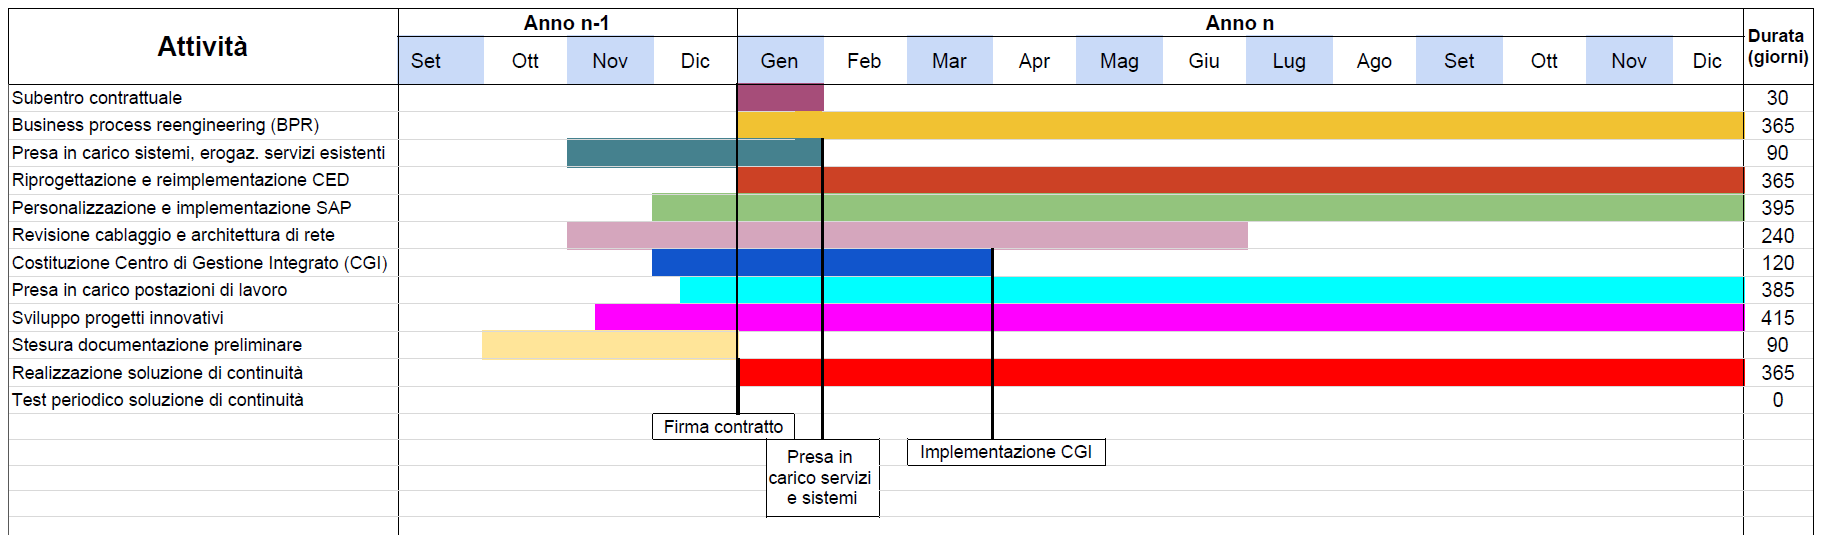
\includegraphics[width=\textwidth]{immagini/rollout/gantt-a1}
				\caption{Gantt anno n-1 e n.}
			\end{figure}
            
            \begin{figure}[H]
				\centering
				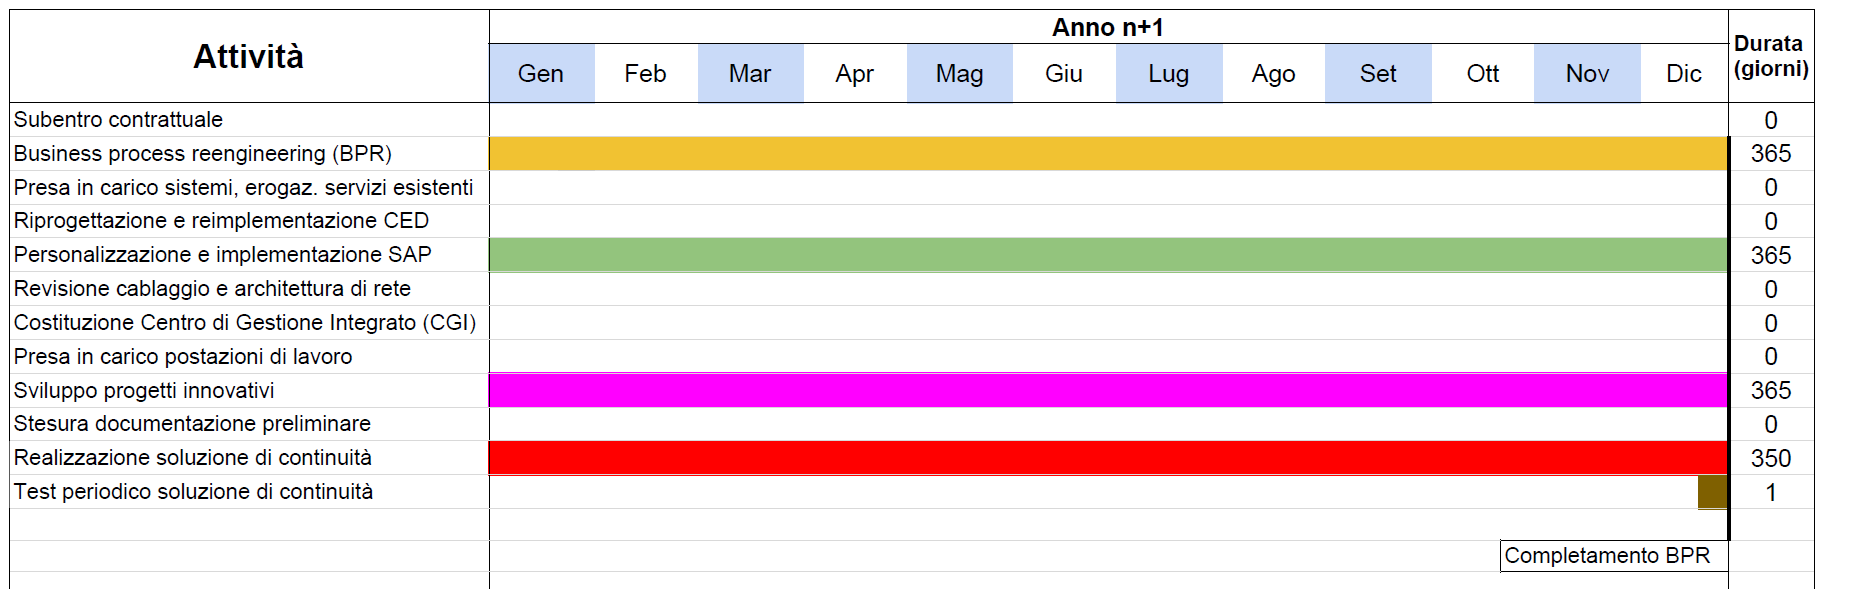
\includegraphics[width=\textwidth]{immagini/rollout/gantt-a2}
				\caption{Gantt anno n+1.}
			\end{figure}
            
            \begin{figure}[H]
				\centering
				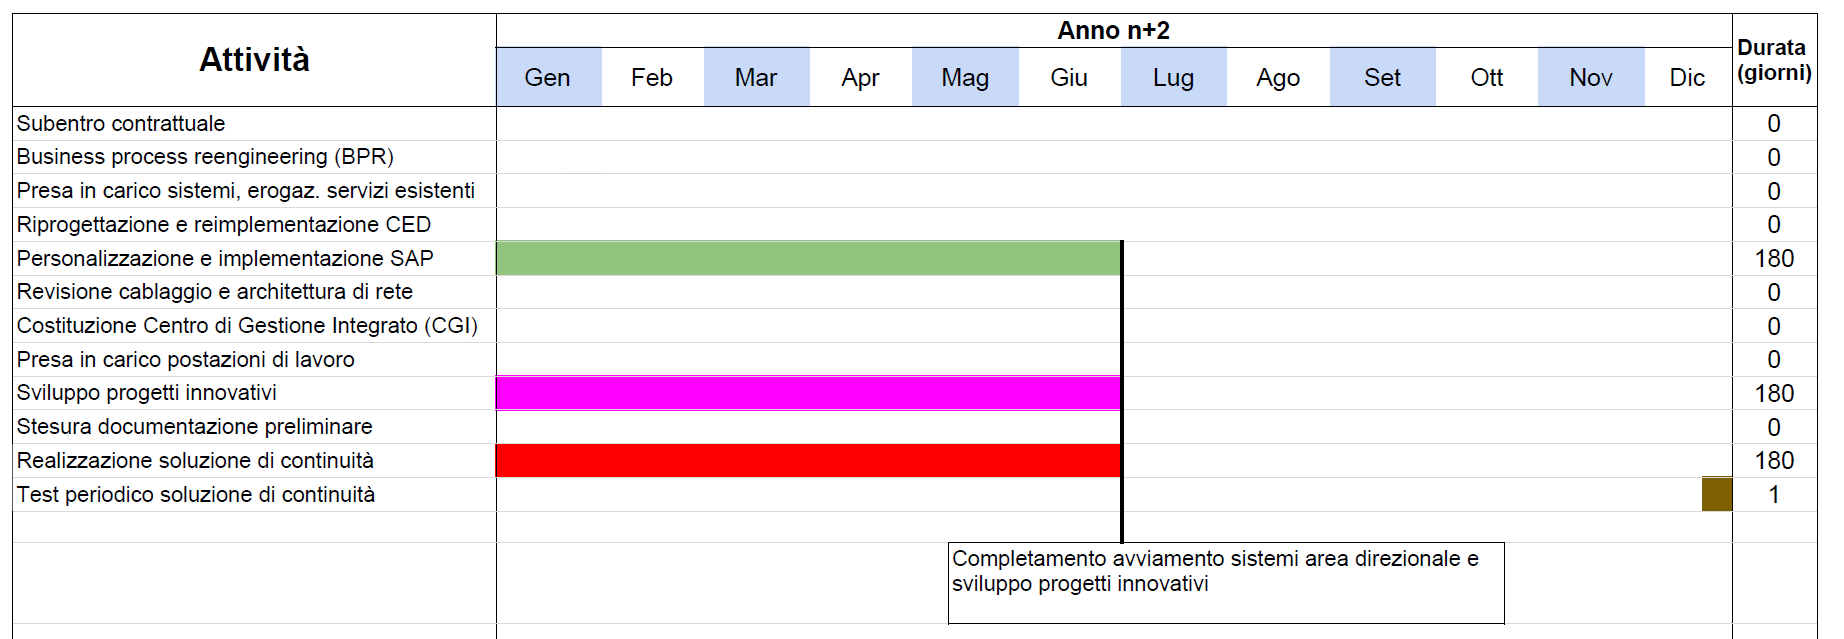
\includegraphics[width=\textwidth]{immagini/rollout/gantt-a3}
				\caption{Gantt anno n+2.}
			\end{figure}
                    
                    
		\subsection{Privacy e sicurezza}
                    In questa sezione verranno trattati requisiti, problematiche e soluzioni relative alla privacy e alla sicurezza durante la fase di rollout. In particolare, dato che durante la migrazione dai vecchi sistemi ai nuovi dovranno essere migrati anche i dati personali relativi ai dipendenti, il tema privacy assume un ruolo di fondamentale importanza.
                    
                    \subsubsection{Privacy}
                    
                    Dall'entrata in vigore del nuovo Regolamento sulla privacy del 25 maggio 2018 sono stati stabiliti obblighi stringenti e nuove responsabilità rispetto al precedente Codice della privacy con lo scopo di tutelare e salvaguardare i dati personali delle persone fisiche.
                
                
                	Il primo punto fondamentale da considerare è il \textbf{consenso} del soggetto di cui si stanno trattando i dati. Il consenso dev'essere sempre preventivo e inequivocabile, escludendo ogni ipotesi di consenso tacito. Dato che al momento della firma del contratto il Proponente tratta già i dati personali dei propri dipendenti, si presuppone che il consenso sia stato chiesto preventivamente all'assunzione. Tuttavia l'Offerente, in fase di migrazione, desidera confermare che tale consenso sia stato espresso in maniera esplicita, e sanando ogni discrepanza in caso non lo sia stato.
                    
                    
                    Il secondo punto da considerare è il \textbf{data breach}: in caso di violazioni esterne, come ad esempio attacchi hacker o furti di dischi, l'Offerente, in qualità di titolare del trattamento, dovrà comunicare il fatto al Garante nazionale e anche al soggetto interessato, nel caso in cui la violazione rappresenti una minaccia per i suoi diritti o le sue libertà. Sarà quindi necessario informare i membri del team dell'Offerente che verranno a contatto con dati personali di questa procedura, istruendoli sui passi necessari per trattare correttamente questo caso.
                    
                    
                    Come descritto nel regolamento, l'Offerente desidera seguire i principi di \textbf{privacy by default} e \textbf{privacy by design}. Secondo il primo principio, l'Offerente deve tutelare la privacy di default all'interno dell'organizzazione aziendale, dotandosi di sistemi opportuni. Per adempiere a ciò, l'Offerente memorizzerà i dati sensibiili all'interno di database protetti da password. La password verrà divulgata solamente ai soggetti che necessitano di conoscerla, seguendo il principio "\textbf{need to know}". L'accesso ai dati da parte di soggetti che non hanno bisogno di conoscere la password avverrà tramite apposite interfacce e maschere, con lo scopo di divulgare i dati personali nella minima quantità possibile.
                    
                    
                    Per quanto riguarda il secondo principio, \textbf{privacy by design}, il titolare dei dati deve proteggere i dati fin dalla progettazione di un applicativo o di un processo aziendale.  L'Offerente intende seguire in modo completo questo principio, progettando processi e applicativi di conseguenza. Per raggiungere questo scopo, si prevede un'analisi dei rischi legati al trattamento dei dati prima di eseguire le attività di progettazione. L'identificazione dei rischi sarà utile per evitare il verificarsi degli stessi.

					
                    Il Capo Progetto ricoprirà il ruolo di \textbf{Responsabile della Protezione dei Dati Personali (Dpo)}, data la sua grande esperienza e competenza, allo scopo di minimizzare i rischi dovuti al mancato rispetto del Regolamento sulla privacy.
                	
					\subsubsection{Sicurezza}
						Oltre alla privacy, un'altra componente che è necessario assicurare è la sicurezza. Dal punto di vista ITIL, la sicurezza (\textit{security}) è composta da:
                        \begin{itemize}
                        	\item \textbf{Confidentiality}.
                            \item \textbf{Integrity}.
                            \item \textbf{Availability}.
                        \end{itemize}
                        A differenza della privacy, che tende ed essere orientata ai processi, basata su ambito legale e la cui risposta alle violazioni è consiste tipicamente in una notifica, la security:
                        \begin{itemize}
                        	\item Si basa principalmente su ambito IT.
                            \item È orientata agli strumenti e alle tecnologie.
                            \item Risponde alle violazioni con contenimenti e correzioni.
                        \end{itemize}
                        L'Offerente, durante il rollout e la conduzione del progetto presso il Proponente, desidera seguire lo standard ISO 27001:2013 e seguenti, che documentano i requisiti e forniscono supporto per l'implementazione di un Information Security Management System (ISMS). Più nel dettaglio, ISO 27001 stabilisce che il management debba:
                        \begin{itemize}
                        	\item Sistematicamente esaminare i rischi di sicurezza.
                            \item Progettare e implementare meccanismi di controllo.
                            \item Adottare un processo di management globale.
                        \end{itemize}
                        L'adozione di un tale approccio permette l'identificazione tempestiva e la risoluzione dei rischi che rischiano di violare la sicurezza, aumentando contemporaneamente la credibilità nei confronti degli stakeholder.
                        Ulteriori dettagli implementativi esulano dallo scopo di questo documento e dovrebbero essere trattati dal processo di Information and Security Management (ISM).

\newpage

	\section{Supporto all'implementazione}
    	Questa sezione descrive le risorse necessarie per supportare l'implementazione, intese come hardware, software, strutture, materiali, documenti, personale e requisiti di formazione, rischi, problematiche e impatti implementativi sull'ambiente corrente.
        
        \subsection{Hardware, software e strutture}
			In questa sezione sono elencati hardware, software e strutture di supporto che l'Offerente utilizzerà l'implementazione del progetto. Più nello specifico, verranno indicati gli strumenti necessari all'Offerente per lo sviluppo delle soluzioni. Verranno tralasciati i modelli specifici per quanto riguarda l'hardware.
            \subsubsection{Hardware}
            	L'hardware necessario per l'implementazione è:
                \begin{itemize}
                	\item 10 PC di buone prestazioni per lo sviluppo degli applicativi (personalizzazioni SAP) e la stesura di documentazione.
                    \item 10 notebook di buone prestazioni per poter lavorare in mobilità.
                    \item Due server.   
                    \item Ulteriore hardware necessario all'implementazione della soluzione presso la sede del Proponente.
                \end{itemize}
                
            \subsubsection{Software}
            	Il software necessario per l'implementazione è:
            		\begin{itemize}
            			\item 20 licenze di Microsoft Office.
                        \item 20 licenze di Microsoft Windows 10.
                        \item 5 licenze Debian.
                        \item 5 licenze di kit di sviluppo software SAP per l'implementazione delle personalizzazioni.
                        \item 5 licenze Creately (sviluppo diagrammi UML).
                        \item Ulteriore software necessario all'implementazione della soluzione presso la sede del Proponente.
            		\end{itemize}
                    
            \subsubsection{Strutture}
            	Le strutture necessarie per l'implementazione sono:
               	\begin{itemize}
               		\item Sede dell'Offerente, con orari 9-13 e 14-18, lunedì-venerdì.
                    \item Sede del Proponente con orari 9-13 e 14-18, lunedì-venerdì.
               	\end{itemize}

			\subsection{Documentazione}
            	Durante l'implementazione del progetto sarà necessario produrre la seguente documentazione:
                \begin{itemize}
                	\item Organizzazione dei Processi Aziendali.
					\item Analisi sistemi.
					\item Piano di indirizzamento IP e di partizionamento della rete.
					\item Organizzazione Centro di Gestione Integrato.
					\item Progetti innnovativi.
					\item Documentazione quindicinale per documentare l'avanzamento del progetto.
                    \item Documenti di esito dei test annuali di continuità.
                \end{itemize}
                
			\subsection{Personale}
            	In questa sezione verrà descritto il personale necessario per l'implementazione del progetto.
                
                \subsubsection{Requisiti di staff}
                	Il personale richiesto per l'implementazione del progetto è il seguente:
                    \begin{itemize}
                    	\item 11 persone per la costituzione del Centro di Gestione Integrato presso la sede del Proponente.
                        \item 3 analisti.
                        \item 2 progettisti.
                        \item 3 programmatori.
                        \item 2 amministratori di sistema.
                        \item 2 ricercatori o dottorandi per analisi e brainstorming riguardo progetti innovativi.
                        \item 1 capo progetto.
                    \end{itemize}
				
                \subsubsection{Formazione dello staff}
                	\begin{itemize}
                		\item \textbf{Formazione staff Centro Gestione Integrato:} la formazione dello staff del CGI, che ricordiamo lavorerà stabilmente presso la sede del Proponente, verrà eseguito in maniera differente rispetto a quella degli altri membri del team. Dato che i membri del CGI devono rispondere efficacemente alle richieste degli utenti agendo da \textit{single point of contact} e affiancare il Proponente nella gestione quotidiana di vari compiti, l'Offerente desidera che il CGI sia costituito da personale altamente professionale. 
                        
                        
                        Allo scopo di formare questo personale, l'Offerente richiede che tutti i membri del CGI conseguano almeno la \textbf{certificazione ITIL Foundations} per dimostrare la propria conoscenza dei processi ITIL. Inoltre, saranno valutate positivamente altre certificazioni in campo informatico, come ad esempio la CompTIA A+. I membri saranno scelti tra candidati con buone capacità relazionali e soft skills, dando priorità a figure con esperienza pregressa in ruoli di service desk.
                        
                        
                        Ogni membro del CGI verrà messo a conoscenza dei processi aziendali del Proponente esistenti durante la presa in carico. Inoltre, prima della conclusione dell'attività di \textbf{Business Process Reengineering}, i membri del CGI verranno formati nuovamente, spiegando loro i nuovi processi.
                        
                        
                        L'Offerente sottoporrà ogni candidato membro del CGI ad un \textbf{test di valutazione}, sia in fase di presa in carico che prima della conclusione del BPR, per verificare la sua comprensione dei processi aziendali.
                        
                        
                        La formazione iniziale è stimata in 40 ore. Il personale del CGI continuerà ad essere formato anche dopo la presa in carico con regolari sessioni di formazione mensili, o straordinarie in caso di necessità. Allo scopo di rispettare gli SLA del service desk, le sessioni di formazione regolari saranno tenute dopo l'orario di lavoro, in modo da non lasciare il service desk completamente scoperto, compensando adeguatamente il personale.
                        
                        Le sessioni regolari di formazione, della durata di \textbf{1 ora}, seguiranno la seguente pianificazione:
                        \begin{itemize}
                        	\item Annunci: 5 minuti.
                            \item Discussione: 10 minuti.
                            \item Attività di soft skill: 15 minuti.
                            \item Formazione tecnica: 30 minuti.
                        \end{itemize}
                        
                        \item \textbf{Formazione di staff esterno al CGI:} l'implementazione del progetto richiede l'impiego di staff esterno al CGI, che consisterà in personale che lavora presso l'Offerente, già formato ed esperto nello sviluppo di soluzioni nell'ambito IT. Alla luce di questo, l'Offerente non prevede l'esecuzione di attività di formazione tecnica per lo staff esterno al CGI.


Tuttavia, ai fini di garantire il rispetto della privacy e della continuità, il personale verrà formato:
\begin{itemize}
	\item Inizialmente, con formazione di 20 ore, e continuativamente, ogni 6 mesi con sessioni di 2 ore, per la privacy.
    \item Continuativamente come indicato nella sezione \ref{ScadenzaContinuità} per la continuità.
\end{itemize}
\end{itemize}
                    
			\subsection{Rischi e problemi noti}
            	In questa sezione verranno esposti rischi, problemi, restrizioni o limitazioni che devono essere tenuti in considerazione durante lo sviluppo del progetto. Per i rischi verranno inoltre descritte delle contromisure che, da una prima analisi, risultano essere utili a diminuire il rischio residuo. 
                
                
                Nonostante questa sezione non voglia condurre un'analisi approfondita del rischio, obiettivo del processo di Risk Management, l'Offerente ritiene importante identificare i rischi che potrebbero impattare il processo di implementazione.
                
                \begin{figure}[H]
				\centering
				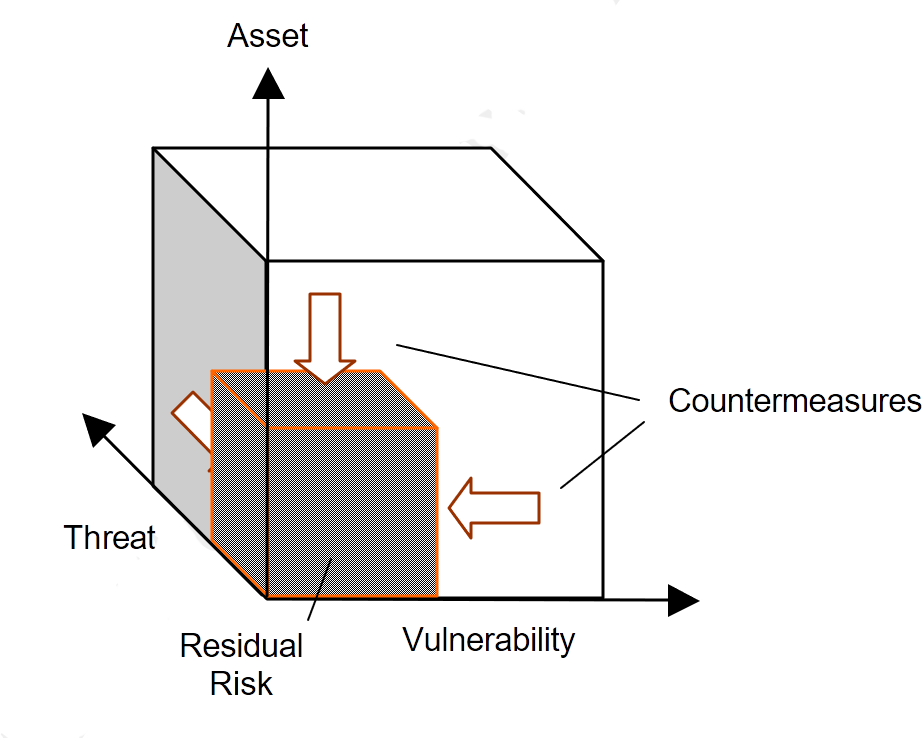
\includegraphics[scale=0.3]{immagini/rollout/risk}
				\caption{Rappresentazione del rischio (\url{https://goo.gl/iBomQ7}).}
			\end{figure}
                
                Ricordando la definizione di rischio definita dal \textbf{CRAMM}, ovvero il prodotto tra valore dell'\textbf{asset}, \textbf{minaccia} e \textbf{vulnerabilità}, nel seguito verrà svolta un'analisi semplificata, non tenendo in considerazione il valore dell'asset nel calcolo del rischio.
                
                
                Per ogni rischio verranno quindi specificati: 
                \begin{itemize}
                	\item \textbf{Livello di rischio}: indica il livello del rischio prima dell'adozione delle contromisure.
                    \item \textbf{Livello di rischio residuo:} indica il livello del rischio dopo l'adozione delle contromisure.
                \end{itemize}
                
                
                Adottando una misura qualitativa, ogni livello di rischio assumerà uno dei seguenti valori:
                \begin{itemize}
                	\item Alto: rischio alto, grave impatto sul business.
                    \item Medio: rischio medio, moderato impatto sul business.
                    \item Basso: rischio basso, piccolo impatto sul business.
                \end{itemize}
                
                
                \subsubsection{Ambiente ospedaliero}
                	È fondamentale tenere in considerazione che il team dell'Offerente dovrà implementare la soluzione progettata in un ambiente ospedaliero. Questo significa lavorare in un ambiente affollato, rumoroso e potenzialmente difficile da navigare. Il rischio maggiore è quello di intralciare le attività di medici e pazienti.
                    \begin{itemize}
                    	\item \textbf{Livello di rischio:} medio.
                        \item \textbf{Contromisure:} 
                        \begin{itemize}
                        	\item Informare medici e personale dell'ospedale delle attività che verranno eseguite.
                            \item Installare cartelli e altro materiale informativo nei pressi delle zone più pericolose, come il CED o corridoi molto frequentati.
                            \item Rispettare i regolamenti di sicurezza sul luogo di lavoro.
                            \item Eseguire le attività più "distruttive" in orari di bassa o nulla frequentazione, ad esempio evitando gli orari in cui sono permesse le visite.
                        \end{itemize}
                        \item \textbf{Livello di rischio residuo:} basso.
                    \end{itemize}
                    
				\subsubsection{Informazioni personali}
                	Come già descritto precedentemente, durante la migrazione l'Offerente verrà a contatto con informazioni personali di persone fisiche, ad esempio quelle del personale dell'ospedale e dei pazienti. Un eventuale data breach potrebbe avere conseguenze molto gravi, sia dal punto di vista legale che di immagine.
                    \begin{itemize}
                    	\item \textbf{Livello di rischio:} alto.
                        \item \textbf{Contromisure:} 
                        \begin{itemize}
                        	\item Limitare gli accessi ai dati sensibili seguendo il principio \textit{need to know}.
                            \item Proteggere i dati sensibili con password sicure.
                            \item Cambiare tali password una volta al mese.
                            \item Assicurarsi di limitare l'accesso fisico ai locali con apposite misure di sicurezza.
                            \item Controllare il background del personale che ha diritto all'accesso ai dati sensibili.
                        \end{itemize}
                        \item \textbf{Livello di rischio residuo:} medio.
                    \end{itemize}
                    
				\subsubsection{Interruzione del servizio}
                	All'Offerente viene richiesto di prendere in carico completamente la gestione del sistema informativo del Proponente, passando da una situazione frammentata con molti applicativi e sistemi ad una integrata, limitando il numero di questi elementi. Durante l'implementazione del progetto, e soprattutto durante la fase di migrazione dai vecchi sistemi al nuovo, c'è il rischio che si verifichi un'interruzione del servizio. Una tale eventualità potrebbe avere vari livelli di gravità, considerando le penali qualora si violassero gli SLA e anche i danni di immagine se l'interruzione dovesse causare danno a qualche paziente.
                    \begin{itemize}
                    	\item \textbf{Livello di rischio:} alto.
                        \item \textbf{Contromisure:} 
                        \begin{itemize}
                        	\item Pubblicizzare con largo anticipo (almeno 30 giorni) la data di migrazione da un sistema vecchio ad uno nuovo.
                            \item Concordare con il Proponente gli orari di down dei servizi per effettuare la migrazione.
                            \item Effettuare la migrazione quando tali servizi non sono in uso.
                            \item Sviluppare dei piani di rollback per ogni sistema nel caso in cui la migrazione non avesse successo.
                        \end{itemize}
                        \item \textbf{Livello di rischio residuo:} medio.
                    \end{itemize}
                    
				\subsubsection{Indisponibilità di risorse umane}
                	Per l'implementazione della soluzione sono necessarie le risorse umane indicate precedentemente. Il rischio riguarda la possibilità che alcune risorse umane non siano disponibili per qualche periodo a causa di motivi vari, come ad esempio problemi di salute. Se questa situazione si prolunga per lungo tempo si potrebbero avere ritardi di implementazione.
                    \begin{itemize}
                    	\item \textbf{Livello di rischio:} medio.
                        \item \textbf{Contromisure:} 
                        \begin{itemize}
                        	\item Attingere al personale residuo dell'Offerente, che si presume non starà lavorando sul progetto, in caso di indisponibilità di uno o più membri del team. Il personale di riserva dev'essere disponibile in misura del 10\% delle dimensioni del team.
                            \item Restare in contatto con candidati e agenzie di collocamento in modo da trovare dei sostituti in caso di indisponibilità di lungo periodo. 
                        \end{itemize}
                        \item \textbf{Livello di rischio residuo:} basso.
                    \end{itemize}
                    
				\subsubsection{Indisponibilità di risorse hardware}
                	Per lo sviluppo e l'implementazione della soluzione sono necessarie numerose risorse hardware, sia di proprietà dell'Offerente, utilizzate per lo sviluppo delle soluzioni, sia risorse nuove da acquistare, come postazioni di lavoro, switch, router e server. 
                    
                    
                    Il rischio consiste nell'indisponibilità di risorse sia per quanto riguarda l'Offerente, sia per quanto riguarda l'hardware che si deve acquistare.
                    \begin{itemize}
                    	\item \textbf{Livello di rischio:} medio.
                        \item \textbf{Contromisure:} 
                        \begin{itemize}
                        	\item Stipulare un contratto per la fornitura di hardware (postazioni di lavoro, server, ecc) a richiesta presso la sede dell'Offerente in tempi brevi (esempio: entro 24 ore).
                            \item Effettuare ordini di acquisto di hardware per la sede del Proponente con congruo anticipo.
                        \end{itemize}
                        \item \textbf{Livello di rischio residuo:} basso.
                    \end{itemize}
                    
                    
				\subsubsection{Ostilità e reticenza al cambiamento}
                    Il tipo di intervento richiesto dal Proponente è di profondo cambiamento sia dal punto di vista tecnologico che di processo. In questi casi non è raro incontrare reticenza al cambiamento da parte del personale del Proponente, specialmente se è abituato da molti anni ad un certo modo di lavorare.
                    
                    
                    L'Offerente necessita della massima collaborazione anche da parte del personale del Proponente, sia per quanto riguarda la conduzione di interviste per analizzare i processi esistenti, ma anche per organizzare al meglio il lavoro per non causare eccessivo disturbo.
                    
                    \begin{itemize}
                    	\item \textbf{Livello di rischio:} alto.
                        \item \textbf{Contromisure:} 
                        \begin{itemize}
                        	\item Pubblicizzare con largo anticipo i miglioramenti derivanti dall'adozione della nuova soluzione.
                            \item Impiegare personale con buone capacità relazionali e soft skills.
                            \item Fornire supporto fin da subito agli utenti.
                        \end{itemize}
                        \item \textbf{Livello di rischio residuo:} medio.
                    \end{itemize}

		\subsection{Impatto dell'implementazione}
        	In questa sezione verrà descritto come l'implementazione impatterà la realtà aziendale del Proponente, come ad esempio l'infrastruttura di rete e gli utenti. Verranno inoltre tenuti in considerazione gli SLA da rispettare durante l'implementazione.
            
            \subsubsection{Impatto sugli utenti}
            	L'implementazione del nuovo sistema avrà sicuramente un impatto sugli utenti. Sia che si tratti di personale medico o amministrativo, la rivoluzione applicativa e di processo andrà a cambiare radicalmente il loro modo di lavorare.
                
                
                Sarà necessario che, sopratuttto per i medici, l'impatto del nuovo sistema non riduca troppo le loro performance nell'esecuzione delle attività.
                
                
                Oltre a pubblicizzare il nuovo sistema, come indicato nella sezione precedente, l'Offerente intende effettuare dei rollout di tipo verticale durante la fase di test. Lo scopo di questi rollout avrà un duplice scopo:
                \begin{itemize}
                	\item Testare il sistema in un contesto limitato.
                    \item Abituare gli utenti all'utilizzo del nuovo sistema.
                \end{itemize}
                L'Offerente potrà raccogliere i dubbi principali degli utenti e redigere apposita documentazione sotto forma di Manuali Utente.
                        
			\subsubsection{Impatto sui pazienti}
            	Una delle richieste avanzate all'Offerente riguarda l'implementazione di un progetto innovativo per la creazione di PAN e l'informatizzazione del posto letto. Questo tipo di progetto va a coinvolgere in prima persona il paziente, con lo scopo di migliorare la sua esperienza durante il ricovero presso l'ospedale.
                
                
                Una corretta implementazione dei progetti relativi ai pazienti, che saranno anche loro utenti a tutti gli effetti, avrà senza dubbio un impatto positivo, a patto di non disturbare troppo la loro permanenza e di seguire le contromisure indicate nella sezione riguardo i rischi.
                        
			\subsubsection{Impatto sulla rete}
				L'Offerente si aspetta che la nuova soluzione richieda una banda di rete superiore rispetto a quella attualmente a disposizione del Proponente. Alcuni dei motivi dietro questo aumento sono: 
                \begin{itemize}
                	\item L'automazione di attività precedentemente eseguite manualmente.
                    \item  L'introduzione dei progetti innovativi.
                	\item L'esecuzione di più intensive e frequenti attività di backup, come previsto dal piano di continuità.
                \end{itemize}
                Alla luce di questo, il lancio di nuovi sistemi prima della messa in opera della nuova architettura di rete e del nuovo CED rischierebbero di gravare troppo sulla rete esistente, causando disservizi diffusi. 
                
                
                L'Offerente ha quindi pianificato, come da diagramma Gantt presentato precedentemente, il lancio dei nuovi sistemi solamente dopo la conclusione dei lavori sulla rete. Con questa accortezza l'impatto sulla rete dovrebbe essere minimo.
                
			\subsubsection{Impatto sugli SLA}
				L'implementazione della soluzione deve tenere conto degli SLA concordati con il Proponente. In riferimento a ciò, consideriamo l'indicatore globale riguardante la disponibilità delle soluzioni all'utente finale.                
				
                \begin{figure}[H]
				\centering
				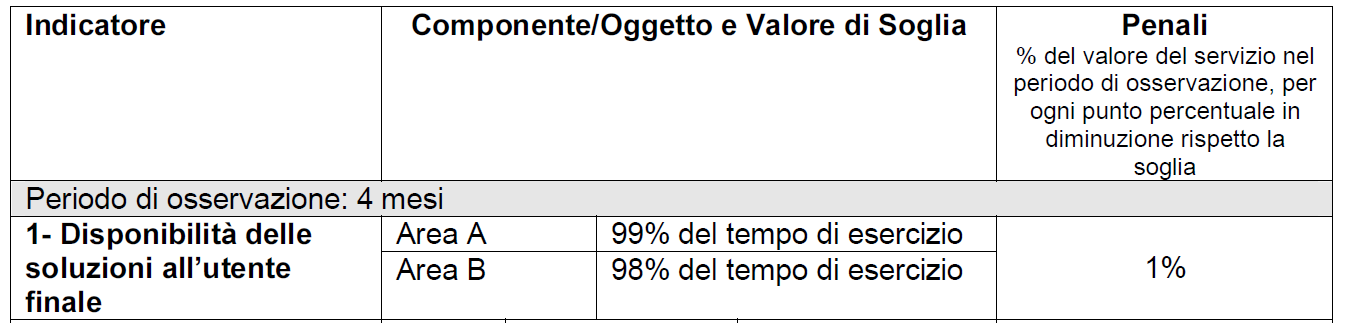
\includegraphics[scale=0.4]{immagini/rollout/sla1}
				\caption{Indicatore globale di servizio "Disponibilità delle soluzioni all'utente finale" (tratto dal Capitolato).}
				\end{figure}
                Considerando il periodo di osservazione di 4 mesi, e considerando una disponibilità pari a 40 ore settimanali in orario lavorativo, il downtime massimo accettato è di circa 6 ore ogni 4 mesi. Questo SLA fa capire che l'accensione dei nuovi sistemi non può permettersi di causare downtime.
                
                
                L'Offerente pianifica di avviare i nuovi sistemi e di eseguire tutte le manutenzioni necessarie in orario non di servizio. In ogni caso date e orari verranno stabilite di comune accordo con il Proponente.
                
		\subsection{Controllo delle performance}
        	Questa sezione descrive tool e tecniche per il monitoraggio e i modi con cui sarà possibile determinare se l'implementazione sta avendo successo.   
            
            
            Controllare periodicamente le performance dell'implementazione è fondamentale per assicurarsi di essere sulla giusta strada e correggere tempestivamente situazioni di errore prima che i problemi diventino troppo gravi. A questo scopo l'Offerente ritiene necessario l'utilizzo di \textbf{metriche} oggettive per la valutazione delle performance che quantifichino il raggiungimento o meno di certi obiettivi.
            
            
            Ad ogni metrica saranno assegnati dei \textbf{range di accettabilità} e di \textbf{ottimalità}, con il seguente significato:
            \begin{itemize}
            	\item Accettabilità: metrica accettabile ma non ottimale. Bisogna continuare ad osservarla con attenzione per rischiare che non degradi nella non accettabilità.
                \item Ottimalità: metrica ottimale, obiettivo pienamente soddisfatto.
            \end{itemize}
            Una metrica che assume un valore all'esterno di questi range non è accettabile e indica un obiettivo non raggiunto: sarà necessario contattare il Capo Progetto al più presto per stabilire delle misure correttive caso per caso. Per situazioni particolarmente gravi sarà necessario contattare il Coordinatore di Progetto (lato Proponente).
            

            \subsubsection{Soddisfazione del Proponente}
            	L'Offerente desidera che il Proponente sia soddisfatto durante tutta la durata dell'implementazione. La soddisfazione verrà misurata tramite dei sondaggi sottoposti mensilmente sia ai clienti che agli utenti, chiedendo loro di valutare in una scala da 1 a 10 la propria soddisfazione.
            	\begin{itemize}
            		\item \textbf{Range:} $[1, 10]$.
                    \item \textbf{Range di accettabilità:} $[6, 7]$.
                    \item \textbf{Range di ottimalità:} $[8, 10]$.
            	\end{itemize}
                Una valutazione insufficiente per più di due volte di seguito da parte dello stesso gruppo di interesse è da ritenersi un segnale d'allarme molto grave e richiederà attenzione immediata da parte del Capo Progetto.
			
            \subsubsection{Tempismo nell'esecuzione dei lavori}
            	L'Offerente desidera che l'esecuzione dei lavori rispetti il più possibile la pianificazione presentata nei Gantt della sezione \ref{sec:attivita} di questo documento. Un ritardo eccessivo potrebbe essere sintomo di problemi gravi non risolti, che rischiano di avere un effetto cumulativo sulle attività successive.
                
                
                Le rilevazioni sul tempismo verranno effettuate ogni due settimane, in coincidenza con la redazione della documentazione di avanzamento progetto da parte dei membri del team dell'Offerente.
                \begin{itemize}
            		\item \textbf{Range:} $[-\infty, +\infty]$ giorni.
                    \item \textbf{Range di accettabilità:} $[8,15]$ giorni.
                    \item \textbf{Range di ottimalità:} $[-\infty, 7]$ giorni.
            	\end{itemize}
                
                
			\subsubsection{Rispetto del budget}
            	L'Offerente desidera che il budget venga rispettato durante tutta l'esecuzione del progetto. Dato che la gestione del budget è legata intrinsecamente ad altre variabili, come qualità, portata e produttività, tenerla sotto controllo è fondamentale per il successo del progetto.

                
                Le rilevazioni sul budget verranno effettuate, come per la metrica precedente, ogni due settimane. Verranno indicate come scostamento percentuale rispetto al budget pianificato per quel periodo.
                \begin{itemize}
            		\item \textbf{Range:} $[-\infty, +\infty] \%$ .
                    \item \textbf{Range di accettabilità:} $[-10, -5), (+5, +10] \%$ .
                    \item \textbf{Range di ottimalità:} $[-5, +5] \%$ .
            	\end{itemize}
			\subsubsection{Rispetto degli SLA}
            	Rispettare gli SLA è fondamentale anche nella fase di implementazione: all'Offerente non è richiesta solamente l'implementazione di un progetto, ma la presa in carico e la fornitura di tutti i servizi IT del Proponente. Concentrarsi esclusivamente sull'implementazione della nuova soluzione e tralasciare la fornitura di servizi di qualità non è accettabile.

                
                Le rilevazioni per questa metrica verranno effettuate mensilmente, anche se il periodo di osservazione per gli SLA identificato nel capitolato risulta essere di 4 mesi. L'Offerente ritiene che misurare con questa frequenza possa dare risultati più tempestivi durante la fase di implementazione.
                \begin{itemize}
            		\item \textbf{Range:} $[0, +\infty]$ SLA violati.
                    \item \textbf{Range di accettabilità:} 0 SLA violati.
                    \item \textbf{Range di ottimalità:} 0 SLA violati.
            	\end{itemize}
                La soglia di accettabilità coincide con quella di ottimalità: questo significa che l'Offerente reputa anche solo la violazione di uno SLA non accettabile.
                

			\subsubsection{Risolvimento incidenti al primo livello}
            	Risolvere gli incidenti al primo livello di contatto (Service Desk) risulta essere fondamentale per non gravare eccessivamente sul personale tecnico, che risulta essere più proficuamente impiegato per l'esecuzione di attività di implementazione e manutenzione. 
                
                
                La rilevazione verrà effettuata su base mensile per tenere sotto controllo le performance del Service Desk.
                
                \begin{itemize}
            		\item\textbf{ Range:} $[0, 100] \% $ incidenti risolti al primo livello.
                    \item \textbf{Range di accettabilità:} $[70, 90] \%$ incidenti risolti al primo livello.
                    \item \textbf{Range di ottimalità:} $[90, 100] \%$ incidenti risolti al primo livello.
            	\end{itemize}
                
		\subsection{Gestione della configurazione}
        	Questa sezione descrive la gestione della configurazione da seguire durante l'implementazione del progetto.
            
            
            Nonostante un'analisi approfondita della gestione della configurazione, scopo del processo di \textbf{Service Asset and Configuration Management}, esuli dagli scopi di questo documento, l'Offerente ritiene utile presentare le metodologie e le convenzioni di massima che intende seguire durante il rollout.
            
            
            Ricordiamo che l'obiettivo del Configuration Management è di fornire un modello logico dell'infrastruttura attraverso l'identificazione, il controllo, la gestione e la verifica di tutte le versioni dei Configuration Items (CI) esistenti. Un CI è un'unità strutturale fondamentale di un sistema di gestione della configurazione. Alcuni esempi di CI sono: documenti, software e componenti hardware. I CI sono memorizzati all'interno di un database, detto CMDB.
            
              Per garantire la possibilità di identificazione univoca, ogni CI sarà identificato da:
              \begin{itemize}
              \item \textbf{ID:} identificativo univoco.
              \item \textbf{Numero di versione:} numero nella forma X.Y.Z che segue le norme del Semantic Versioning (\url{https://semver.org/}). In particolare
              \begin{itemize}
              \item \textbf{X}: numero di versione \textbf{major}, che indica un cambiamento radicale e incompatibile con le versioni precedenti del CI.
              \item \textbf{Y}: numero di versione \textbf{minor}, che indica un'aggiunta di funzionalità al CI compatibile con le versione precedenti.
              \item \textbf{Z}: numero di versione \textbf{patch/emergency}, che indica una risoluzione di problemi del CI compatibile con le versioni precedenti.
              \end{itemize}
              \end{itemize}
              Il numero di versione major 0 dev'essere utilizzato per i CI durante lo sviluppo iniziale. Dopo il go-live, i CI assumono numero di versione 1.0.0.
              
              
              L'Offerente prevede di rilasciare le major release esclusivamente con un approccio \textbf{push}. Questo approccio prevede che l'azione di ricevimento/installazione della release parta centralmente, avviata da parte dell'Offerente. Questa scelta è dovuta al fatto che le major release non sono retrocompatibili e l'Offerente reputa che la gestione di due o più CI con associate due major release diversi potrebbe essere fonte di inefficienze.
              
              
              Per quanto riguarda le minor e le patch/emergency release verranno rilasciate con un approccio \textbf{pull+push}. Questo approccio consiste nel rendere disponibile una release centralmente e permettere agli utenti di applicarla \textit{on-demand} quando lo ritengono necessario. Tuttavia, dato che non c'è garanzia alcuna sul fatto che gli utenti prelevino la release, l'Offerente si occuperà di rilasciare la release in modalità push dopo un certo limite di tempo, di norma una settimana ma variabile in base alla gravità e all'urgenza della release. Così facendo si uniscono i vantaggi della modalità push (rilasciare una release a tutti) a quella pull (dare la possibilità all'utente di scegliere il momento più opportuno per l'installazione).
              
              
		\subsection{Gestione delle sedi}
			La realtà aziendale del Proponente è strutturata su due presidi:
            \begin{enumerate}
            \item La Sede principale di Piazza Cardinal Ferrari.
            \item La Sede di Via Isocrate.
            \end{enumerate}
            L'Offerente si trova chiamato a formulare una strategia per gestire una situazione in cui è necessario effettuare un'implementazione e un rilascio multiplo su due sedi.
            
            
            Data la numerosità e la portata delle attività da eseguire, l'Offerente ritiene migliore adottare una strategia sequenziale piuttosto che parallela, che consiste nello svolgere un'attività prima sulla sede principale e poi sulla sede secondaria. 
            
            
            Seguire questo tipo di strategia porta i seguenti vantaggi:
            \begin{itemize}
            	\item Permette di concentrare maggiormente gli sforzi del team, evitando di disperderli su due realtà diverse.
                \item Permette di eseguire l'attività sulla seconda sede in maniera molto più efficiente, dato che si possono sfruttare gli effetti dell'apprendimento della prima sede, evitando quindi di compiere gli stessi errori due volte.
                \item Garantisce minori rischi dovuti a negligenza, data la maggior concentrazione durante l'esecuzione delle attività.
            \end{itemize}
            Tuttavia, seguire questo tipo di approccio in maniera estrema può portare al completare i lavori nella sede principale prima ancora di averli iniziati nella sede secondaria. L'Offerente vuole evitare questa situazione, dato che porterebbe ad avere sistemi inutilizzati per lungo tempo nella sede principale. La sequenzialità sarà quindi a livello di attività come descritte in sezione 3.2.2: una volta iniziata un'attività, verrà prima completata nella sede principale, e poi ci si concentrerà su quella secondaria. Il \textit{go-live} di sistemi e servizi verrà effettuato solo dopo il completamento dell'attività su entrambe le sedi.
            
              
		\subsection{Criteri di accettazione}
        	Questa sezione identifica i criteri di accettazione per la transizione dalla soluzione esistente alla nuova soluzione.
            
            
            In ognuna delle attività descritte dalla sezione \ref{sec:attivita} sono inclusi i criteri di accettazione per considerare quella specifica attività conclusa. Questa sezione si occupa dell'accettazione di livello più generale, concentrandosi quindi su sistemi e servizi.
            
            
            L'accettazione, anche detta validazione, viene eseguita dal processo di \textbf{Service Validation and Testing}. Il processo è composto dai seguenti sottoprocessi:
            \begin{itemize}
            \item \textbf{Definizione del modello di test:} specifica in dettaglio come la release verrà testata, definendo i \textit{test case} da utilizzare per la validazione.
            \item \textbf{Acquisizione delle componenti della release:} acquisisce le componenti di una release e valuta inizialmente, assicurandosi che solo le componenti che superano dei controlli di qualità stringenti possano essere testate in modo intensivo.
            \item \textbf{Test della release:} testa tutte le componenti e tutti gli strumenti e le tecniche richieste per l'implementazione, la migrazione e il \textit{back out} di una release. Solo le componenti che superano questi test possono entrare nell'ambiente live.
            \item \textbf{Test di accettazione del servizio:} verifica che sussistano tutte le condizioni affinchè il servizio possa essere attivato e ottiene il consenso da parte dell'utente che il servizio rispetta gli SLA concordati.
            \end{itemize}
           
           Seguendo quanto descritto da ITIL, prima del lancio di un servizio o di un sistema esso verrà testato sia internamente da parte dell'Offerente tramite test di unità, integrazione e sistema, sia esternamente, con la presenza del Proponente, in sede di collaudo tramite test di accettazione. 
           
           
           L'Offerente intende seguire l'approccio rappresentato dal seguente modello a V della Verifica e Validazione:
           
            \begin{figure}[H]
				\centering
				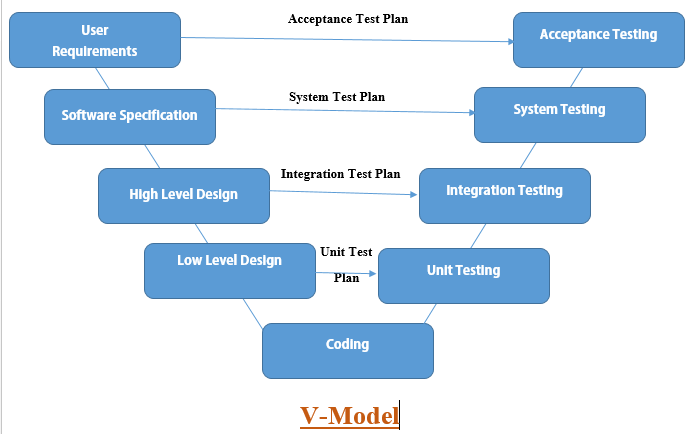
\includegraphics[scale=0.4]{immagini/rollout/v-model}
				\caption{Modello a V della Verifica e Validazione (\url{https://goo.gl/iHMCgV}).}
			\end{figure}
            L'Offerente ritiene fondamentale il successo della validazione esterna con il Proponente. Pertanto, al fine di assicurarsi il successo, verrà posta particolare attenzione all'esecuzione dei test di sistema in modo da certificarne la conformità complessiva.
            
            
            L'Offerente considererà sintomo di gravi problematiche un servizio o sistema che passa i test di sistema interni ma non quelli di accettazione. Qualora dovesse accadere, verranno contattati direttamente il Capo Progetto e il Coordinatore di Progetto per identificare le cause e trovare una soluzione di comune accordo.
            	
            
            
            
            
            
            
            
            
			
            
            
                







             

%\appendix                               
%\input{capitoli/capitolo-A}             % Appendice A

%**************************************************************
% Materiale finale
%**************************************************************
\backmatter
%\printglossaries
%% !TEX encoding = UTF-8
% !TEX TS-program = pdflatex
% !TEX root = ../tesi.tex
% !TEX spellcheck = it-IT

%**************************************************************
% Bibliografia
%**************************************************************

\cleardoublepage
\chapter{Bibliografia}

\nocite{*}
%\printbibliography
%\bibbycategory % equivale a dare un \printbibliography per ogni categoria

\bigskip
\section*{Libri consultati}
Ze-Nian Li, Mark S Drew. Fundamentals of Multimedia, Prentice Hall, 2004:\\
\newline
Peter Symes, Digital Video Compression, Mc Graw Hill, 2003

\vspace{20pt}
\section*{Siti consultati}
\noindent
Paper di ricerca: The H.264 AVC Advanced Video Coding Standard: Overview and Introduction to the Fidelity Range Extensions :\\
URL: \url{http://www.fastvdo.com/spie04/spie04-h264OverviewPaper.pdf}\\
\newline
\noindent
Introducing Daala:\\
URL: \url{https://people.xiph.org/~xiphmont/demo/daala/demo2.shtml
}\\

\end{document}